\documentclass[titlepage,12pt]{report}

\usepackage[utf8]{inputenc}
\usepackage[a4paper, total={6in, 8in},headheight=14pt]{geometry}
\usepackage{newtxtext,newtxmath}
\usepackage[scaled=1]{couriers}
\usepackage[spanish]{babel}
\usepackage{microtype}
\usepackage[bottom]{footmisc}
\usepackage{fancyhdr}
\usepackage{graphicx}
\usepackage{blindtext}
\usepackage{scrextend}
\usepackage{tocloft}
\usepackage{parskip}
\usepackage{multicol}
\usepackage{subcaption}
\usepackage{wrapfig}
\usepackage{multicol}
\usepackage{verbatimbox}
\usepackage[nottoc, notlot, notlof]{tocbibind}
\usepackage{listingsutf8}
\usepackage{url}
\usepackage[square,numbers]{natbib}
\usepackage{adjustbox}
\usepackage[makeroom]{cancel}
\usepackage[hidelinks]{hyperref}
\usepackage[Glenn]{fncychap}
\usepackage{lastpage}
\usepackage{fancyhdr}

\bibliographystyle{unsrtnat}

\pagestyle{fancy}
\fancyhf{}
\fancyhead[R]{\rightmark}
\fancyfoot[C]{\leftmark}
\fancyfoot[R]{\thepage}
\renewcommand{\footrulewidth}{0.6pt}% Line at the footer visible
\addto\captionscatalan{%
  \renewcommand\contentsname{Índice}%
}

\fancypagestyle{plain}{%
  \fancyhf{}%
  \fancyfoot[R]{\thepage}%
  \renewcommand{\headrulewidth}{0pt}% Line at the header invisible
  \renewcommand{\footrulewidth}{0.6pt}% Line at the footer visible
}


\renewcommand{\cftpartleader}{\cftdotfill{\cftdotsep}}%
\renewcommand{\cftsecleader}{\cftdotfill{\cftdotsep}}%
\renewcommand\familydefault{\sfdefault}

\usepackage{tikz}
\usetikzlibrary{shapes.geometric, arrows}

\newcommand{\Lagr}{\mathcal{L}}
\newcommand{\Xagr}{\mathcal{X}}

\setlength{\skip\footins}{1cm}

\makeatletter
% \patchcmd{<cmd>}{<search>}{<replace>}{<success>}{<failure>}
\patchcmd{\@makechapterhead}{\huge}{\large}{}{}% for \chapter
\patchcmd{\@makechapterhead}{\Huge}{\large}{}{}% for \chapter
\patchcmd{\@makeschapterhead}{\Huge}{\large}{}{}% for \chapter*
\makeatother


\begin{document}

\iftrue
\newcommand{\HRule}{\rule{\linewidth}{0.5mm}}

\thispagestyle{empty}

\begin{center}

{\large Universitat Politècnica de Catalunya}

\medskip
{\large Facultat d'Informàtica de Barcelona (FIB)}

\vfill
{\bfseries\Large Bachelor's Degree Project}

\vfill
\centerline{\mbox{
\includegraphics[width=60mm]{media/FIB_UPC.png}}}

\vfill
\vspace{5mm}

{\LARGE Jordi Gil González}

\vspace{15mm}

% Title in English according to the official assignment
{\LARGE\bfseries Analysis of the Path Tracing \\ rendering method on CPU and GPU}

\normalfont \small \sffamily{}

\vfill

Computer Science Department


\vfill

\begin{tabular}{rl}
Bachelor's Degree Project Director: & Chica Calaf, Antoni \\
\noalign{\vspace{2mm}}
Study programme: & Computer Science\\
\noalign{\vspace{2mm}}
Specialization: & Computer Graphics\\
\end{tabular}

\vfill

\large Academic Year 2019/2020

\large \today

\end{center}

\newpage
\thispagestyle{empty}
\section*{Acknowledgement}

First of all I would like to deeply thank Antonio Chica, my project director, for accompanying me in this wonderful and stressful adventure that is the Final Degree Project. When we first talked about doing the FDP together was open to many proposals and it was thanks to their recommendation of Peter Shirley's books and their completion of the Graphics Cards and Accelerators (TGA) course that we were able to define the project.  Secondly, I would like to thank Professor Agustín Fernández, my TGA teacher and member of the "Departament d'Arquitectura de Computadors". Without having any responsibility he moved to get me access to the BOADA cluster. Also, for showing me the way when I was stuck in the CUDA version. To both of you I want to thank you very much for all the patience and enthusiasm you have dedicated to me over the last year.

Finally, I would like to thank all my family and friends for their patience and moral support during the hardest times. I would also like to thank Dawn McRobbie for helping me prepare this project in English.


\selectlanguage{english}
\begin{abstract}
The field of realistic rendering has been investigated for many years. We have different methods capable of creating images with a high degree of realism, such as Ray Tracing, Path Tracing, Photon Mapping or Metropolis Light Transport. Except for Ray Tracing, the rest of the cited methods try to solve the Rendering Equation by approximations (it is impossible to calculate it completely because we would need time and infinite computing power). Thanks to being able to approximate this equation, effects can be achieved naturally, without needing any post-processing, such as motion blur, depth of field, caustics, etc.

The method that we will implement and study is Path Tracing. We will make several versions of this method with which we will explore which architecture (GPU or CPU) gives us a greater advantage in terms of performance for our algorithm. For this, we will have different machines, one with the last generation hardware, one with cheaper hardware and the last machine with hardware thought for a professional environment.

It is very usual that the applications that implement this method are assisted by accelerating structures that allow improving in a very notable way the performance of this one.  For this same reason, we will implement a Bounding Volume Hierarchy, a tree-type structure, to represent our scene and thus increase performance. We will study how to go through it in two different ways, one recursive much more natural in this type of structure and another iterative, to see how it affects the performance of the application on the GPU. It's well known that the GPU is not optimal for recursive functions.

Finally, we'll implement a set of denoising filters. Path tracing produces very noisy images when using a few samples per pixel, so the use of denoising filters is very common. This will also help us find a balance between the number of samples per pixel and the need for post-filtering of the output image.
\end{abstract}

\selectlanguage{catalan}
\begin{abstract}
Fa molts anys que es realitza recerca al camp de la renderització realista. Tenim diversos mètodes capaços d’aconseguir imatges amb un gran grau de realisme, com pot ser Ray Tracing, Path Tracing, Photon Mapping o Metropolis Light Transport. A excepció del Ray Tracing, la resta de mètodes tracten de resoldre l'Equació de Renderitzat mitjançant aproximacions (és impossible calcular-la íntegrament, ja que necessitaríem temps i potència de càlcul infinita). Gràcies a poder aproximar aquesta equació es poden aconseguir efectes de forma natural, sense necessitat d’un postprocessat, com motion blur, depth of field, càustiques, etc.

El mètode que implementarem i estudiarem és el Path Tracing. Realitzarem diverses versions d’aquest mètode amb les quals podrem explorar quina arquitectura (GPU o CPU) ens ofereix una major avantatge pel que fa al rendiment per al nostre algoritme. Per això comptarem amb diverses màquines, una amb un hardware d’última generació, una amb un hardware més econòmic i una última màquina pensada per un entorn professional.

És molt usual que les aplicacions que implementen aquest mètode s’utilitzen d’estructures de dades que permeten millorar de forma molt notable el rendiment d’aquesta. Per aquesta raó, implementarem una Bounding Volume Hierarchy, un estructura de tipus arbre, per a la representació de l'escena i així augmentar el rendiment. Estudiarem com recorre-la de dues formes diferents, una recursiva molt més natural en aquest tipus d'estructures i un altre iterativa, per veure com afecta al rendiment de l’aplicació en la GPU. És ben sabut que les funcions recursives no són gens òptimes a la GPU.

Per últim, implementarem un seguit de filtres d’eliminació de soroll. El mètode de Path Tracing produeix imatges molt sorolloses si s’utilitzen poques mostres per píxel, per això l’ús de filtres d’eliminació de soroll és molt comú. Això ens permetrà trobar un equilibri entre el nombre de mostres per píxel i la necessitat d’un postfiltratge de la imatge resultant.

\end{abstract}

\selectlanguage{spanish}
\begin{abstract}
Desde hace muchos años se lleva investigando el campo de renderización realista. Tenemos diferentes métodos capaces de conseguir imágenes con un gran grado de realismo, como por ejemplo Ray Tracing, Path Tracing, Photon Mapping o Metropolis Light Transport. A excepción del Ray Tracing, el resto de métodos mencionados tratan de resolver la Ecuación de Renderizado mediante aproximaciones (es imposible calcularla íntegramente, debido a que necesitaríamos tiempo y potencia de cálculo infinita). Gracias a poder aproximar esta ecuación se pueden conseguir efectos de forma natural, sin necesidad de post-procesado, como motion blur, depth of field, cáusticas, etc.

El método que implementaremos y estudiaremos es el Path Tracing. Realizaremos varias versiones de este método con las que exploraremos que arquitectura (GPU o CPU) nos proporciona una mayor ventaja en cuanto a rendimiento para nuestro algoritmo. Para ello contaremos con diferentes maquinas, una con un hardware de última generación, una con un hardware más económico y la última maquina con hardware pensado para un entorno profesional.

Es muy usual que las aplicaciones que implementan este método se utilizan de estructuras aceleradoras que permiten mejorar de forma muy notable el rendimiento de esta. Por esto mismo, implementaremos una Bounding Volume Hierarchy, una estructura de tipo árbol, para representar nuestra escena y aumentar así el rendimiento. Estudiaremos como recorrerla de dos formas diferentes, una recursiva mucho más natural en este tipo de estructuras y otra iterativa, para ver como afecta al rendimiento de la aplicación en la GPU. Es bien sabido que en la GPU las funciones recursivas no son óptimas.

Por último, implementaremos una serie de filtros de eliminación de ruido. El método de Path Tracing produce imágenes muy ruidosas si se utilizan pocas muestras por píxel, por lo que el uso de filtros de eliminación de ruido es muy común. Esto también nos ayudará a encontrar un equilibrio entre el número de muestras por píxel y la necesidad de un post-filtrado de la imagen resultante.

\end{abstract}
\selectlanguage{english}
\tableofcontents*
\fi
\newpage

\chapter{Contextualization and Scope of the project}

\section{Introduction} \label{introduction}

Nowadays, the images generated by computers are very present in both a work and entertainment environment. The creation of realistic images through computer programs has become a necessity. Industries like the film or video games need algorithms capable of representing the real world in a virtual one and, whenever possible, in the shortest possible time.

The study about methods that allow rendering realistic images is not new. Between the early and mid-70s, the first papers about the simulation of light and colours over the surface of three-dimensional models began to be published. To understand how these methods work, we have to keep in mind the common representation of 3D models.

To represent a 3D model it uses a ''polygon mesh'', commonly known as a triangle mesh because, the triangle, is the most used polygon. This mesh consists of a set of vertices connected through edges and creating faces.  For all face, we can define an orthogonal normal vector. In Figure \ref{dolphin} we can see an example of a 3D model represented by a triangle mesh.

\begin{figure}[H]
	\centering
	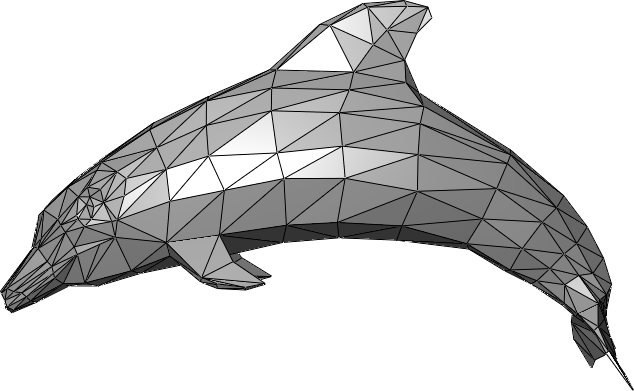
\includegraphics[scale=0.15]{media/Dolphin_triangle_mesh.png}
	\caption{Triangle mesh example. Source: Wikipedia}
	\label{dolphin}
\end{figure}

Returning to lighting calculation methods, the simplest is the \textit{Flat Shading}. This method only uses one of all the vertices that make it up and her normal to determine the colour of each face of our mesh. In a mesh represented by triangles, it's commonly using the centroid of the triangle. The colour it's interpolated for each vertex. Every face is computed independently, and this produces a visual difference result between continuous faces. In Figure \ref{flat:shading}, we can see an object rendered using this method. We might think that adding more vertices improve the results, but is not the solution because when more vertices have our meshes, more memory is required and the problem would not be solved. Also, if we zoomed in at the 3D model, we would see the same effect (known as Mach bands) \citep[pp.~5245--5250]{Lotto1999}.

\begin{figure}[H]
	\centering
	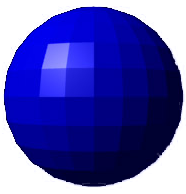
\includegraphics[scale=0.5]{media/Flat-shading-sample.png}
	\caption{Example of \textit{Flat Shading}. Source: Wikipedia}
	\label{flat:shading}
\end{figure}

In the smooth shading methods, the colour change between pixels instead of faces. The result is a smooth transition of colour between adjacent faces. In 1971 Henri Gouraud presents us in his paper \textit{Continuous Shading of Curved Surfaces} \citep[pp.~623--629]{Henri1971} the Gouraud Shading. With this method, we can add more continuity to the shading, unlike the Flat Shading. The great improvement concerning the method presented above is that it does not require a high-density mesh to simulate greater continuity. For each pixel it's intensity is determined by interpolation of the intensities defined at the vertex of each polygon.

\begin{itemize}
	\item For each vertex, a normal is defined as the average of the normals of the polygons to which said vertex belongs.
	\item Through the using of some lighting model,  e.g. the Phong reflection model, the intensity of each vertex is computed using the normal taken in the previous point.
	\item For each pixel, the intensity it's interpolated on every vertex to get his intensity.
\end{itemize} 

As we can see in Figure \ref{Gouraud:shading}, the results are notably higher, however, it does not represent the specular highlights. These would be a problem if they appear in the centre of a face.

\begin{figure}[ht]
	\centering
	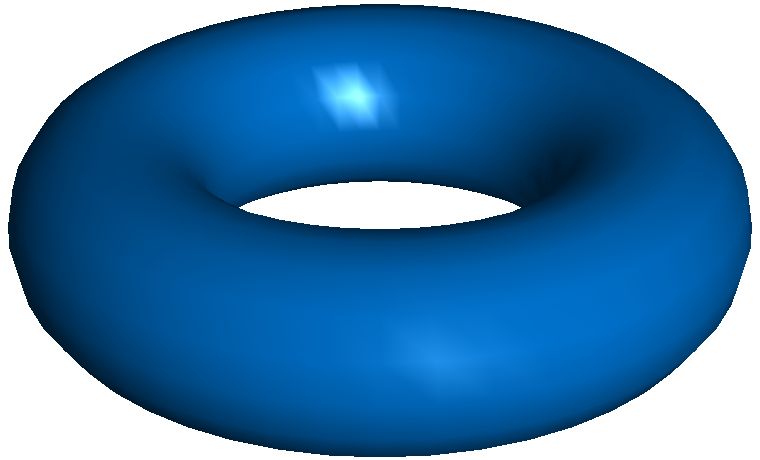
\includegraphics[scale=0.25]{media/Gouraudshading00.png}
	\caption{Ejemplo de \textit{Gouraud Shading}. Source: Wikipedia}
	\label{Gouraud:shading}
\end{figure}

Later, in 1975, Bui Tuong Phong in his PhD thesis \citep[pp.~311--317]{Phong1975} introduces to us the Phong Shading. In the method presented by Phong, instead of calculating the intensity at the vertex, first of all, the normal is defined, interpolated and normalized for each pixel and then using some lighting model the final intensity is determined. Computationally, this method is expensive regarding the others presented, because the calculation is made at fragment (pixel) level.

Phong mention in his paper published by the ACM \citep[p.~311]{Phong1975} that his goal was not to simulate the reality, but rather to add more realism:
\vspace{5mm}

\begin{mdframed}[hidealllines=true,backgroundcolor=gray!20] ''\textit{In trying to improve the quality of the synthetic images, we do not expect to be able to display the object exactly as it would appear in reality, with texture, overcast shadows, etc. We hope only to display an image that approximates the real object closely enough to provide a certain degree of realism.}'' 
\end{mdframed}

Even though these methods represented, as far as realism is concerned, an advance, they do not pretend to simulate reality. Furthermore, these only take into account ambient, diffuse and specular light. They do not take into account the indirect lighting of the scene, an important factor in creating images that produce realistic effects such as reflections.

It was not until the 80s that the first methods capable of rendering realistic images appeared. At the sixth annual conference on \textit{Computer graphics and interactive techniques (SIGGRAPH)}, Turner White presents the Ray Tracing method \citep[pp.~343--349]{Whitted1980}. This method is based on the Ray Casting algorithm, presented by \citep[pp.~37--45]{Appel1968}, which consists of tracing rays from the observer to all pixels, on for each one, to determine the closest object. Also, once the ray hits on a surface, based on the properties of the materials defined and the light properties, the colour is computed. Also, using texture maps we can simulate shadows.

In 1986, David Immel et al. and James T. Kajiya, researchers from Cornell University and California Institute of Technology (Caltech) respectively, at the thirteenth annual conference on \textit{Computer graphics and interactive techniques (SIGGRAPH)} they introduced the \textit{Rendering Equation} \citep[pp.~143--150, pp.~133--142]{Kajiya1986, Immel1986}. This integral equation tries to summarize in one formula how the light interacts with a surface when a ray of light hits her using a bidirectional reflectance distribution function (BRDF). This formula takes into account the number of photons from the source, the incident angle, etcetera.

Exist other methods that can generate realistic images by approximating the RE: Bidirectional Path Tracing, presented by \citep[pp.~145--153]{Lafortune1993}; Photon Mapping, formulated by \citep[pp. ~21--30]{Jensen1996}; Metropolis light Transport, introduced by \citep[pp. ~65--76]{Veach1997}.

\newpage

\section{Contextualization}

\subsection{Context}

During the degree studies, there are some subjects dedicated to computer graphics. In these subjects, we are introduced to realistic rendering methods, but beyond the theoretical introduction to these, they are never put in practice. From here comes the idea of realizing the present project, to be able to go deeper into the subject of realistic rendering and thus create an application based on what has been learned during the studies. Other aspects of computer science seen will also put into practice, such as the creation of parallel applications on both CPUs and GPUs.

As we have pointed out in the last section, rendering true-to-life images is an area of great enthusiasms in computer graphics. One of the principal goals is to be able to render images that are indistinguishable from photos. Following this idea, being able to simulate the behaviour of light in a virtual environment is an important task. It's essential to keep in mind the global illumination of our scene to achieve that realism. The global illumination is compounded by \begin{enumerate*}[label=\roman*)] \item direct illumination \label{item:dl} and \item indirect (global) illumination \label{item:il} \end{enumerate*}. In Figure \ref{globalil}, we can observe a visual description of both types of lighting.

\begin{figure}[!ht]
	\centering
	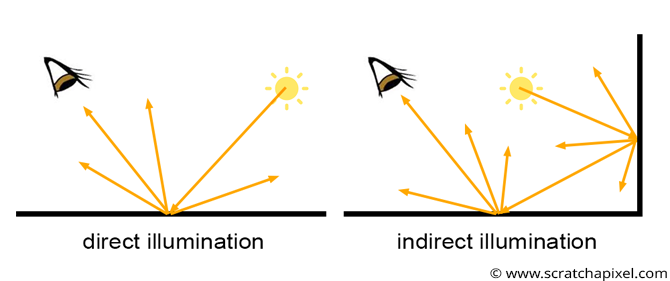
\includegraphics[scale=0.45]{media/shad2-globalillum3.png}
	\caption{Example of \textit{Direct illumination and Indirect illumination}. Source: ScratchPixel}
	\label{globalil}
\end{figure}

\ref{item:dl} Direct illumination is that which strikes a point from the light source.\\
\ref{item:il} Indirect illumination is that which hits one point from the light bouncing off other points in the scene.

Retrieving what was said in the introduction, the first method capable to render realistic images was the Ray Tracing, based on Ray Casting algorithm, a technique that consists in trace rays from the eye or camera to all the pixels of an image. The great innovation concerning the algorithm presented by Appel is the recursivity. The Ray Tracing algorithm emits a ray from the virtual camera across the scene to a light source. When a ray hits some surface can produce three new types of rays: \begin{enumerate*}[label=\roman*)] \item reflection ray\label{ray:reflected}, \item refraction ray and \item shadow ray\end{enumerate*}. From this point, a new ray is projected until hits one of the light sources in the scene. When tracing new rays, we can obtain effects like reflections, shadows, caustics, etcetera. If the ray hits a transparent material like glass, then the ray is projected through this to simulate the refraction rays. The principal disadvantage is the dependency on the number of polygons in the scene. The more polygons the scene will have, the more inefficient will be the algorithm.

The results obtained are not necessarily photo-realistic despite offering a high degree of realism by being able to accurately treat optical effects such as refraction or reflection. It's mandatory to do some post-processing to be able to simulate effects such as soft shadows or caustics. To render photo-realistic images is mandatory approximating the RE. The Path Tracing algorithm, presented by \citep[pp. ~143--150]{Kajiya1986}, is a good precedent.

The Path Tracing algorithm came up as an improvement of the Ray Tracing with the purpose to give a solution of the rendering equation by the Monte Carlo integration. It is for this reason that the algorithm is inherently able to simulate effects such as motion blur, ambient occlusion and global illumination without any post-processing. Unlike Ray Tracing, in the Path Tracing when a ray is emitted by the virtual camera, this is traced through the scene bouncing in the objects until reaching one light source, sky or run out a limit. The significant difference between the algorithm presented by White is that in the algorithm introduced by Kajiya, for each pixel we keep in mind not only one ray but dozens, hundreds or even thousands. The random sampling is an important aspect, this implies that when a  ray hits a surface, it generates a new ray in a random direction. Once a ray reaches a limit or it is absorbed by a light source, the colour is calculated according to the material properties of the objects it has bounced off. This colour is added to compute the average between all rays emitted for each pixel. This random sampling produces a noisy result. The more sampling we use, the smoother it becomes the output image.

\begin{figure}[!ht]
	\centering
	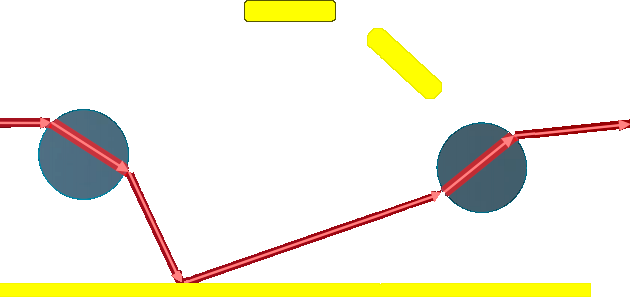
\includegraphics[scale=0.45]{media/lightPathRT.png}
	\caption{Ray Tracing}
	\label{RT_traced}
\end{figure}

\begin{figure}[!ht]
	\centering
	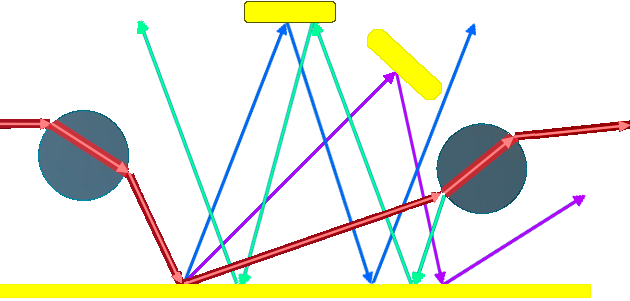
\includegraphics[scale=0.45]{media/lightPathPT.png}
	\caption{Path Tracing}
	\label{PT_traced}
\end{figure}

In Figure \ref{RT_traced} it can be observed what is mentioned in the previous paragraph. In the Ray Tracing, the colour calculation in one pixel depends only on the primary ray and his bounces until reach a light source. However, in Figure 5 it can be observed that for each bounced, multiple rays are traced. This occurs because when a ray hits a diffuse surface, the photons are scattered in all directions. 

The number of polygons in a scene is less important for Path Tracing. The scene complexity does not affect proportionally to the algorithm's performance. How we mentioned above, in the first method only one ray is traced for each polygon. However, in Kajiya's method, the ray is traced per pixel. We can exploit the concurrency provided by CPUs and GPUs because each pixel is independent of each other.

\begin{figure}[H]
	\centering
	\begin{subfigure}{.3\textwidth}
		\centering
		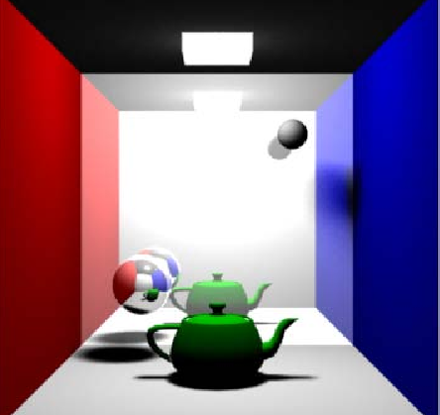
\includegraphics[width=.8\textwidth]{media/RayTracing.png}
		\caption{\textit{Ray Tracing}.}
		\label{RT}
	\end{subfigure}
	\begin{subfigure}{.3\textwidth}
		\centering
		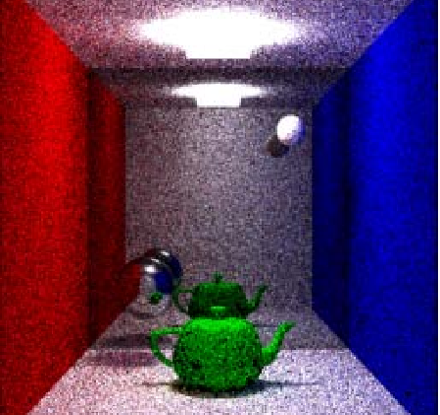
\includegraphics[width=.8\textwidth]{media/PathTracing.png}
		\caption{\textit{Path Tracing} with noise.}
		\label{PTN}
	\end{subfigure}
	\begin{subfigure}{.3\textwidth}
		\centering
		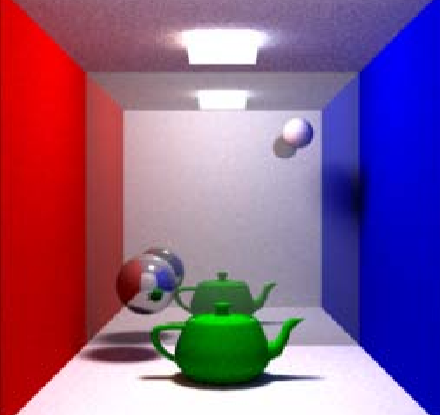
\includegraphics[width=.8\textwidth]{media/PathTracingMD.png}	
		\caption{\textit{Path Tracing} without noise.}
		\label{PT}
	\end{subfigure}
	\caption{Comparison \textit{Ray Tracing vs. Path Tracing}. Source: \citep[pp.~23--29]{Cassagnabere2004}}
\end{figure}

We can observe how the Path Tracing, in Figure \ref{RT}, produces soft shadows compared to Ray Tracing, Figure \ref{PT}. Also, we can see the noisy effect produced by the random sampling of Path Tracing if the number of samples is poor.

In the present project, we are going to create an application that implements the Path Tracing method attempting to generate images that looks realistic. This application it's going to compute each pixel of an image given some scene. There will be three versions. The first one is the sequential version where one pixel is computed at once, and it's the base for all other versions. The other two versions are the CPU and GPU parallel versions. The reason to develop all of these versions is to be able to do a performance analysis of our algorithm both in GPU and CPU and decide which architecture is bringing more performance.

The implementation proposed by Peter Shirley in his books about Ray Tracing  \citep{ShirleyRTA, ShirleyRTB, ShirleyRTC} is going to be the base to develop our Path Tracer. The main intention is to develop three applications (sequential in CPU, parallel in CPU and GPU) to analyse how is the performance in both architectures CPU and GPU.

We will not only focus on the rendering section, although this is the central thread of this project, but we will also study which acceleration techniques are commonly used to try to improve our algorithm as much as possible. That is why we will also study which is the best way to represent internally the scene we want to render following the idea presented by \citep{Karras2012} in his paper.

The way we represent our scene will have a great impact on how we compute the colour of the final image. As we have mentioned above, the basis of the method is to trace rays through the scene to compute the colour of each pixel. If our representation of the scene consists of storing all the objects in a data structure such as a list or vector ordered by creation when calculating a point of the image in the worst case we will be going through the whole set of polygons of the scene to determine the final colour. Trying to render a scene that, very possibly, is composed of thousands of polygons can translate into hours and hours of processing. That's why we'll make use of an accelerating data structure that allows us to represent the scene in a more clever way, so that when determining if a ray hits or not a polygon is determined in the fastest way possible.

\subsection{Stakeholders}

In this section, we are going to describe the different actors involved in a project.

\subsubsection{Developer}

This actor is in charge of planning, information search, documentation, development of the required software, solution of possible obstacles and difficulties that may arise throughout the development, and performance and analysis of the experiments. He needs to work in coordination with the director, and co-director if it exists. Also, is the last person in charge of fulfilling the established terms.

\subsubsection{Project director}

This actor is in charge of leading the developer in case of difficulties, as well as advising on possible solutions.

\subsubsection{Benefited users}

Despite this project has not the intention to create a product on its own, it doesn't mean that there are not benefited users. Investigating the different ways of optimization using parallel architectures can be useful for many researchers or developers.

\section{Justification}

As we have already pointed in the above section, we will start from the Peter Sherly books and Tero Karras paper about Bounding Volume Hierarchies. In this project, we expect to study how we can exploit at maximum the different architectures that we have in our computers (CPU and GPU) and decide how's more efficient. We cannot compare our application with an existing one. Because the professional applications that implement the Path Tracing algorithm are made by experts with plenty of experience and knowledge that will allow increasing the performance significantly, and the author of this project does not have. Moreover, in the field of realism, it's hard to compare because a professional application includes plenty of features such as subsurface scattering or tessellation and for this project, it's impossible to reach an application with similar characteristics. First, the lack of knowledge and experience in the field of realistic off-line rendering.
Finally, the time. Usually, a project with this scope involves plenty of specialists and need months or years to realize. A professional example of Path Tracer is RenderMan, developed by Pixar Animation Studios \citep{Christensen2018}.

For this reason, in this project, we will develop three versions of the same algorithm: \begin{enumerate*}[label=\roman*)] \item sequential version, \item parallel version in CPU and \item parallel version in GPU \end{enumerate*}. Therefore, we will analyse the versions with each other and decide the best architecture and version for our implementation.

Currently, there are plenty of libraries oriented to GPU programming. Libraries such as \texttt{OpenCL} and \texttt{OpenACC} provides us with portability between graphics cards from different manufacturers like \texttt{AMD} and \texttt{NVIDIA}. For this project, we decided to choose the CUDA environment developed by \texttt{NVIDIA}. \texttt{CUDA} is a parallel computing platform and API created for its graphics card and accelerators. The reason we chose this API is that being proprietary software it is more optimized for \texttt{NVIDIA} graphics cards, as indicated by \citep{Karimi2010} and \citep[pp.~216--215]{Fang2011} in their respective papers.

It is possible that citing the \texttt{NVIDIA} graphics cards and accelerators and, keeping in mind the project's focus on rendering realistic graphics, to the lector of this Final Degree Project comes to mind the new brand of RTX cards designed by \texttt{NVIDIA}. In the beginning, the idea was to orient the project to use RTX graphics cards because they have been designed specifically for the use of Ray Tracing in real-time. But, this idea was immediately rejected because of the high price of these. The price range varies between €350 to €2000 or €6000 (for HPC). Finally, even the author of this project bought an RTX 2080 Super it was decided not to focus the project only in the new RTX technology. Exploring all the new features that these include such as RT Cores, Tensor Cores and Mesh Shaders would have meant starting the job all over again and losing a huge amount of time spent. Because it, would have been necessary to learn all the necessary knowledge to develop the project. That does not imply that the graphics card should not be used. As a high-end graphics card, the number of cores it has compared to the GTX1050 (mid-range) will allow us to analyse how much better it is and whether it is worthwhile, in terms of cost/power ratio, to use it in applications of this type.

As we mentioned at the beginning of this section,  \texttt{CUDA} is an API very optimized for \texttt{NVIDIA} hardware. This gives us an advantage because all the environments that we will use in this project have NVIDIA technology.

\begin{enumerate}
	\item Laptop - Lenovo Legion Y520 with an Nvidia GTX1050 Mobile - 4GB.
	\item Personal Computer - Nvidia RTX 2080 Super - 8Gb.
	\item Teaching cluster BOADA - 4 GPUs Nvidia Tesla K40c.
\end{enumerate}

The use of graphics cards in different environments will allow us to analyse how our application responds in each of them and thus study how performance is when we use several cards designed for a research/professional environment, as opposed to two others designed for more ordinary use. We will also be able to see how the performance is in a mid-range graphics card (Nvidia GTX1050 Mobile) and a high range one (Nvidia RTX 2080 Super) and make a comparison between them.

\section{Project Scope}

To solve the problem presented in our project, we need an application that can render realistic-look images. As we notice a few sections back, \citep{ShirleyRTA, ShirleyRTB, ShirleyRTC} presents the principles to create a Ray Tracing. We are going to use this to develop our main parallel application on CPU and GPU.

Furthermore, as we said in the context section, the use of acceleration structures is a significant factor in this type of applications, and they have been studying for many years by the science community, e.g. \citep{Rubin1980}. In this project, we will use the \textit{
Bounding Volume Hierarchy} (BVH), a tree structure (binary or n-ary) where each leaf represents the bounding box of each primitive; and each internal node the bounding box of his children.

There are many ways to build a BVH, but we decided to develop the version proposed by \citep{Karras2012, Karras2013}. We can build each internal node independently using the concurrence provided by the GPU and CPU.

\subsection{Objectives}

\subsubsection{Main objectives}

There are several main objectives that we propose in the project. The first one is to develop three applications (sequential, CPU parallel and GPU parallel) in which given a scene will render it using the \textit{Path Tracing} method, and we will analyse the performance given by all versions developed to determine who have a better performance.

A second main objective is studying and implementing what are the best practices about memory management in a parallel application. We identified it as one of the main goals because inadequate management of it can be a serious obstacle in the development of the project.

\subsubsection{Secondary objectives}

The secondary objectives, but no less important, are the following:

\begin{enumerate}
	\item Efficiently implement the methods presented by Peter Shirley and Tero Karras.
	\item Find information about optimization techniques in the calculation of ray-object intersection.
	\item Efficiently implement ray-object intersection calculations.
	\item \label{3D} Extend the application to render 3D models.
	\item \label{GLUT} Develop an interactive application.
\end{enumerate}

The secondary objectives \ref{3D} and \ref{GLUT} will be realized according to the time remaining for the completion of the project.

\subsection{Obstacles and risk}

Although the main topics dealt with in this project have been thoroughly studied, this does not mean that the development of this project is an easy task since there are many problems or obstacles that we may face.

\subsubsection{Main program}

As we said in the previous section, the memory management it's very important. An improper manage of this may cause errors that don't allow the correct functioning of the application.

\subsubsection{Algorithm}

The algorithm that we will use computes the colour from the ray-object intersection. In the process of generating an image, these intersections are made billions of time, so an improper/inefficient implementation of the calculations can affect the performance of our application negatively.

\section{Methodology and rigour}

In this section, we're going to look at the set of tools that we're going to use during the development of the project. To be able to carry out a good development of the project, we will organize ourselves in the following form: \begin{enumerate*}[label=\roman*)] \item Meetings every 15 days with the director to discuss the state of the project, results obtained, objectives fulfilled and determine the next steps. \item Meetings weeklies in the final phase. \end{enumerate*}

\subsection{Methodology}

The work methodology that we will follow in this project is agile. This methodology breaks development in small task to minimize the amount of planning. Each iteration, or sprint, has a set of assignments. In our project, each iteration of the development cycle will correspond with a meeting with the director until the next meeting. All meeting needs specifying the objectives to achieve to the next sprint. In Figure \ref{agile}, we can see a scheme of how agile methodology works.

\begin{figure}[ht]
	\centering
	
\includegraphics[scale=0.25]{media/agile.png}
	\caption{Agile methodology scheme. Source: OpenWebinars}
	\label{agile}
\end{figure}

\section{Development tools}

The programming language that we will use to develop our project is English using the \texttt{OpenMP} and \texttt{CUDA} libraries.

\texttt{OpenMP} is an API design to add concurrence to programs written in \texttt{C}, \texttt{C++} and \texttt{Fortran}. The main advantage against others with similar characteristics is the portability between different Operating Systems.

\texttt{CUDA} is a parallel computing platform and \texttt{API} developed by \texttt{NVIDIA} that allows us to access to a set of instructions and compute elements inside the graphics cards and accelerators to create parallel applications.

\section{Monitoring tools}

To monitor the development of this project, we will use git to track all versions and consult them if necessary.

\chapter{Project Management}

\section{Planning}

This chapter deals with project planning and describes the tasks performed, through an action plan, to meet the deadlines relating to the delivery of the project. We will also present the resources used and analyse the possible obstacles that could modify the planning.

The project began in early July 2019 with a deadline on 13 January 2020. Finally, the delivery was postponed to April of the same year.

\section{Task description and resources used}

\subsection{Task description}

\subsubsection{Study of concepts}

Before starting the project, it was necessary to become familiar with the basic concepts relative to our project. There were a couple of meetings with the project director, during the previous semester, to define the topic of the project. Also, the author of this project enrolled in the subject of Graphics Cards and Accelerators (TGA for her acronym in Catalan) to introduce himself in the parallel computing platform \texttt{CUDA}. Since this task is carried out outside the project plus the difficulty of determining an estimate in hours, it will not be taken into account in the planning.

\subsubsection{System configuration}

Before starting the development, we need to configure the necessary tools and guarantee her correct functioning.

To be able to develop our project it is mandatory to have installed \texttt{CUDA} in our systems. The \texttt{OpenMP} libraries are installed by default on Linux systems, so no installation is required, but it is necessary to check that they work properly. To finish, we will make use of \textit{TexMaker}, a word processor that allows to us compile \LaTeX code to create our documentation.

The laptop and personal computer need setting up. The BOADA Cluster no needs a previous configuration because it has already been configured by the DAC (Departament d'Arquitectura de Computadors).

\subsubsection{Project Planning}

This task corresponds to the content covered by the GEP course. We can split them into three sub-tasks:

\begin{enumerate}
		\item Context and scope of the project.
		\item Time planning.
		\item Budget and sustainability.
\end{enumerate}

\subsubsection{Development}

Development task is the most important of all project. Includes the development of all three applications, results and documentation. We will split this phase in cycles of 14 days each one. Each cycle will have four subtasks:

\begin{itemize}

	\item \textbf{Sequential version development:} This version is the basis for the parallel applications.
	
	\item \textbf{CPU parallel version development:} Once the sequential version has been developed, we will translate them to CPU parallel version using the \texttt{OpenMP} library. 
	
	\item \textbf{GPU parallel version development:} Once the sequential version has been developed, we will translate them to CPU parallel version using the \texttt{CUDA} library. 

	\item \textbf{Results:} Using the three applications, we will render the defined scenes and will study the performance in each one of them.

\end{itemize}

The dependencies between the different tasks are easy to explain. Until we have not the sequential version, we can't start programming the parallel versions of this one. Nor can we start a new cycle without having finished the previous one.

\subsubsection{Final stage}

In this stage, we will structure all the documentation of the previous stages and prepare the defence.

\subsection{Summary table and estimation}

\begin{table}[H]
	\centering
	\begin{tabular}{|m{5cm}||m{5cm}|}
		\hline
		Task & Time spent (horas) \\ \hline \hline
		System configuration & 10 \\ \hline
		Project planning & 133 \\ \hline
		Development & 546 \\ \hline
		Final Stage & 65 \\ \hline \hline
		Total & 754 \\ \hline
	\end{tabular}
	\caption{Hours Summary}
\end{table}

With an estimation of 35 hours per week (3 hours from Monday to Thursday and 10 hours Saturdays and Sundays), and keeping in mind a total of 30 weeks of work, we have $35h*30 = 1050$ hours estimated.

\subsection{Resources used}

\subsubsection{Software}

\begin{itemize}
	\item Linux, used in all task.
	\item \LaTeX , for documentation.
	\item \texttt{C++},\texttt{OpenMP} and \texttt{CUDA}, for the development of the applications.
	\item \texttt{git}, used for version control and code sharing between different environments.
\end{itemize}

\subsubsection{Hardware}

\begin{itemize}
	\item Desktop PC with the following features: i7 7700 3.6 GHz, NVIDIA GeForce RTX 2080 SUPER, 24GB RAM, 250 SSD, 1TB SSD, 1TB HDD
	\item Laptop with the following features: i7 7700HQ 2.8GHz, NVIDIA GeForce 1050 Mobile, 8GB RAM, 500GB SSD
	\item Teaching cluster with the following features: Intel Xeon E5-2620 v2 2.10GHz x2, NVIDIA Tesla K40c x4, 64GB RAM, 1TB x2
\end{itemize}

\section{Risk management: Alternative plans and obstacles}

During the development may occur some obstacles or deviations that can alter the initial planning. Thanks to the agile methodology, it is easy to manage the mishaps that may arise. The main objectives were clearly and concisely defined, and this has allowed us to know in all moments which goals have been reached and have not.

The hours planned for the different task are not static. We may need more hours, or we may even have hours left over that we can spend on other tasks.

Besides, in the case of not being able to provide different shapes to represent our 3D models such as spheres or triangles, we will only use triangles because of the versatility that these give us.

\section{Knowledge Integration}

Principally, the knowledge integrated into the project corresponds to the knowledge acquired in the Computer Science speciality, as well as some obligatory subjects of the degree and optional ones. The familiarity about realistic rendering and application of geometric transforms on 3D objects, discussed in the subject of graphics, has been required. Also, the topics studied in subjects such as Parallelism and TGA, have been very important to develop our parallel applications.

Having knowledge in programming in languages like \texttt{C} or \texttt{C++} has been important for the proper development of the project.

\section{Identification of laws and regulations}

As we said in the first delivery, the main objective of the project is to allow the author to enter the field of computer rendering, in particular realistic rendering. For this reason, there are no laws or regulations that can be applied because it is not intended to make a commercial product. Furthermore, all the materials and tools used during the project are for free use or self-created.

\chapter{Budget and sustainability}

In this chapter, we will present two significant topics, budget and sustainability. We will provide a detailed description of the costs of the project, of both material and human resources, and an analysis of how the different obstacles that may occur during the development could change our budget. We will also assess the sustainability of the project.

\section{Budget}

In this section we will make an estimate of the budget to develop the project. We can divide the budget in two big sections: \begin{enumerate*}[label=\roman*)] \item Direct costs and \item Indirect costs \end{enumerate*}.

\subsection{Direct costs}

We divide the direct cost into the three types of resources that we have in the project: \begin{enumerate*}[label=\roman*)] \item software \item hardware and \item human \end{enumerate*}.

For the calculation of the amortization, we will take into consideration that the project has a duration of approximately eight months.

\subsubsection{Software resources}

All the software that we will use in our project is open source. The table \ref{soft} shows the cost of all software used.

\begin{table}[H]
	\centering
	\begin{tabular}{|c|c|c|c|}
		\hline
		\textbf{Product} & \textbf{Price} & \textbf{Lifetime} & \textbf{Amortization} \\ \hline \hline
		Ubuntu 18.04 	& 0,00€ & - & 0,00€ \\ \hline
		\LaTeX\ 		& 0,00€ & - & 0,00€ \\ \hline
		CUDA 			& 0,00€ & - & 0,00€ \\ \hline
		OpenMP 			& 0,00€ & - & 0,00€ \\ \hline
		C++ 			& 0,00€ & - & 0,00€ \\ \hline	\hline
		Total 			& 0,00€ & - & 0,00€ \\ \hline
	\end{tabular}
	\caption{Software resources cost}
	\label{soft}
\end{table}

\subsubsection{Hardware resources}

The table \ref{hard} shows the cost of all hardware used to develop the project. The amortization takes into account an approximate duration of eight months of the project as we have specified at the beginning of this section. Approximately one year have 365 days and the lifetime of the machines used is 5 years, then this gives us a total of 1825 days of life for the computers. The project lasts from September to April therefore the total duration is 243 days.

\begin{table}[H]
	\centering
	\resizebox{\textwidth}{!}{\begin{tabular}{|c|c|c|c|c|}
		\hline
		\textbf{Product} 	& \textbf{Price} & \textbf{Lifetime (in years)} & \textbf{Amortization/day} & \textbf{Amortization} \\ \hline \hline
		Desktop PC 		& 2210,09€ & 5 & 1,21€/día & 294,03€\\ \hline
		Lenovo Legion Y520 	&  900,00€ & 5 & 0,49€/día & 119,07€ \\ \hline
		BOADA 				& 3500.00€ & 5 & 1,92€/día & 466,56€ \\ \hline \hline	
		Total 				& 6610.09€ & - & -         & 879,65€ \\ \hline
	\end{tabular}}
	\caption{Hardware resources cost}
	\label{hard}
\end{table}

In the cost of the teaching cluster, BOADA, the four \texttt{NVIDIA Tesla K40c} graphics cards are not taken into account because they were a donation from \texttt{NVIDIA}, so their cost is zero.

\subsubsection{Human resources}

For each task specified in the Gantt diagram, Figure 2, we define the adequate role. The different roles are:

\begin{itemize}
	\item \textbf{Project Manager:} Project planning, final stage and meetings with director.
	\item \textbf{Software developer:} Applications development and results.
	\item \textbf{Computer technician:} System configurations.
\end{itemize}

We can see the tasks assigned to each role and the hours estimated in table \ref{rrhh_0}.

\begin{table}[H]
	\centering
	\begin{tabular}{|c|c|c|}
		\hline
		\textbf{Role} & \textbf{Task} & \textbf{Hours} \\ \hline \hline
		Project director 	& Meetings/e-mails 		&  92h \\ \hline
		Project manager   	& Project planning		& 133h \\ \hline
		Project manager   	& Final stage			& 65h \\ \hline
		Project manager   	& Meetings				&  20h \\ \hline
		Software developer 	& Development   		& 426h \\ \hline
		Software developer 	& Results 				&  120h \\ \hline
		Computer technician & System configuration	&  10h \\ \hline
	\end{tabular}
	\caption{Role - task.}
	\label{rrhh_0}
\end{table}

In Table \ref{rrhh_1}, we can see the relation between the salary in €/hour and the amount of work in hours for each role.

To determine the salary for each role, we have consulted the website \citep{tuSalario} taking into account the role itself and approximating the experience of the person (e.g. the experience that could have in a project the director, played by a senior teacher, or a developer, played by a student finishing a degree) and adding the cost of Social Security (gross income multiplied by 1,35).

\begin{table}[H]
	\centering
	\resizebox{\textwidth}{!}{\begin{tabular}{|c|c|c|c|c|}
		\hline
		\textbf{Category} & \textbf{Gross income €/h} & \textbf{Gross income €/h + SS} & \textbf{Total hours} & \textbf{Estimated cost} \\ \hline \hline
		Project director 	  	& 18€/h & 24,30€/h 	&  92h & 2235,60€ \\ \hline
		Project manager   		& 15€/h & 20,25€/h 	& 218h & 4414,50€ \\ \hline
		Software developer 		& 13€/h & 17,55€/h 	& 546h & 9582,30€ \\ \hline
		Computer technician 	& 11€/h & 14,85€/h 	&  10h &  148,50€ \\ \hline \hline			
		Total 					& - 	& - 		& 866h & 16380,90€ \\ \hline
	\end{tabular}}
	\caption{Human Resources cost}
	\label{rrhh_1}
\end{table}

\subsection{Indirect costs}

It this section, we will see the indirect costs presents in our project like the power consumption or broadband internet service.

Keeping in mind the different machines that we will use during the project, the power consumption of each one is the following listed:

\begin{enumerate}
	\item \textbf{Desktop PC:} 320W.
	\item \textbf{Lenovo Legion Y520:} 160W.
	\item \textbf{BOADA:} 1500W.
\end{enumerate}

The following Table \ref{ci_1} shows the link between the tasks and the machine used.

\begin{table}[H]
	\centering
	\resizebox{\textwidth}{!}{\begin{tabular}{|c|c|c|c|c|c|c|}
	\hline
	\multirow{2}{*}{\textbf{Machine}} & \multicolumn{5}{c|}{\textbf{Tasks}} & \textbf{Estimated} \\ \cline{2-6} 
			& Configuration & Planning & Development & Results & Final stage & \textbf{Cost} \\ \hline \hline
		Desktop PC 				& 5h  & 133h & 426h & 40h &	65h & 669h \\ \hline
		Lenovo Legion Y520 		& 5h  & -	 & -    & 40h &	-	 & 45h\\ \hline
		BOADA 					& -	  & -	 & -    & 40h &	-	 & 40h\\ \hline
	\end{tabular}}
	\caption{Hours per task and machine}
	\label{ci_1}
\end{table}

To estimate the cost of kW/hour, we have consulted the web portal \citep{tuLuz} and calculated the average price between all companies.

Table \ref{ci2} shows the price per kW, cost and power consumption for each machine in terms of the number of hours expended in them. In \textit{general costs} cost includes office supplies like pencils, paper, etc. and transport.

\begin{table}[H]
	\centering
	\begin{tabular}{|c|c|c|c|}
		\hline
		\textbf{Machine} & \textbf{Price} & \textbf{Units} & \textbf{Estimated cost} \\ \hline \hline
		Desktop PC  			& 0,13508€/kWh & 214,08kWh 	&  28,92€ 	\\ \hline
		Lenovo Legion Y520 		& 0,13508€/kWh & 7,2kWh 	&   0,97€ 	\\ \hline
		BOADA 					& 0,13508€/kWh & 60kWh 		&   8,10€ 	\\ \hline 
		Internet Service		& 50€		   & 8 months	& 400,00€ 	\\ \hline
		General Costs 			& 120€ 		   & -          & 120,00€	\\ \hline \hline
		Total 					& - 		   & -			& 557,99€	\\ \hline
	\end{tabular}
	\caption{Consumption cost per machine}
	\label{ci2}
\end{table}

\subsection{Unexpected costs}

In case of any deviation in the planning, we will allocate a part of the budget to all setbacks that can come up.

\begin{table}[H]
	\centering
	\resizebox{\textwidth}{!}{\begin{tabular}{|c|c|c|c|c|}
		\hline
		\textbf{Category} & \textbf{Net income €/h} & \textbf{Gross income €/h} & \textbf{Total hours} & \textbf{Estimated cost} \\ \hline \hline
		Project director 	  		& 18€/h & 24,30€/h & 20h  &  486,00€  \\ \hline
		Project manager   			& 15€/h & 20,25€/h & 10h  &  202,50€  \\ \hline
		Software developer 			& 13€/h & 17,55€/h & 20h  &  351,00€  \\ \hline
		Computer technician 	  	& 11€/h & 14,85€/h &  2h  &   29,70€  \\ \hline \hline			
		Total 					  	& - 	  & - 		 & -    & 1069,20€  \\ \hline
	\end{tabular}}
	\caption{Unexpected costs}
	\label{rrhh_2}
\end{table}

\subsection{Total budget}

Table \ref{total} shows the total budget with a contingency of 10\% for unforeseen events.

\begin{table}[H]
	\centering
	\begin{tabular}{|c|c|}
		\hline
		\textbf{Concept} 		& \textbf{Estimated cost} \\ \hline \hline
		\multicolumn{2}{|c|}{Direct Cost}  	\\ \hline
		Software 				&     00,00€  	\\
		Hardware				&    879,05€  	\\ 
		Human Resources 		&  16380,90€  	\\ \hline 
		Indirect cost			&    557,99€  	\\ \hline
		Unexpected cost			&   1069,20€	\\ \hline		
		\textbf{Subtotal}		&  19956,34€  	\\ \hline
		Contingency (10$\%$) 	&   1995,63€  	\\ \hline \hline
		\textbf{Total}			&  21951,97€  	\\ \hline
	\end{tabular}
	\caption{Total budget}
	\label{total}
\end{table}

\section{Management and budgetary control}

In terms of human resources, this is not an initial investment, so constant monitoring is not possible. We will only be able to compare the final cost with the budgeted cost once the project has been completed.

About material and digital resources (software), we must do constant monitoring. To carry out budgetary control, at the end of each task, we will recount the hours spent. Using this information, we can make a comparison between the real and estimated hours to calculate the deviation. In the case of a significant difference, we will have to analyse the reason for the deviation and adjust the budget estimations in the following tasks.

We will use the following formulas to calculate the deviations:

\begin{itemize}

	\item Labour-force deviation in price = (std cost - real cost) * actual consumption of hours.
	\item Resources deviation in price = (std cost - real cost) * real consumption.
	\item Labour-force deviation in consumption = (std hours consumption - actual hours consumption) * std cost.
	\item Resources deviation in consumption = (estimated consumption - real consumption) * real cost.
	\item Total deviation in labour-force = total std labour-force cost - total actual labour-force cost.
	\item Total deviation in resources = total std resources cost - total real cost resources.

\end{itemize}


\section{Sustainability}

\subsection{Self-assessment}

The EDINSOST project designs a survey to self-assess our knowledge of sustainability.

I have noticed my lack of analysis in sustainability when carrying out a project. However, I'm able to recognize the causes and consequences, but not the possibles solutions that exist about it. I have rarely analysed a project or problem environmental sustainability.

Even though I'm capable of analysing a problem like this, I'm unable to understand what social, economical and environmental effects there may be in a project.

Despite understanding the need to introduce social justice, equity, or transparency into a project, I'm not setting these needs into practice. So I'm unable to estimate the real impact that a project may have on society. I know how to assess the economic viability of a project, but not how to make it compatible with the environmental and social fields.

In collaborative projects, I know and use the tools that can help all the partners.  Also, I appreciate the work done by others.

In conclusion, despite to know the causes and consequences that a project has on the environmental, economical and social fields, this survey has allowed me to see that there is a carelessness in me about analysing these consequences.

\subsection{Environmental impact}

The environmental impact produced by this project remains on the power consumption from all the machines used. Has not been considered the use of any type of recycled material or material from previous projects, because we are not creating a physical product indeed.

In Table \ref{rrhh_1}, we can see that the total hours from the human resources are 866h. Whereas a person in his usual routine consumes 0,1 kWh, the total consumption is $0,1kWh \cdot 670h = 86,6kWh$.

As we said in the last section, we use three different computers to do the experiments, but for all development, we will use only one computer. Using the desktop PC we will develop the project, his power consumption is 250W, keeping in mind the hours spent by this computer, as we can see in table 3, the total consumption is $0,25 kWh * 669 = 167,25kWh$. When the project starts, we have not analysed the environmental impact to minimize it. But now having a greater perspective, we could have chosen the computer with the lowest power consumption and left the others only for the experiments (which requires less working hours and therefore lower power consumption).

According to Generalitat de Catalunya \citep{gene}, in 2018 the emission of $CO_{2}$ from mains is 321g $CO_{2}/kWh$. We are consuming a total of 275,1kWh, this supposes an emission of 88,31kg of $CO_{2}$. A Barcelona - New York flight emits 1.177kg of $CO_{2}$. So, our project emits almost 7,35\% of the emissions of $CO_{2}$ from a commercial flight between Barcelona and New York.

Finally, It is worth mentioning that this project doesn't offer any environmental improvement. The environmental impact that may involve power consumption depends exclusively on the company. Because the same the use of renewable energy is not the same as the use of fossil fuels.

\subsection{Economic impact}

In the last section, we have detailed all costs relatives to the project, both humans and software and hardware. Despite all the roles defined, only one person will carry on all functions (except the position of "Project Director"). The human resources cost is reduced to only two persons.

The main economic cost that we have in this project is the hardware. We could reduce this cost, maybe, giving less usage to the machines, but restricting the objectives defined. That's the reason why we think that the economic expense is adequate.

\subsection{Social impact}

Once the project finish, this will have no signification impact on society. As we said chapters back, this project does not propose any alternative to existing solutions, but rather to give the author a series of knowledge to initiate in the realistic rendering field. It is hard to determine the social impact that this project could have.

\chapter{Design and Development}

\section{Introduction}

\textit{Ray tracing} is one of the most popular techniques for rendering realistic images of given a scene. As we said in contextualization chapter, this technique derives from the ray casting algorithm. \textit{Ray casting} tries to find the closest object along a ray. Once the ray hits an object, the algorithm estimates the incoming light at the point of intersection and combining it with the material properties of the object, compute the final colour. A new ray could be cast to a light source to determine if the object is shadowed.

\begin{figure}[!ht]
	\centering
	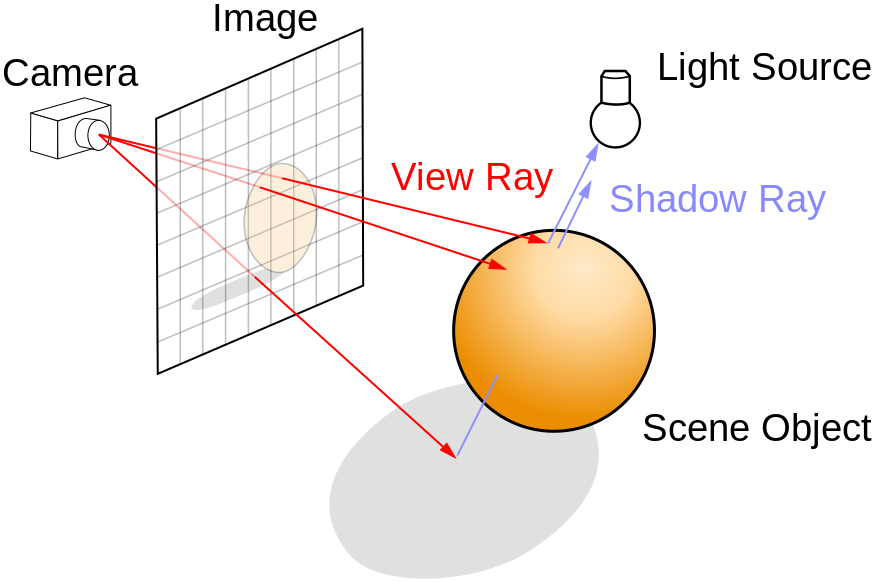
\includegraphics[scale=0.35]{media/Ray_trace_diagram.png}
	\caption{\textit{Ray Casting} algorithm overview. Source: Ray tracing (graphics), Wikipedia}
	\label{globalilum}
\end{figure}

Ray tracing uses this mechanism to recursively accumulate the light contribution from reflective and refractive objects. Materials like mirrors or polished metals produce a reflection ray, and transparent or glass objects may produce both reflection and refractive rays. This process occurs recursively, which each new ray may generate new both reflective and refractive rays. Recursion has some cut-off limit, such as a maximum number of bounces (depth). Moreover, the recursion ends when the ray hits a light source or leaves the scene. The number of bounces affects directly to the resultant image. In Figure \ref{bounces}, we can see how the more bounces, the more reflections appear in the rendered image.

\begin{figure}[H]
	\centering
	\medskip
	\begin{subfigure}{.48\textwidth}
		\centering
		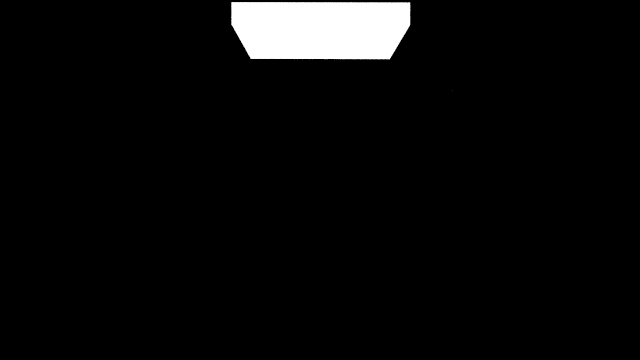
\includegraphics[scale=0.315]{media/mirrors_rect/cornell_mirrors_1.png}
		\caption{1 bounce per ray}
		\label{mr_rect_1}
	\end{subfigure}
	\begin{subfigure}{.48\textwidth}
		\centering
		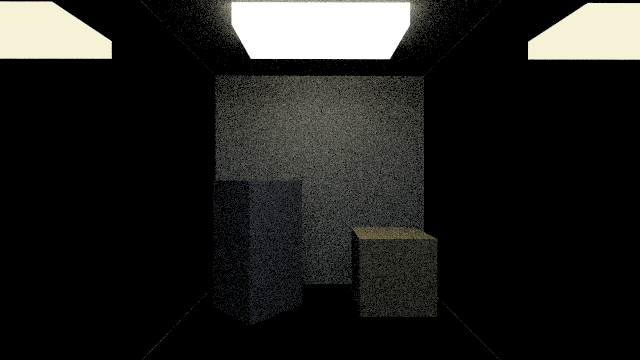
\includegraphics[scale=0.315]{media/mirrors_rect/cornell_mirrors_2.png}
		\caption{2 bounces per ray}
		\label{mr_rect_2}
	\end{subfigure}
	
	\medskip
	\begin{subfigure}{.48\textwidth}
		\centering
		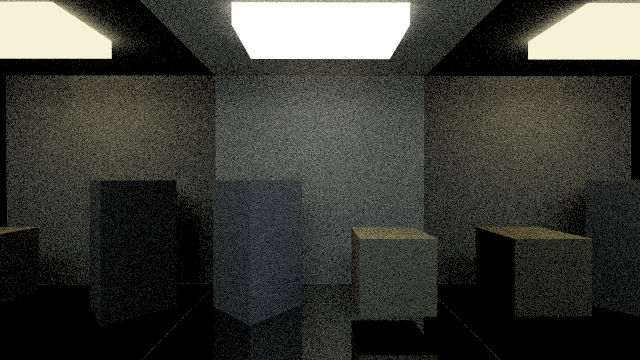
\includegraphics[scale=0.315]{media/mirrors_rect/cornell_mirrors_3.png}	
		\caption{3 bounces per ray}
		\label{mr_rect_3}
	\end{subfigure}		
	\begin{subfigure}{.48\textwidth}
		\centering
		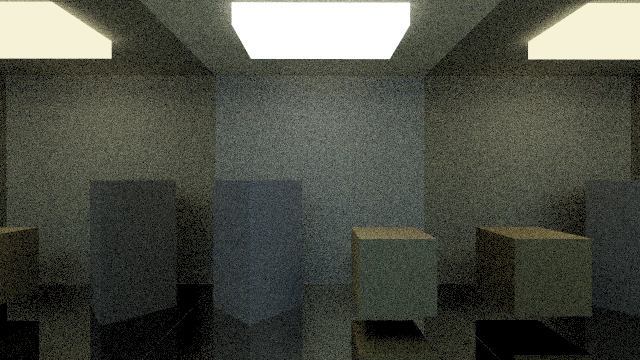
\includegraphics[scale=0.315]{media/mirrors_rect/cornell_mirrors_4.png}
		\caption{4 bounces per ray}
		\label{mr_rect_4}
	\end{subfigure}
	
	\medskip	
	\begin{subfigure}{.48\textwidth}
		\centering
		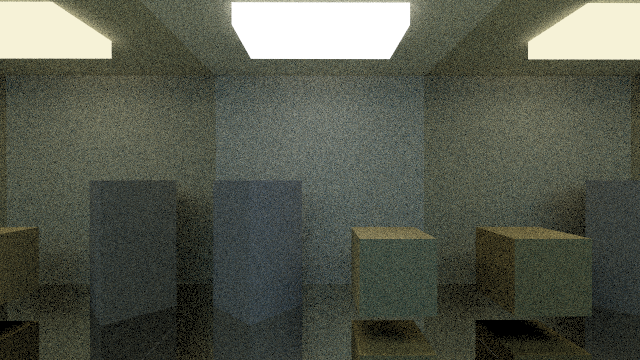
\includegraphics[scale=0.315]{media/mirrors_rect/cornell_mirrors_5.png}
		\caption{5 bounce per ray}
		\label{mr_rect_5}
	\end{subfigure}
	\begin{subfigure}{.48\textwidth}
		\centering
		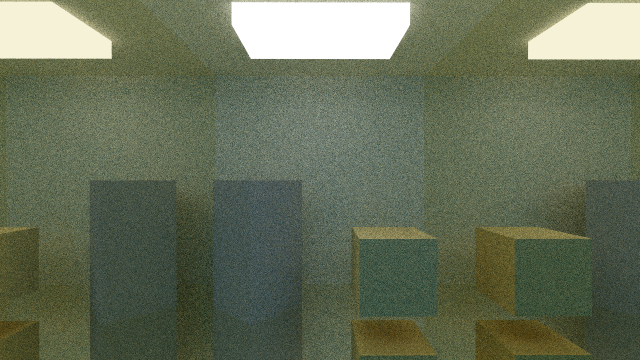
\includegraphics[scale=0.315]{media/mirrors_rect/cornell_mirrors_20.png}	
		\caption{20 bounce per ray}
		\label{mr_rect_20}
	\end{subfigure}
	\caption{Reflections increase with the numbers of bounces.}
	\label{bounces}
\end{figure}

To simulate the global illumination of a scene we have to consider how the light interacts through the scene. To do this we must solve the equation of light transport, described by Kajiya \citep[pp.~143--150]{Kajiya1986}. This function approximates the radiance of a given pixel by simulating the paths of light through the sum of self-emitted radiance and reflected radiance. This result is distributed according to the \textit{bidirectional reflectance distribution function} (BRDF) defined in the material, as we will see later. That BRDF varies according to the type of material because light does not behave the same way when it hits a diffuse material as it does when it hits a mirror or glass type material.

\begin{figure}[!ht]
	\centering
	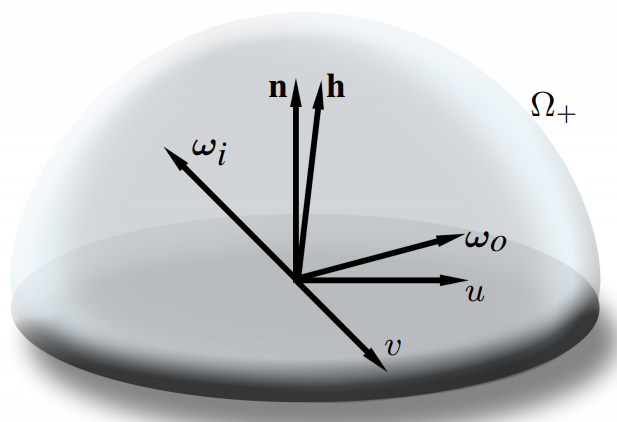
\includegraphics[scale=0.35]{media/Rendering_eq.png}
	\caption{Hemisphere scheme. Source: \citep{Kurt2010}}
	\label{rendeq}
\end{figure}

\begin{equation}
\begin{split}
L_o(x,\omega_o,\lambda,t) & = L_e(x,\omega_o,\lambda,t) + L_r(x,\omega_i,\omega_o,\lambda,t)L_i(x,\omega_i,\lambda,t) \\
L_o(x,\omega_o,\lambda,t) & = L_e(x,\omega_o,\lambda,t) + \int_\Omega f_r(x,\omega_i,\omega_o,\lambda,t)L_i(x,\omega_i,\lambda,t)(\omega_i \cdot n) d\omega_i
\end{split}
\end{equation}

The integral for the reflected light is calculated over the hemisphere in all possible directions. Calculating all directions is impossible, which is why it is approximated by Monte Carlo. The integral is converted into a finite sum of samples. The main problem with approximating the equation by Monte Carlo is that it produces images with a lot of noise. So for each pixel, a number $n$ of samples is used and the final value is its average. This is known as supersampling.

\subsection{Supersampling}

Supersampling is a method of anti-space aliasing. This method aims to minimize aliasing, an effect that causes continuous signals, such as the image, to be indistinguishable. 

In our field, computer graphics, anti-aliasing aims to smooth the edges of objects in a scene. This implies a higher performance cost as we need to perform more calculations for each pixel.

There are different patterns of supersampling, the simplest of which is the grid pattern. In this method, if we want to calculate the value of a pixel (i,j) we divide it into 'n' sub-pixels and the final result will be the average of these sub-pixels. Another quite common pattern, and the one we use in our project, is the random (or stochastic) one. In this case for a given pixel (i,j) we take 's' sub-pixels from its surroundings at random.

\begin{figure}[!ht]
	\centering
	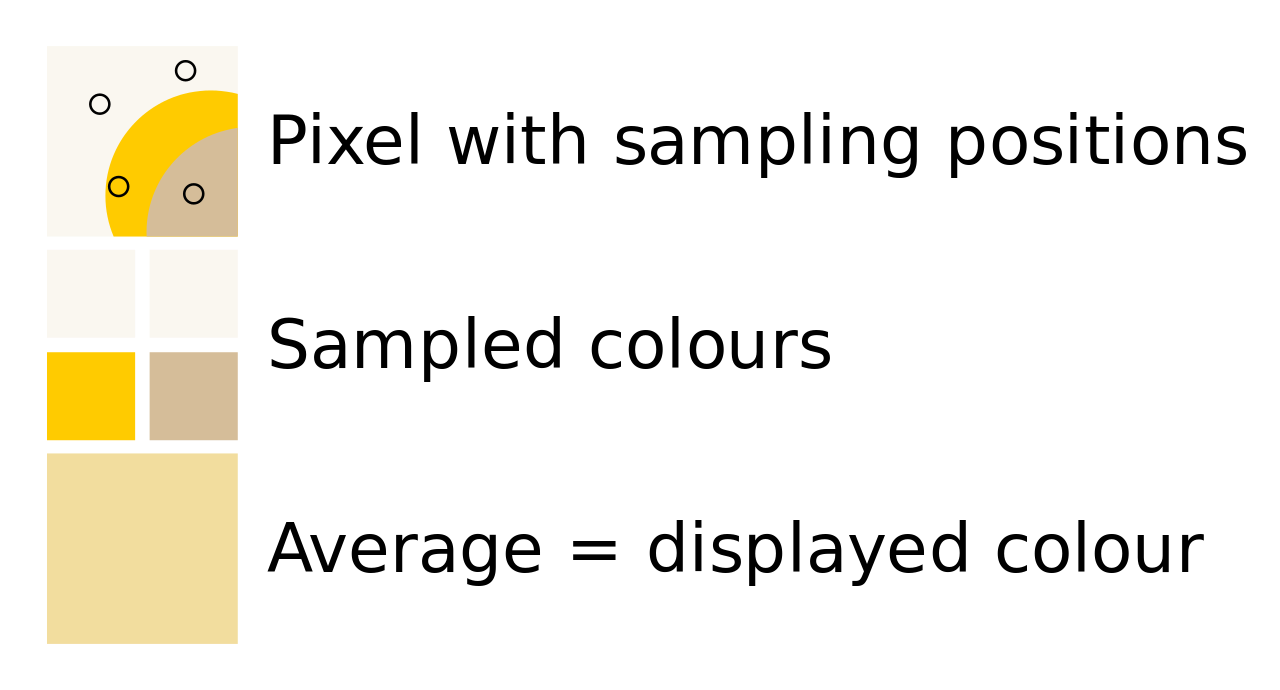
\includegraphics[scale=0.20]{media/Supersampling.png}
	\caption{Example of supersampling for one pixel: \citep{Kurt2010}}
	\label{SA}
\end{figure}

\section{What is a ray?}

A ray is just a three-dimensional line that is usually specified as an interval between an origin and a destination, two three-dimensional points $A$ and $B$. Unlike a line in two dimensions, $y = m x + b$, there is no explicit way to define a three-dimensional line. So we need a parametric function that allows us to move along this line. We can represent this function as a weighted average of points $A$ and $B$:

\begin{equation}
P(t) = (1-t)A + tB
\end{equation}

Where $t$ can take any real value, $t \in [-\infty, \infty]$. But it is more common, and for a rendering algorithm it is preferable, to use a point and a direction vector rather than two points. Because, in essence, in this type of algorithm you're "throwing" rays in one direction. So, the follow representation is more common:

\begin{equation} \label{rayeq}
P(t) = O + tD
\end{equation}

Where $O$ is the origin point, for example the camera, and $D$ is the direction.

\section{Camera}

The camera is the entity that defines how we will see the scene. To define a camera we need its position in world space, the direction it is facing, a vector pointing to the right and a vector pointing upwards from the camera. 

\begin{figure}[!ht]
	\centering
	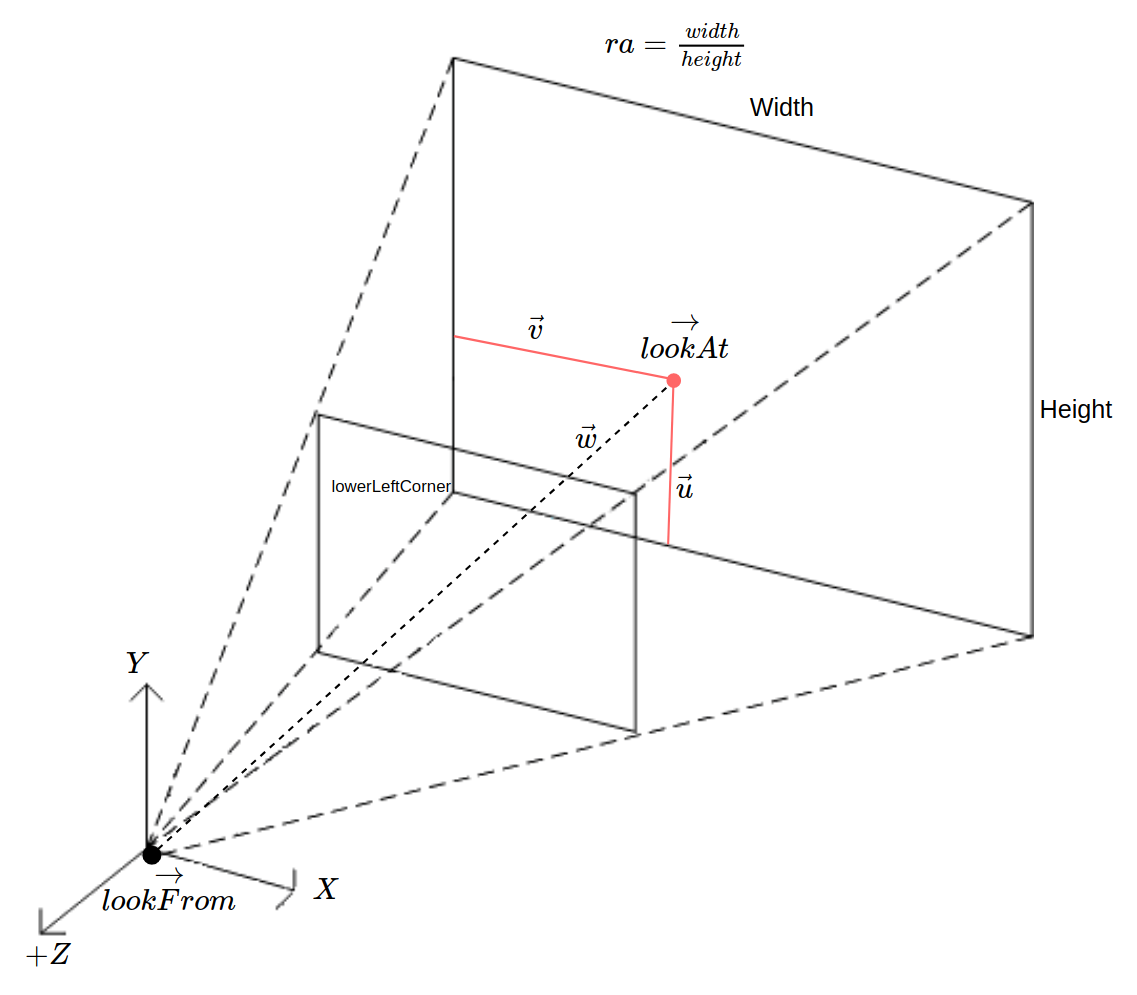
\includegraphics[scale=0.35]{media/camera.png}
	\caption{Camera geometry.}
	\label{camegeom}
\end{figure}

The up vector can have another direction, but it will make us see the scene rotated. In Figure \ref{cameraup} we can see how the resulting image varies according to the definition of the vector up.

\begin{figure}[H]
	\centering
	\medskip
	\begin{subfigure}{.48\textwidth}
		\centering
		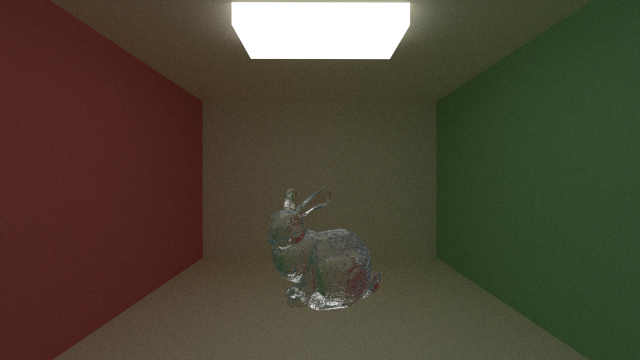
\includegraphics[scale=0.35]{media/cornell_bunny.png}
		\label{cameraupy}
	\end{subfigure}
	\begin{subfigure}{.48\textwidth}
		\centering
		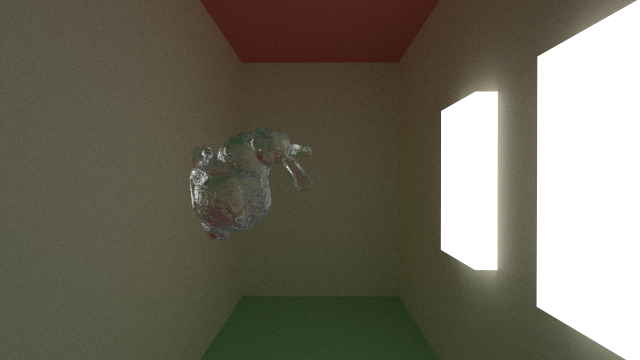
\includegraphics[scale=0.35]{media/cornell_bunny_z_1.png}
		\label{cameraupz}
	\end{subfigure}
	
	\caption{Vector up $(0,1,0)$ (top) and $(0,0,1)$ (bottom).}
	\label{cameraup}
\end{figure}

\subsubsection{Camera position - $\vec{lookFrom}$}

The position of the camera is defined by a vector, $\vec{lookFrom}$, in world space that points to the camera position. The position of the camera is defined by a vector in world space that points to the camera position. The scene in Figure \ref{cameraup}, for example, has the position set to $(12 0.05 0.05)$.

\subsubsection{Camera direction - $\vec{w}$}

To determine the direction vector, $\vec{w}$, we need the position vector, $\vec{lookFrom}$, and a target vector. This target vector, $\vec{lookAt}$, is where the camera looks and represents the centre of the canvas. We can define the direction as:

\begin{equation}
\vec{w} = \frac{\vec{lookFrom} - \vec{lookAt}}{||\vec{lookFrom} - \vec{lookAt}||}
\end{equation}

\subsubsection{Right axis - $\vec{u}$}

The right vector, $u$, represents the positive $x$-axis in camera space. This vector can be obtained from the cross product of up vector and $w$ vector.

\begin{equation}
\vec{u} = \frac{\vec{lookFrom} \times \vec{lookAt}}{||\vec{lookFrom} \times \vec{lookAt}||}
\end{equation}

\subsubsection{Up axis - $\vec{v}$}

To get this vector, we only need to do the cross product between $\vec{w}$ and $\vec{u}$. 

\begin{equation}
\vec{v} = \vec{w} \times \vec{u}
\end{equation}

\subsubsection{Image plane}

Once we have all the vectors, we can calculate the lower left corner to obtain the image plane (canvas). We will use this value to move through the frustum to throw the rays.

The set of vectors $e_1 = (1,0,0)$, $e_2 = (0,1,0)$ and $e_3 = (0,0,1)$ form between them an orthogonal basis of $\mathbb{R}^3$. So all the vectors $(x,y,z)$ in $\mathbb{R}^3$ can be expressed as the sum of the base vectors:

\begin{equation}
(x,y,z) = xe_1 + ye_2 + ze_3
\end{equation}

Then we can define the lower left corner as:

\begin{equation}
lfc = origin - half\_width e_1 - half\_heigth e_2 - e_3
\end{equation}

\begin{figure}[!ht]
	\centering
	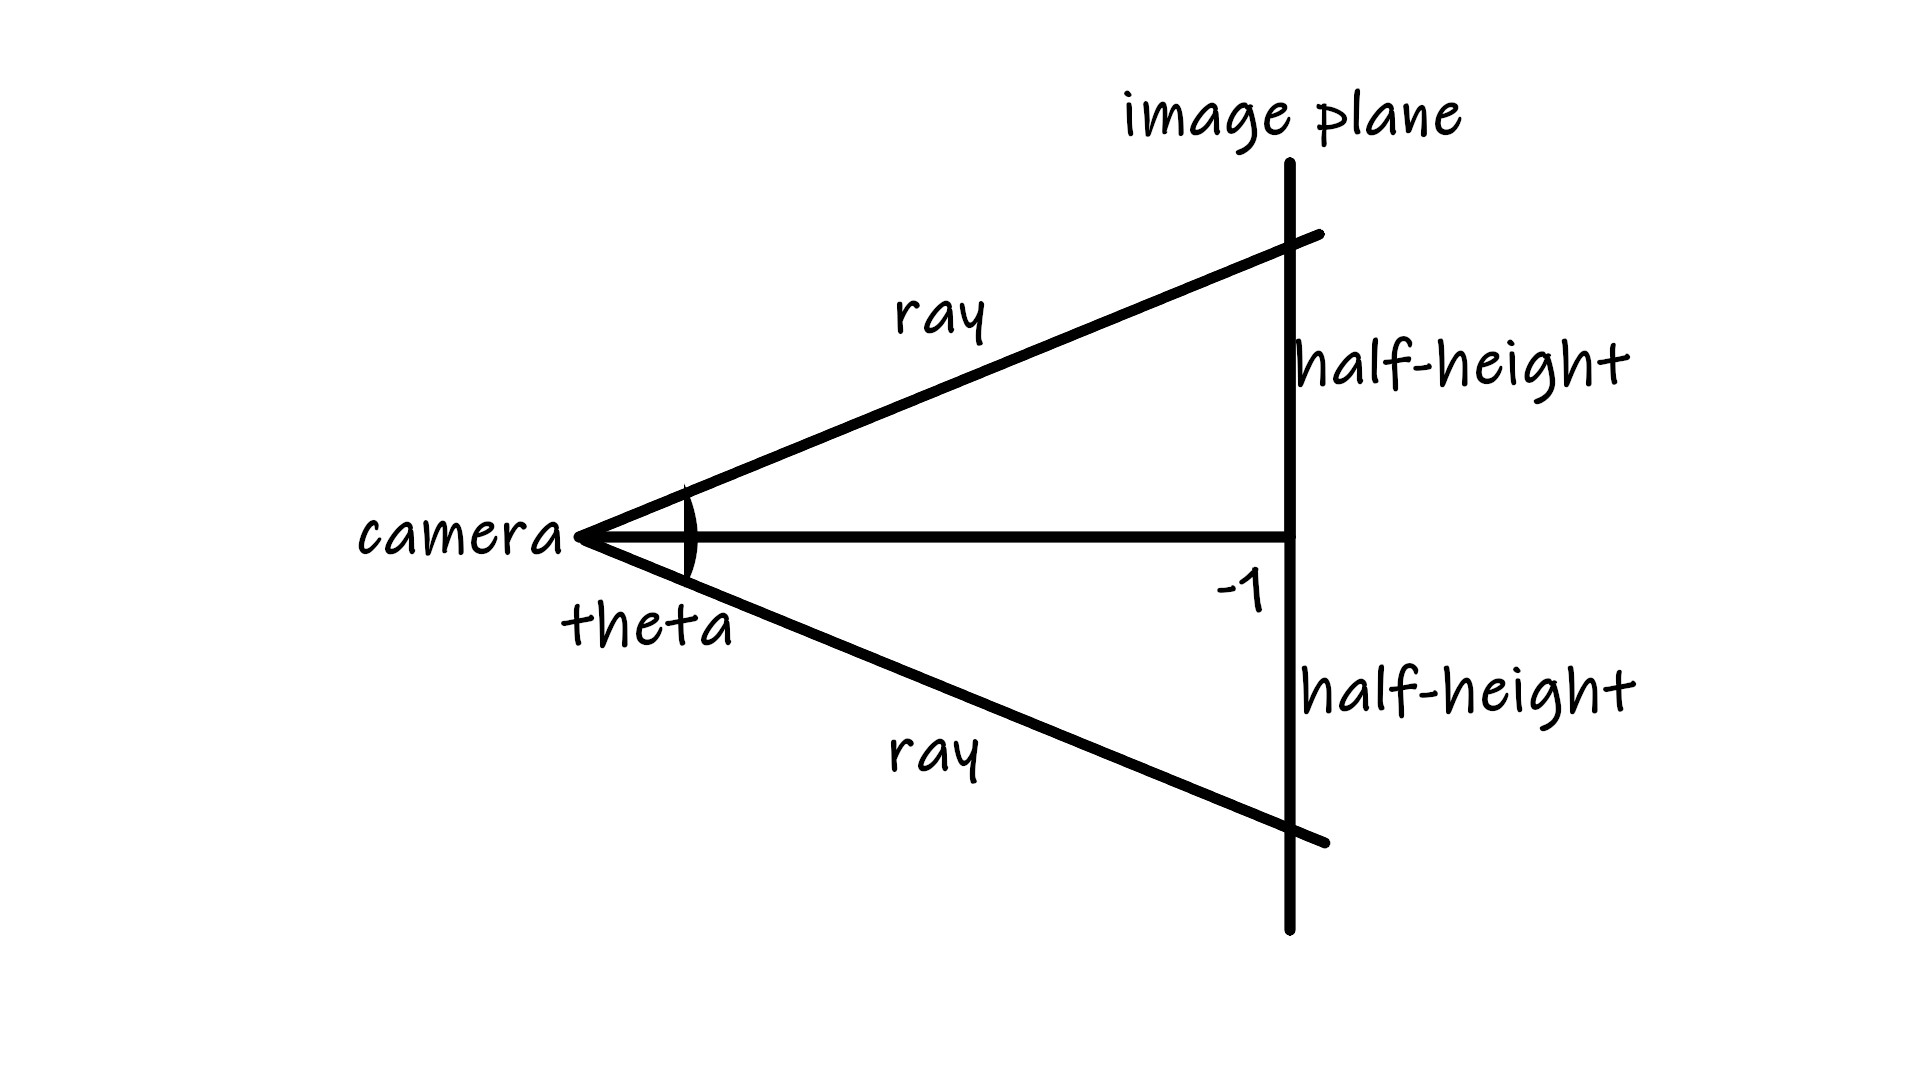
\includegraphics[scale=0.65]{media/camera-model-summary-0.jpg}
	\caption{Camera geometry.}
	\label{camegeom2}
\end{figure}

Looking the Figure \ref{camegeom2}, if the open angle of camera lens is $\theta$, then $half\_height = tan(\frac{\theta}{2})$. The theta angle is given by the camera's field of view (FOV). By convention the FOV is stipulated in degrees, but to perform the calculations we must make a conversion to radians, so $\theta = \frac{FOV \pi}{180}$.

The vectors u,v and w are a projection of the $x$, $y$ and $z$-axes respectively, so we can use them as a basis for the calculation of the lower left corner. Then, the equation to find it would look like this:

\begin{equation}
lfc = origin - half\_width v - half\_heigth v - w
\end{equation}

\subsubsection{Defocus blur}

Defocus Blur, commonly called Depth of Field, is an effect caused by cameras in which objects farther away from the lens are blurred. The Defocus Blur can be calculated from the focal length, the circle of confusion and the aperture.

\begin{figure}[!ht]
	\centering
	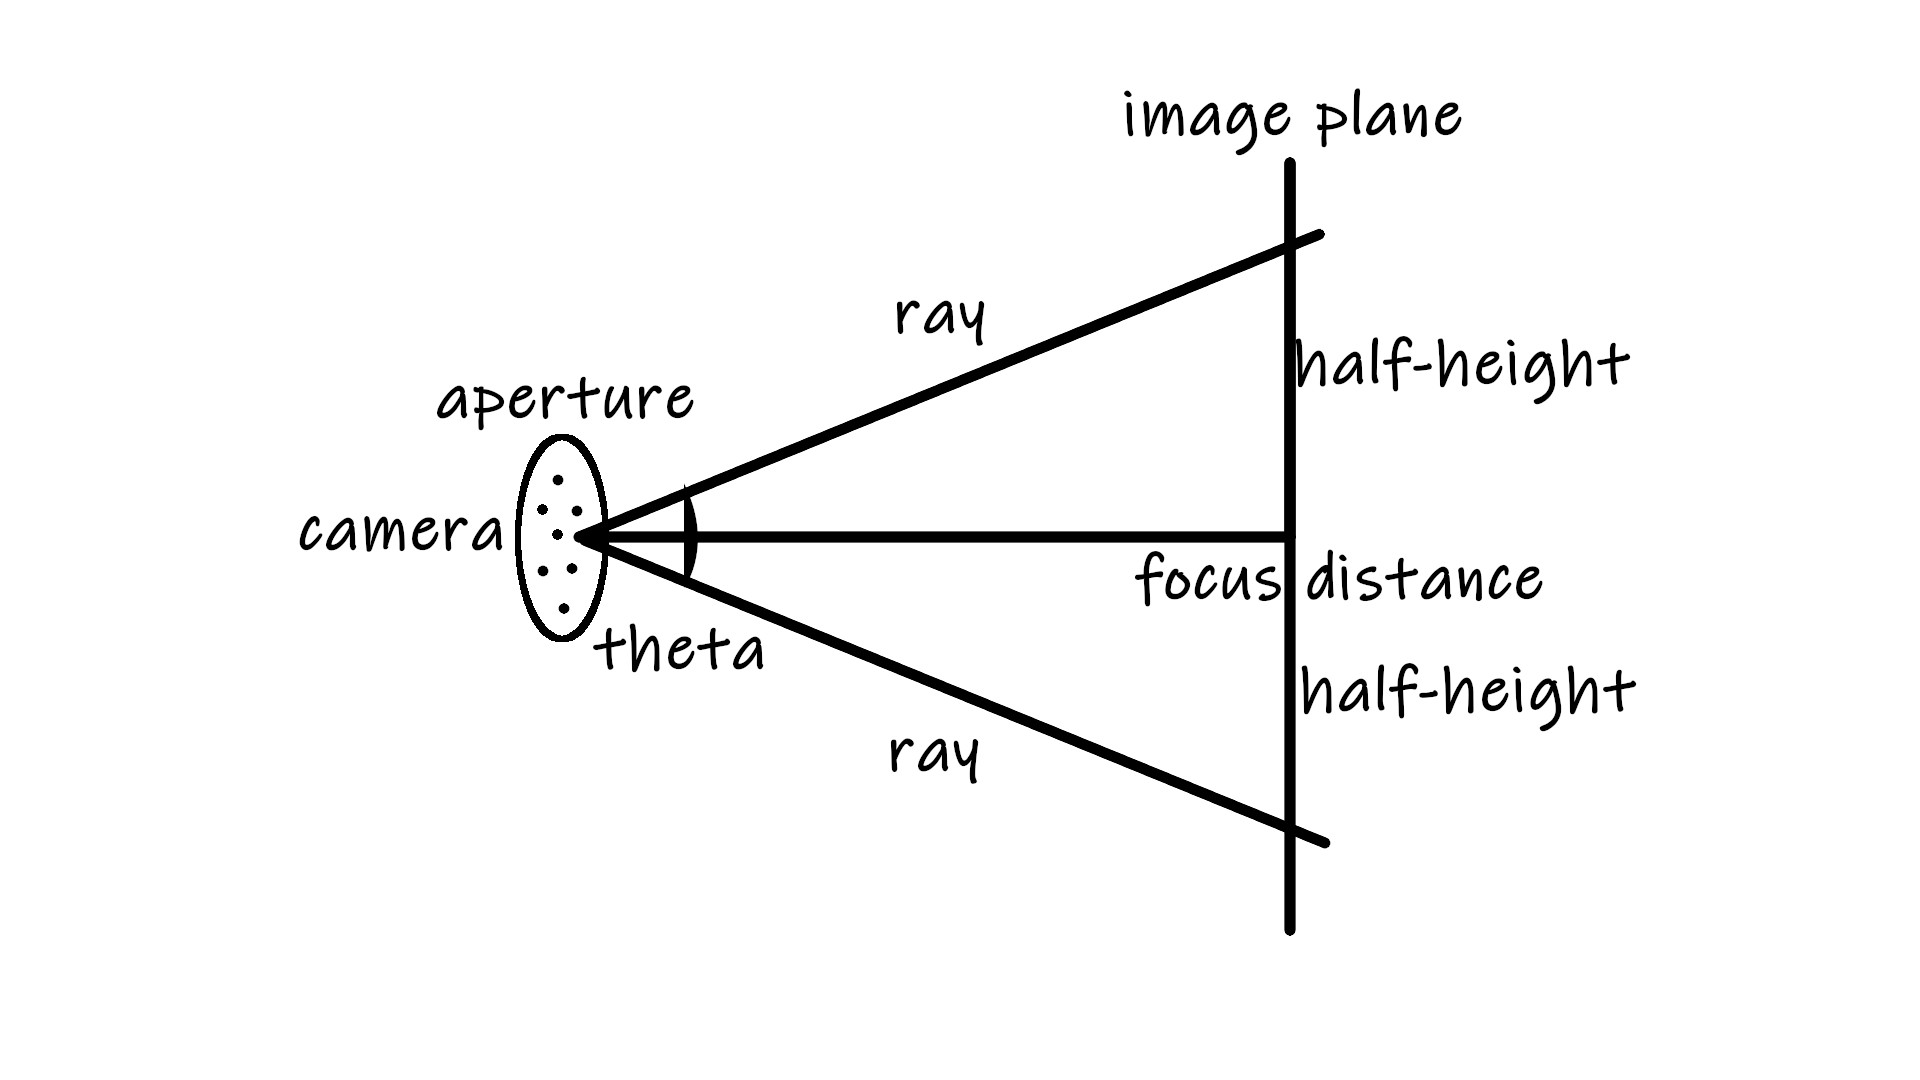
\includegraphics[scale=0.65]{media/camera-model-summary-2.jpg}
	\caption{Camera geometry.}
	\label{camegeom3}
\end{figure}

To add this effect we must multiply $half\_height$ by the focal length. Also, when we generate a ray we will add an offset calculated from the radius of the lens (half of the aperture) and the circle of confusion. If we have no blur, all ray are originated at the disk center($\vec{lookFrom}$).

By experimenting with the aperture value and the focal length, we can obtain results like those shown in Figure \ref{dof}. Also, we can see how the aperture affects at the total illumination captured by the camera.

\begin{figure}[H]
	\centering
	\medskip
	\begin{subfigure}{.48\textwidth}
		\centering
		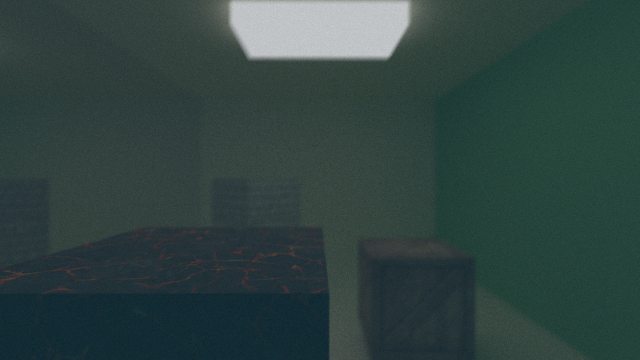
\includegraphics[scale=0.315]{media/cornell_textures_dof_1.png}
		\caption{Background of image blurred.}
		\label{dof1}
	\end{subfigure}
	\begin{subfigure}{.48\textwidth}
		\centering
		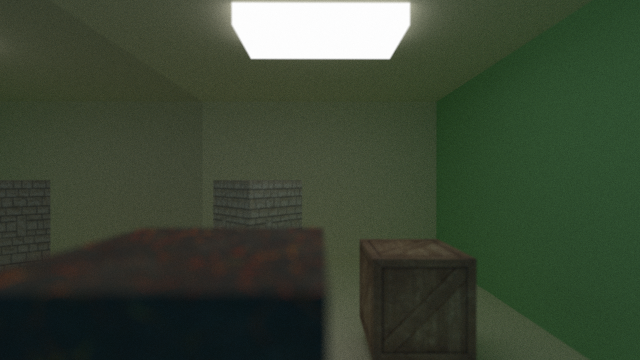
\includegraphics[scale=0.315]{media/cornell_textures_dof_2.png}
		\caption{Front of image blurred.}
		\label{dof2}
	\end{subfigure}
	
	\medskip
	\begin{subfigure}{.98\textwidth}
		\centering
		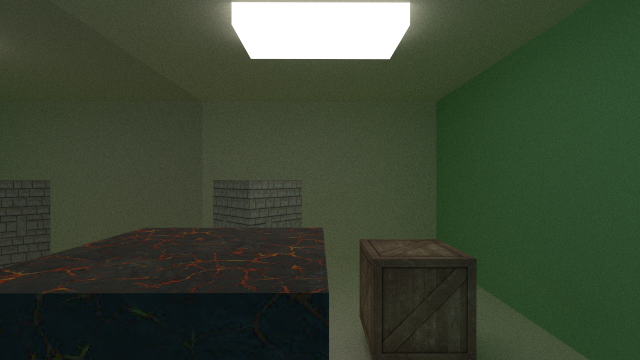
\includegraphics[scale=0.65]{media/cornell_textures_dof_3.png}	
		\caption{Non blurred image.}
		\label{dof3}
	\end{subfigure}
	\caption{Scene rendered experimenting with focus length and aperture of the camera.}
	\label{dof}
\end{figure}

We use an aperture of 0.5 in both Figures, \ref{dof1} and \ref{dof2}. But in Figure \ref{dof1} we set the focus length as $\frac{|(\vec{lookFrom}-\vec{lookAt})|}{6}$. Having a length of focus close to the camera lens causes the background of the image to be blurred and also catches less light. On the other hand, in Figure \ref{dof2}, we have put the focus length closer to the centre of the scene so that what is closer to the camera is blurred, thus focusing on the background.

Finally, we can see in Figure \ref{dof} how it is the result of an image where the rays that come out of the centre of the circle of confusion, so they are centred in the origin of the camera and there is no blurring.

\section{Triangles}

For this project, we will have only one shape to represent the objects in the scene: Triangles. We choose triangles because with them we can represent 3D models. As we said in the first chapter, the triangle is the most common shape to represent a 3D model.

As we commented in the introduction of the project, we have a version that uses a BVH and another one that does not. For both, each triangle has three vertices that represent their position in the scene, three texture coordinates, his centroid and the material assigned. Also, for the BVH version, it has the bounding box and a Morton code, later in the section about the implemented BVH we will explain what this code is for.

\subsection{Collision detection}

To detect collisions, we must use some type of bounding volume that allows us to query if a ray has hit an object. These bounding volume can go to primitive scale, lower level, or 3D model scale. For our project, we have decided to implement it at the primitive level which implies a higher cost because the BVH that we generate will be much deeper, but we will also have a better quality in terms of calculation of accurate collisions. Also, as we are performing an offline rendering algorithm, the time that this strategy can add to the algorithm is not critical. There are three main types of colliders: Bounding Sphere, Axis-Aligned Bounding Box and Oriented Bounding Box. But we have other shapes like cylinder, ellipsoid, capsule, convex hull, etc. For this project we have decided to use the Axis-Aligned Bounding Box (AABB).

\begin{figure}[!ht]
	\centering
	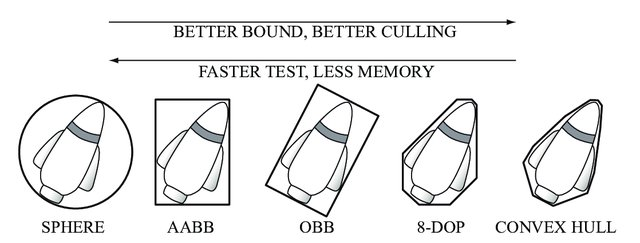
\includegraphics[scale=1.25]{media/volumes.jpg}
	\caption{Bounding volumes shapes. Source: \citep[pp.~236–237]{Ericson2004}}
	\label{BV}
\end{figure}


An AABB or an OBB is a cuboid (in 3D) or a rectangle (in 2D) that contains the object or its primitives. In the case of an AABB, it is aligned with the scene coordinate system while an OBB is aligned with the local coordinate system of the object. AABBs are aligned with the scene coordinate system, so it is easier to perform intersection tests. But in case we rotate an object we must recompute its bounding box.

\subsection{Axis-Aligned Bounding Box intersection algorithm}

Before calculating the ray-triangle intersection, we must see if the ray has hit the bounding volume. One of the most commonly used algorithms is the slab algorithm. The axis-aligned bounding box can only be represented by two 3D points: $(x_{min},y_{min},z_{min})$ and $(x_{max},y_{max},z_{max})$. With these two points, we can reconstruct the cuboid in a very simple way. 

To understand how the slab method works, let's see how it works in two dimensions, because in three dimensions it behaves the same way but instead of having lines we have planes.

\begin{figure}[!ht]
	\centering
	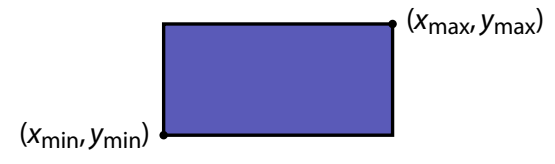
\includegraphics[scale=0.5]{media/slab_1.png}
	\caption{2D Bounding box}
	\label{AABB1}
\end{figure}

If we throw a ray ($R(t) = O + tD$), we will have a hit if the ray intersects with both axes $(x,y)$.

\begin{figure}[!ht]
	\centering
	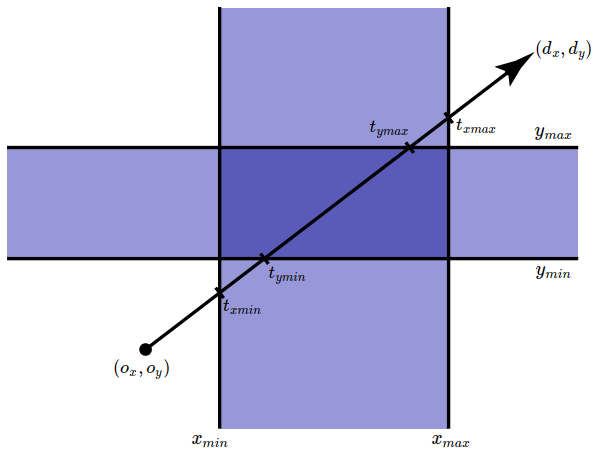
\includegraphics[scale=0.5]{media/slab_2.png}
	\caption{Ray-box intersection}
	\label{AABB2}
\end{figure}

From the equation \ref{rayeq}, we know that $x_{min} = O_x + t_{xmin} D_x$ and $y_min = O_y + t_{ymin} D_y$. We know all the values except for $t_{xmin}$ and $t_{ymin}$. So finally we have the following equations.

\begin{equation} \label{slab_method_1}
\begin{split}
t_{xmin} & = \frac{x_{min - O_x}}{D_x} \\
t_{ymin} & = \frac{y_{min - O_y}}{D_y} \\
\\
t_{max} & = \frac{x_{max - O_x}}{D_x} \\
t_{max} & = \frac{y_{max - O_y}}{D_y} \\
\end{split} 
\end{equation}

We can define the following vectors:

\begin{equation} \label{slab_method_2}
\begin{split}
t_{0} & = \left( \frac{x_{min - O_x}}{D_x}, \frac{y_{min - O_y}}{D_y} \right) \\
\\
t_{1} & = \left( \frac{x_{max - O_x}}{D_x}, \frac{y_{max - O_y}}{D_y} \right) \\
\end{split} 
\end{equation}

If we stop here, we may have a problem in case the lightning has a negative direction. We can solve this by taking the minimum and maximum of both resulting vectors. So we will define two vectors $t_{min}$ and $t_{max}$:

\begin{equation} \label{slab_method_3}
\begin{split}
t_{smaller} & = min(t_0, t_1) \\
\\
t_{bigger} & = max(t_0, t_1) \\
\end{split} 
\end{equation}

When we launch a primary ray, those that come out of the camera, the interval in which it moves is $[-\infty, \infty]$. To find out if the ray has hit the bounding box, we have to see that $t_{min} < t_{max}$, that means that the hit point is inside the bounding box. The value of $t_{min}$ can be obtained by taking the maximum value with the $t_{min}$ that receives the function, and $t_{xmin}$ and $t_{ymin}$. In the same way for $t_{max}$ but taking the minimum value. This is the implementation for the ray-AABB intersection test.

\begin{algorithm}[caption={collision}]
input: Ray $r$, float tmin, float tmax
output: boolean
begin
  $Vector_3 (i_x, i_y, i_z) = \frac{(1,1,1)}{(D_x, D_y, D_z)}$
  
  $Vector_3 t_0 = ((min_x, min_y, min_z) - (O_x, O_y, O_z)) (i_x, i_y, i_z)$
  $Vector_3 t_1 = ((max_x, max_y, max_z) - (O_x, O_y, O_z)) (i_x, i_y, i_z)$

  $Vector_3$ $t_{smaller}$ = min($t_0$, $t_1$)
  $Vector_3$ $t_{bigger}$ = max($t_0$, $t_1$)
  
  tmin = max(tmin, max(${t_{smaller}}_x$, max(${t_{smaller}}_y$, ${t_{smaller}}_z$)))
  tmax = min(tmax, min(${t_{bigger}}_x$, min(${t_{bigger}}_y$, ${t_{bigger}}_z$)))
  
  return tmin $<$ tmax
end
\end{algorithm}

\subsection{Möller–Trumbore intersection algorithm}

In order to calculate the intersection of a ray and triangle, we will use the Möller–Trumbore algorithm. We choose this algorithm because, as the authors say in their publication \citep{Moller2005}, uses minimal storage. We only have to know the vertices $(V_0,V_1,V_2)$ to test the intersection.

Previous algorithms have solved this intersection test by solving first the intersection between the plane where the triangle lies and then test if the ray is inside the triangle. In Möller–Trumbore, a transformation is applied to the ray, and we avoid the intersection ray/plane.

A point, $T(u,v)$, on a triangle, where $(u,v)$ are the barycentric coordinates and $u,v \geq 0$ and $u+v \leq 1$, is given by:

\begin{equation} \label{barycentric}
\begin{split}
T(u,v) & = (1-u-v)V_0 + uV_1 + vV_2 \\
T(u,v) & = V_0 - uV_0 - vV_0 + uV_1 + vV_2 \\
T(u,v) & = V_0 + u(V_1 - V_0) + v(V_2 - V_0)
\end{split}
\end{equation}

Also, the point $(u,v)$ can be used for texture mapping, color interpolation etc. Computing the intersection between the ray, $R(t)$, and the triangle, $T(u,v)$, is equivalent to $R(t) = T(u,v)$. In the last section, we define a ray as $R(t) = O + t D$. So, we need to solve the following equation:

\begin{equation}
\begin{split}
O + tD & = V_0 + u(V_1 - V_0) + v(V_2 - V_0) \\
O - V_0 & = -tD + u(V_1 - V_0) + v(V_2 - V_0)
\end{split}
\end{equation}

On the right side of the equation, we have three unknown variables $(t,u,v)$ multiplied by three known therms $(D, V_0V_1, V_0V_2)$. We can rearrange this equation in a vector form and we get:

\begin{equation}
\begin{bmatrix}
-D & \left(V_1 - V_0\right) & \left(V_2 - V_0\right)
\end{bmatrix}
\begin{bmatrix}
t \\ u \\ v
\end{bmatrix}
= O - V_0
\end{equation}

We only have to solve the following linear equations system using Cramer's rule. Consider a system of $n$ linear equations for $n$ unknowns therms represented as $MX = C$. If the multiplication of a matrix $M$ ($\left[-D, \left(V_1 - V_0\right), \left(V_2 - V_0\right)\right]$ in our case) by a column vector $X$ ($\left[t,u,v\right]^T$ ) is equal to a column vector $C$, then it's possible to find $X_i$ (the $i$-th element of vector $X$) as follows: 

\begin{equation}
x_i = \frac{det(M_i)}{det(A)}
\end{equation}

where $M_i$ is the matrix formed by replacing the $i$-th column of $M$ by the column vector $C$ ($O - V_0$ in our case). Then, using Cramer's rule we get:

\begin{equation}
\begin{bmatrix}
t \\ u \\ v
\end{bmatrix}
=
\frac{1}{\left[|-D, \left(V_1 - V_0\right), \left(V_2 - V_0\right)|\right]}
\begin{bmatrix}
| \left(0 - V_0\right) & \left(V_1 - V_0\right) & \left(V_2 - V_0\right) | \\
| -D & \left(0 - V_0\right) & \left(V_2 - V_0\right) | \\
| -D & \left(V_1 - V_0\right) & \left(0 - V_0\right) | \\
\end{bmatrix}
\end{equation}

We can denote $\left(V_1 - V_0\right)$ as $E_1$, $\left(V_2 - V_0\right)$ as $E_2$ and $\left(O - V_0\right)$ as $T$ to make the equation more readable. So, we get:

\begin{equation} \label{cramer}
\begin{bmatrix}
t \\ u \\ v
\end{bmatrix}
=
\frac{1}{\left[|-D, E_1, E_2|\right]}
\begin{bmatrix}
|  T & E_1 & E_2 | \\
| -D & T & E_2 | \\
| -D & E_1 & T | \\
\end{bmatrix}
\end{equation}

We know that $|A, B, C| = -\left( A \times C \right) \cdot B = -\left( C \times B \right)\cdot A$, whether $A$,$B$ and $C$ are vectors, then equation \ref{cramer} could be rewritten as:

\begin{equation} \label{cramer2}
\begin{bmatrix}
t \\ u \\ v
\end{bmatrix}
=
\frac{1}{\left[\left( D \times E_2 \right) \cdot E_1 \right]}
\begin{bmatrix}
\left( T \times E_1 \right) \cdot E_2 \\
\left( D \times E_2 \right) \cdot T \\
\left( T \times E_1 \right) \cdot D \\
\end{bmatrix}
\end{equation}

Denote $P = \left( D \times E_2 \right) $ and $Q = \left( T \times E_1 \right)$ then, we get:

\begin{equation}
\begin{split}
t & = \frac{1}{P \cdot E_1} \left(Q \cdot E_2 \right) \\
u & = \frac{1}{P \cdot E_1} \left(P \cdot T \right) \\
v & = \frac{1}{P \cdot E_1} \left(Q \cdot D \right) \\
\end{split}
\end{equation}

\section{Geometric transforms}

To be able to place an object in the position of the scene we want, it is necessary to apply a series of basic geometric transformations that allow us to do it. In addition, it is possible that many models have a different coordinate system from ours. Therefore, we must accurately handle them to be able to visualize them. That's why for each of the models we must calculate the centre of it, in order to bring it to the centre of the coordinate system of the scene and thus be able to manage it properly.

The geometric transformations we can make to the models are translation, rotation and scaling. For all of them, we will use a homogeneous coordinate system to represent them by means of a space vector multiplied by the appropriate matrix. If we want to apply some transformation $T$ to a  vector $p = (p_x, p_y, p_z)$, we rewrite $p$ using four homogeneous coordinates as $p = (p_x, p_y, p_z, 1)$.

\subsection{Translation}

If we want to move an object $O$ by a vector $t = (t_x, t_y, t_z)$, then we need to add $t$ to the set of vertices $V$ from $O$.

\begin{equation}
\{\forall v \in V | v + t\}
\end{equation}

It is better to perform these transformations in matrix notation, because if we want to apply more than one transformation to an object we simply have to perform matrix multiplications. Therefore, we must multiply each vertex by the following matrix.

\begin{equation}
T_v = 
\begin{bmatrix}
1 & 0 & 0 & t_x \\
0 & 1 & 0 & t_y \\
0 & 0 & 1 & t_z \\
\end{bmatrix}
\end{equation}

By convention, it is common to use a homogeneous coordinate system, so we will have to add a fourth coordinate w to each vertex.

\begin{equation}
\{\forall v \in V | v = (v_x, v_y, v_z) \rightarrow (v_x, v_y, v_z, 1)\}
\end{equation}

Then we have to add a new row to the matrix with the homogeneous coordinate. We have the following matrix.

\begin{equation}
T_t = 
\begin{bmatrix}
1 & 0 & 0 & t_x \\
0 & 1 & 0 & t_y \\
0 & 0 & 1 & t_z \\
0 & 0 & 0 & 1 \\
\end{bmatrix}
\end{equation}

For each vertex we multiply it by the matrix $T_t$.

\begin{equation}\label{translate}
T_t v = 
\begin{bmatrix}
1 & 0 & 0 & t_x \\
0 & 1 & 0 & t_y \\
0 & 0 & 1 & t_z \\
0 & 0 & 0 & 1 \\
\end{bmatrix}
\begin{bmatrix}
v_x \\
v_y \\
v_z \\
1 \\
\end{bmatrix}
=
\begin{bmatrix}
v_x + t_x \\
v_y + t_y \\
v_z + t_z \\
1 \\
\end{bmatrix}
= v + t
\end{equation}

\subsection{Scaling}

The scaling is very similar to the translation, but instead of adding the scaling vector $s = (s_x, s_y, s_z)$ to the set of vertices $V$ of the object, it has to be multiplied.

\begin{equation}
\{\forall v \in V | v s\}
\end{equation}

We define scaling as a vector s, because sometimes we may not want uniform scaling on all axes. As with translation, we will define the scaling with a scaling matrix $S_s$ with a homogeneous coordinate system.

\begin{equation}\label{scaling}
T_t v = 
\begin{bmatrix}
S_x & 0 & 0 & 0 \\
0 & S_y & 0 & 0 \\
0 & 0 & S_z & 0 \\
0 & 0 & 0 & 1 \\
\end{bmatrix}
\begin{bmatrix}
v_x \\
v_y \\
v_z \\
1 \\
\end{bmatrix}
=
\begin{bmatrix}
v_x s_x \\
v_y s_y \\
v_z s_z \\
1 \\
\end{bmatrix}
= v s
\end{equation}

\subsection{Rotation}

In the rotation, we have three axes in which we can rotate the object, the $x$, $y$ and $z$-axis. The most basic rotation only uses one of these axes, so we can define a rotation matrix for each of the axes. The following matrices rotate a vector $v$ by an angle $\theta$ in the $x$, $y$ and $z$-axes using the right-hand rule (all matrices represent a clockwise rotation).

\begin{equation}\label{rotx}
R_x = 
\begin{bmatrix}
1 & 0 & 0 & 0 \\
0 & cos\theta_x & -sin\theta_x & 0 \\
0 & sin\theta_x & cos\theta_x & 0 \\
0 & 0 & 0 & 1 \\
\end{bmatrix}
\end{equation}

\begin{equation}\label{roty}
R_x = 
\begin{bmatrix}
cos\theta_y & 0 & sin\theta_y & 0 \\
0 & 1 & 0 & 0 \\
-sin\theta_y  & 0 & cos\theta_y & 0 \\
0 & 0 & 0 & 1 \\
\end{bmatrix}
\end{equation}

\begin{equation}\label{rotz}
R_z = 
\begin{bmatrix}
cos\theta_z & \sin\theta_z & 0 & 0 \\
sin\theta_z & cos\theta_z & 0 & 0 \\
0 & 0 & 1 & 0 \\
0 & 0 & 0 & 1 \\
\end{bmatrix}
\end{equation}

We can define the rotation matrix $R = R_z R_y R_x$. This yields 

\begin{equation}\label{rot}
R = 
\begin{bmatrix}
cos\theta_y cos\theta_z 	& -cos\theta_x sin\theta_z + sin\theta_x sin\theta_y cos\theta_z & sin\theta_x sin\theta_z + cos\theta_x sin\theta_y cos\theta_z & 0 \\
cos\theta_y sin\theta_z 	& cos\theta_x cos\theta_z + sin\theta_x sin\theta_y sin\theta_z & -sin\theta_x cos\theta_z + cos\theta_x sin\theta_y sin\theta_z & 0 \\
-sin\theta_y 				& sin\theta_x cos\theta_y & cos\theta_x cos\theta_y & 0 \\
0 							& 0 & 0 & 1 \\
\end{bmatrix}
\end{equation}

But if we want to rotate on an arbitrary axis $r = (r_x, r_y, r_z)$, where ${r_x}^2 + {r_y}^2 + {r_z}^2 = 1$, the rotation matrix $R$ of an angle $\theta$ can be given by

\begin{equation}\label{rotation2}
R = 
\begin{bmatrix}
cos\theta + {r_x}^2(1 - cos\theta) 	& {r_x}{r_y}(1 - cos\theta) - {r_z}sin\theta & {r_x}{r_z}(1 - cos\theta) + {r_y}sin\theta & 0 \\
{r_y}{r_x}(1 - cos\theta) + {r_z}sin\theta & cos\theta + {r_y}^2(1 - cos\theta) & {r_y}{r_z}(1 - cos\theta) - {r_x}sin\theta & 0\\

{r_z}{r_x}(1 - cos\theta) - {r_y}sin\theta & {r_z}{r_y}(1 - cos\theta) + {r_x}sin\theta & cos\theta + {r_z}^2 (1 - cos\theta) & 0\\
0 							& 0 & 0 & 1 \\
\end{bmatrix}
\end{equation}

Using the matrix defined in \ref{rotation2}, we only make use of a single multiplication for each vertex v.

\section{Materials}

The materials properties from an object define how the light affects it and are one of the most relevant components in the rendering equation. Each material has her BxDF used to describe the shading at a point. BxDF is a set of functions that describes how light interacts with a surface. The most common functions are BRDF and BSDF. BRDF describes how light is reflected at an opaque surface. BSDF describes how the light is scattered by a surface and is a generalization of BRDF and BTDF (the opposite function of BRDF). In this project, we will use only BRDF functions for simplicity.

We have three types of materials in our path tracer: diffuse, metal and dielectrics. In the next sections, we will see the BRDF used in our materials and how we implemented them in the path tracer.

\subsection{Diffuse}

Diffuse objects took the colour from their surroundings but mixed with their colour (albedo). The light rays that reflect off a diffuse surface has a randomized direction, unlike other materials as we will see later. Not always a ray is randomized reflected by the surface, also might be absorbed. The darker is the surface, the more absorption is.

\begin{figure}[!ht]
	\centering
	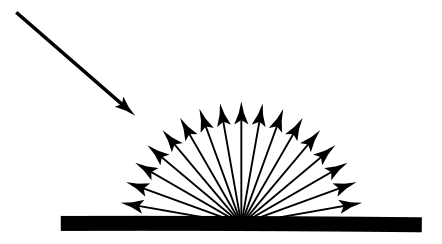
\includegraphics[scale=0.35]{media/Diffuse_Reflection.png}
	\caption{Diffuse reflection diagram. Source: Wikimedia Commons}
	\label{diff1}
\end{figure}

Our diffuse material follows Lambert's Cosine Law, this is the BRDF that our path tracer will use for this material. Lambertian objects has more probability for ray scattering when is close to the normal. The distribution is $cos(\phi)$ where $\phi$ is the angle from the normal. We can achieve this distribution by picking points on the surface of the unit sphere centred in (p + $\vec{N}$). The $pdf$ in our case is $\frac{cos(\phi)}{\pi}$.

\begin{figure}[!ht]
	\centering
	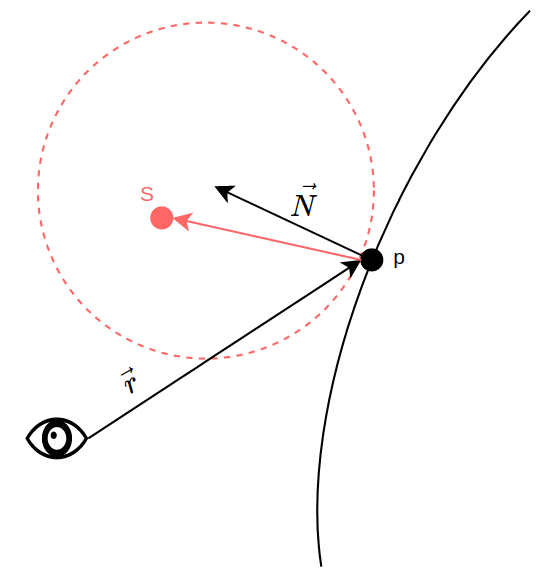
\includegraphics[scale=0.35]{media/random_ray.png}
	\caption{Random diffuse bounce ray}
	\label{diff2}
\end{figure}

The easiest way to get those points is by using a rejection method. In our case, we will pick a random point in the unit cube where all coordinates are in range -1 to +1 and then reject this point if is outside the sphere. If a point S of cartesian coordinates $x_0, y_0, z_0$ is inside a sphere of radius R then 

\begin{algorithm}[caption={random\_on\_unit\_sphere}]
input: 
output: $Vector_3$
begin
  $Vector_3$ s
  do
    s = (random[-1,1], random[-1,1], random[-1,1])
  while $||s||^2 \geq 1$
  return $\frac{s}{||s||}$
end
\end{algorithm}

Once we have a random point, the new scattered ray is the one that goes from the hit point to this.

\begin{figure}[H]
	\centering
	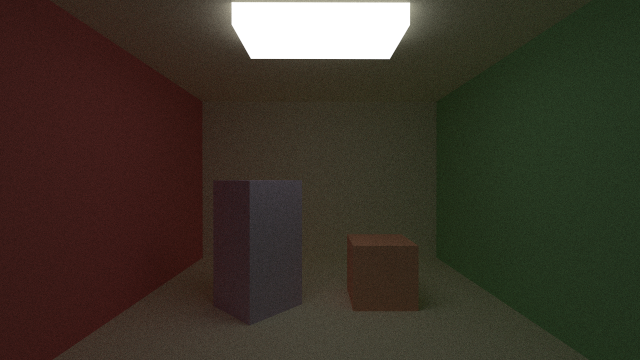
\includegraphics[scale=0.65]{media/cornell_normal_test.png}
	\caption{Diffuse objects example. Rendered with our application.}
	\label{diff3}
\end{figure}

\subsection{Metals}

In contrast to diffuse objects, metal objects do not scatter rays randomly. In this case, when a ray hits a metallic surface, this is scattered in one direction. According to the law of reflection: the angle of incident light, $\phi_i$, is the same as the angle of the reflected light, $\phi_r$. For simplicity, we just assumed a perfect reflection. So, our BRDF is a perfect reflection function using a parameter for roughness.

\begin{figure}[H]
	\centering
	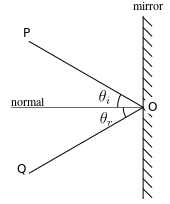
\includegraphics[scale=0.65]{media/Reflection_angles.png}
	\caption{Ray reflection diagram. Source: Reflection (physics), Wikipedia }
	\label{metal1}
\end{figure}

Given an incident direction $\vec{P}$, from camera or scattered from other object, and the surface normal $\vec{N}$, the reflected ray $\vec{Q}$ (all in unit vectors) is:

\begin{equation}
	\vec{Q} = \vec{P} + 2(\vec{P}\cdot\vec{N})\vec{N}
\end{equation}

Once we have the reflected point, the new scattered ray is the one that goes from the hit point to this.

Right now, we have mirror-like metals that perfectly reflect the incident rays. But as we know, not all metals are 100\% glossy, so we will add a roughness parameter to the material, a value in the range of 0 to 1. A metal object with roughness 0 will be smoothly polished. What this roughness parameter does is randomly disturbed the point for the reflected beam, keeping the direction.

\begin{figure}[H]
	\centering
	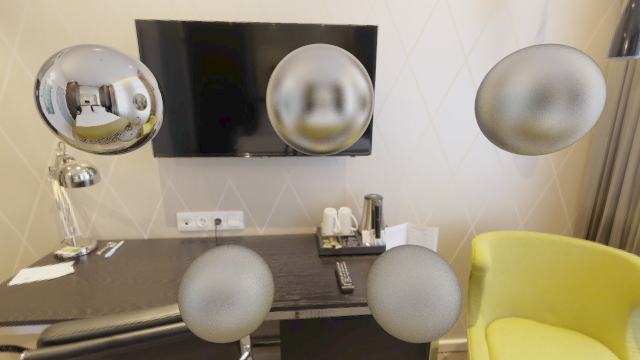
\includegraphics[scale=0.65]{media/example_metals.png}
	\caption{Example of metallic spheres with different roughness value. Rendered with our application.}
	\label{metal2}
\end{figure}

\subsection{Dielectrics}

Materials like glass, water or diamond are dielectric. That means they can reflect light and at the same time let the light pass through, this last is called refraction. For simplicity, we only will go to generate one scattered ray per iteration, that may be a reflection or refracted ray. Each material has her own refractive index that describes how light propagates through them and can be described by Snell's law of refraction. It's defined as $\eta = c/v$. Where $c$ is the speed of light in vacuum and $v$ is the speed of light in the material (or medium). Some common materials have this following refractive index.

\begin{itemize}

	\item Vacuum 1
	\item Air 1.000293
	\item Water 1.333
	\item Ice 1.31
	\item Flint glass 1.69
	\item Sapphire 1.77
	\item Diamond 2.42

\end{itemize}

\subsubsection{Snell's Law of Refraction}

\begin{figure}[H]
	\centering
	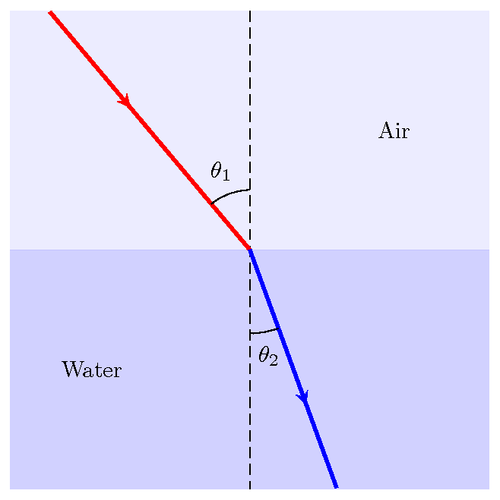
\includegraphics[scale=0.45]{media/refraction.png}
	\caption{Snell's law diagram.}
	\label{snell}
\end{figure}

Snell's law states that the ratio of the sines of the angles of incidence and refraction is equivalent to the ratio of the indices of refraction, via the cosines of the angle of incidence $\theta_1$ and angle of refraction $\theta_2$, we get:

\begin{equation}
	\frac{sin(\theta_2)}{sin(\theta_1)} = \frac{\eta_1}{\eta_2}
\end{equation}

We can rewrite this as follows:

\begin{equation}
	sin(\theta_2) = \frac{\eta_1}{\eta_2} sin(\theta_1)\label{snlaw1}
\end{equation}

Given a normalized incident vector $\vec{v}$ (pointing from virtual camera or scattered from another surface toward the surface) and a normalized normal vector $\vec{n}$

\begin{equation}
	cos(\theta_1) = \vec{v} \cdot \vec{n}
\end{equation}

In order to get the refracted ray, we need to solve $sin(\theta_2)$ and $cos(\theta_2)$. From the fundamental trigonometric identity, we know that $sin^2(\theta_1) = 1 - cos^2(\theta_1)$, so $sin(\theta_1) = \sqrt[]{1 - cos^2(\theta_1)}$. Now, applying the Snell's law [\ref{snlaw1}], we get:

\begin{equation}
\begin{split}
	sin(\theta_2) & = \frac{\eta_1}{\eta_2} \sqrt[]{1-cos^2(\theta_1)}
\end{split}
\end{equation}

\begin{equation} \label{eq1}
\begin{split}
cos^2(\theta_2) & = 1 - sin^2(\theta_2) \\
 & = 1 - \left(\frac{\eta_1}{\eta_2} \sqrt[]{1-cos^2(\theta_1)} \right)^2 \\
 & = 1 - \left(\frac{\eta_1}{\eta_2} \right)^2 \left(1-cos^2(\theta_1)\right) \\
cos(\theta_2) & = \sqrt[]{1 - \left(\frac{\eta_1}{\eta_2} \right)^2 \left(1-cos^2(\theta_1)\right)} \\
cos(\theta_2) & = \sqrt[]{1 - \left(\frac{\eta_1}{\eta_2} \right)^2 \left(1 - ( \vec{v} \cdot \vec{n})^2\right)}
\end{split}
\end{equation}

\begin{figure}[H]
	\centering
	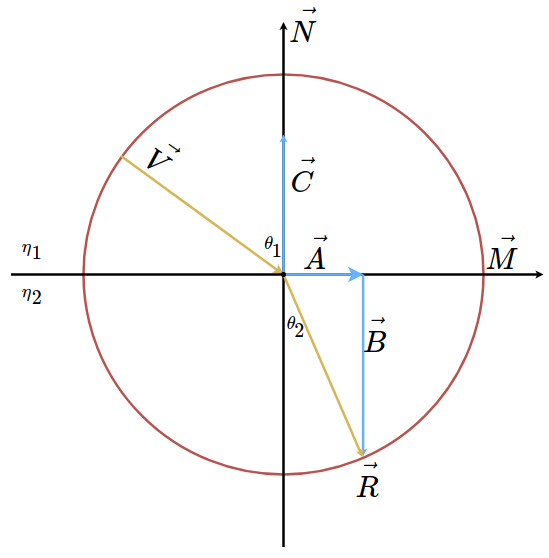
\includegraphics[scale=0.45]{media/refraction_unit_sphere.png}
	\caption{Refracted ray calculation.}
	\label{snell2}
\end{figure}

We can define the refracted ray $\vec{R}$ as $\vec{R} = \vec{A} + \vec{B}$, where $\vec{A} = \vec{M} sin(\theta_2)$, $\vec{B} = -\vec{n} cos(\theta_2)$, $\vec{M} = \frac{\vec{v}+\vec{C}}{sin(\theta_1)}$ and $\vec{C} = cos(\theta_1)\vec{n}$. With all this vectors we can reconstruct the formula for the refracted ray as follows:

\begin{equation} \label{refracted_ray}
\begin{split}
\vec{R} & = \vec{A} + \vec{B} \\
 & = sin(\theta_2) \frac{\left(\vec{v} + cos(\theta_1)\vec{n}\right)}{sin(\theta_1)} - \vec{n} cos(\theta_2) \\
 & = \frac{sin(\theta_2)}{sin(\theta_1)} \left(\vec{v} + cos(\theta_1)\vec{n}\right) - \vec{n} cos(\theta_2) \\
 & = \frac{\eta_1}{\eta_2} \left(\vec{v} + cos(\theta_1)\vec{n}\right) - \vec{n} cos(\theta_2) \\
\vec{R} & = \frac{\eta_1}{\eta_2} \vec{v} + \left(\frac{\eta_1}{\eta_2} cos(\theta_1) - cos(\theta_2) \right) \vec{n} \\
\vec{R} & = \frac{\eta_1}{\eta_2} \vec{v} + \left(\frac{\eta_1}{\eta_2} (\vec{v} \cdot \vec{n}) - cos(\theta_2) \right) \vec{n} \\
\end{split}
\end{equation}

Replacing $cos(\theta_2)$ by the equation \ref{eq1}, we get the equation to calculate the refracted ray:

\begin{equation} \label{refracted_ray_2}
\begin{split}
\vec{R} & = \frac{\eta_1}{\eta_2} \vec{v} + \left(\frac{\eta_1}{\eta_2} (\vec{v} \cdot \vec{n}) - \sqrt[]{1 - \left(\frac{\eta_1}{\eta_2} \right)^2 \left(1 - ( \vec{v} \cdot \vec{n})^2\right)} \right) \vec{n} \\
\end{split}
\end{equation}

Also, $cos(\theta_2)$ is the discriminant of the equation. When $cos(\theta_2) < 0$ that means that we have \textbf{total internal reflection}. That occurs, in some cases, when the light travels from a medium with a higher refractive index to one with a lower and the sines of the angle of refraction needs to be greater than one. For example, in our application, it can occur when a lightning bolt that has passed through a dielectric object comes out of it into a vacuum.

\subsubsection{Fresnel Equations}

When light hits the interface between two mediums with different refractive index, both reflection and refraction may occur. The Fresnel equations describe the ratios of the reflection and transmission of light. This reflection varies with the angle of incidence. In computer graphics, is very common to use Schlick's Approximation \citep{Schlick1994} to approximate the value of Fresnel Equations because is less expensive. That's the reason why we use this formula of 5th grade to approximate the Fresnel value.

\begin{equation} \label{schlick}
\begin{split}
R(0) & = R_0 + (1 - R_0) \left(1 - cos(\theta)\right)^5 \\
R_0 & = \left(\frac{\eta_1 - \eta_2}{\eta_1 + \eta_2}\right)^2
\end{split}
\end{equation}

\begin{figure}[H]
	\centering
	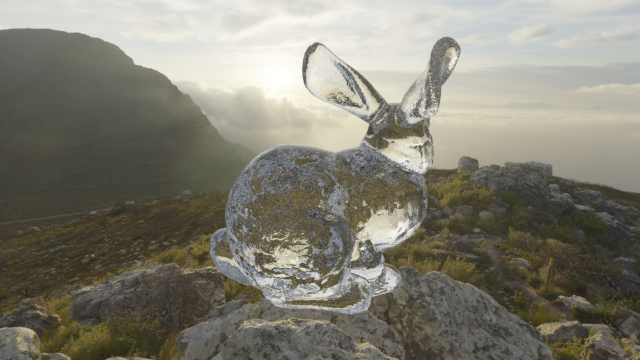
\includegraphics[scale=0.65]{media/CapeHill_cristal_bunny.png}
	\caption{Glass bunny, $\eta_1 = 1.42$. Rendered with our application.}
	\label{dielectric1}
\end{figure}

\subsection{Diffuse light}

These objects emit light and absorb the rays that reach them. For example, a primary ray that leaves the camera bounces off a diffuse or specular surface and hits a light source is totally absorbed and the path is cut off at that point.

\subsection{Textures}

We can use images to define the material of an object in the scene, these images are known as textures. The textures allow us to add more detail to our objects than using, for example, a triangle colouring. Texture mapping is the method in which we must map a 2D image to a 3D model.

There are different types of textures. We have for example the colour map (diffuse), gloss map, opacity map for transparency, displacement map to generate 3D effects, etc. For simplicity, for this project, we will only use colour maps.

A 3D model can contain more than one texture, thus increasing the quality of the detail of the model. This is known as multitexture. But due to lack of time, in this project, we decided to implement only one texture per 3D model.

As we explained in the section on the ray-triangle intersection algorithm, this algorithm already provides us with the UV coordinates that allow us to perform texture mapping. To be able to make this mapping, the triangle mesh must have defined for each of its polygons the texture coordinates.

In the Möller-Trumbore algorithm, we explained that the calculated UV coordinates correspond to the barycentric coordinates. So we can use them to interpolate the texture coordinates. We have to go from \textit{triangle space} to \textit{texture space}. For this, we must use the equation \ref{barycentric} where $V_0$, $V_1$ and $V_2$ are in this context the texture coordinates $T_0(U_0, V_0)$, $T_1(U_1, V_1)$ and $T_2(U_2, V_2)$ from the triangle.

\begin{figure}[H]
	\centering
	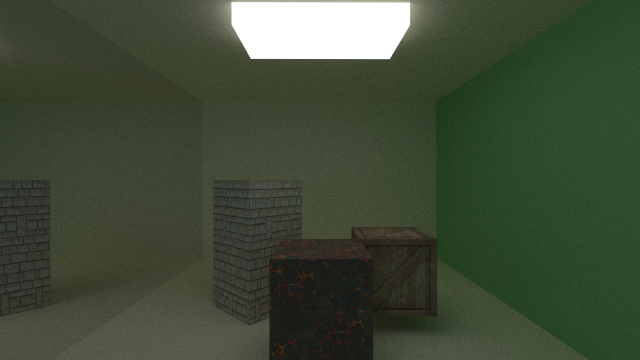
\includegraphics[scale=0.65]{media/cornell_textures.png}
	\caption{Scene with objects using textures. Rendered with our application.}
	\label{textures_1}
\end{figure}

\subsection{Skybox}

In scenes where you are not inside a room, such as the Cornell Box, you can use for the background some flat colour or sort of gradient. But this is quite limited and not very fancy, so is usually to use skyboxes that allow us to add a background to our scene, making it richer in detail. It is a generally used resource in video game design because they allow us to create levels that look bigger than they are. It also allows us to integrate elements in the scene without having to add unnecessary geometry because we are using only a 2D texture. They are often used to represent skies and elements that are far away from the epicentre of the scene. It is for this reason that skyboxes remain static, to create the illusion of distance. In the Figure \ref{skybox1} we can see a very clear example, for the buildings in the background instead of modelling them they are in a texture just like the sky.

\begin{figure}[H]
	\centering
	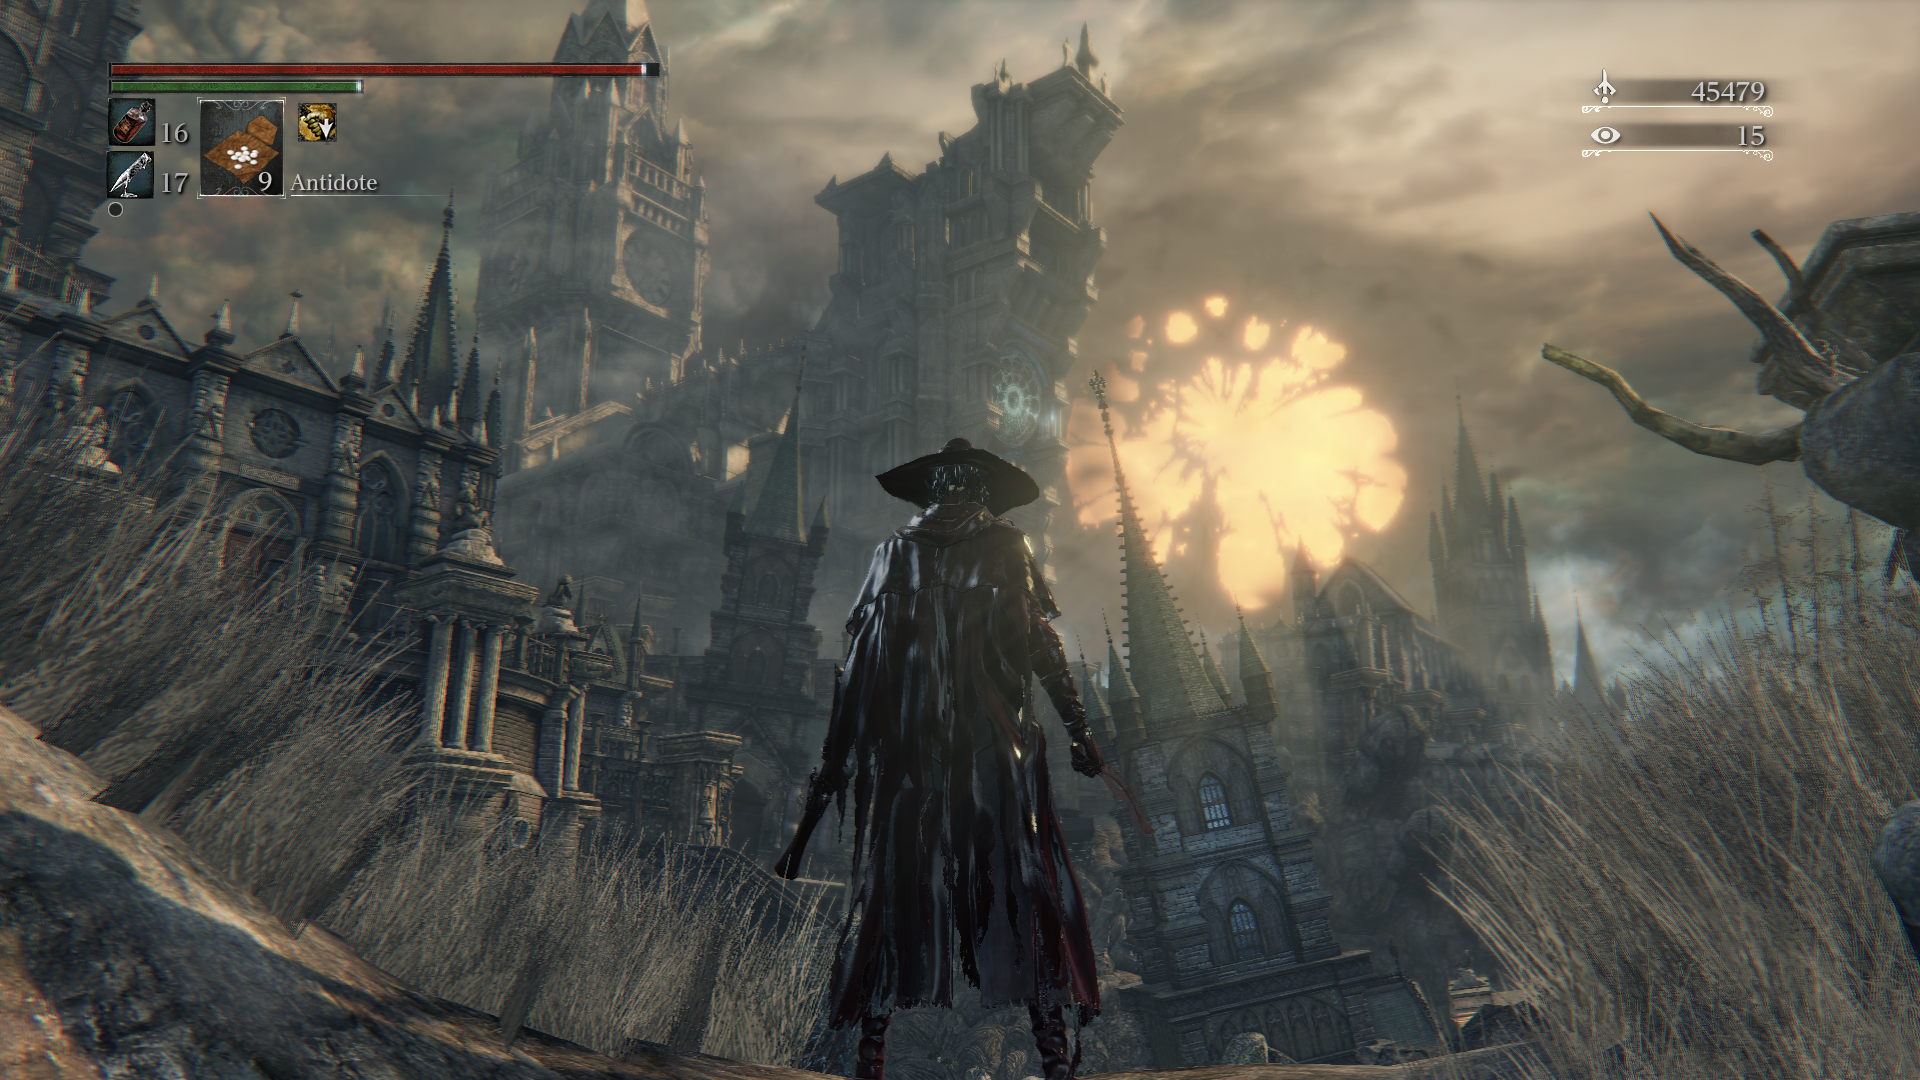
\includegraphics[scale=0.20]{media/skybox.png}
	\caption{Image extracted from Bloodborne game.}
	\label{skybox1}
\end{figure}

When we're using a skybox, what we're doing is encapsulating the whole scene in a cuboid. This cuboid is where we will map the texture that the skybox will represent using the cube mapping technique. Usually, a cube map texture is defined as shown in Figure \ref{skybox2}

\begin{figure}[H]
	\centering
	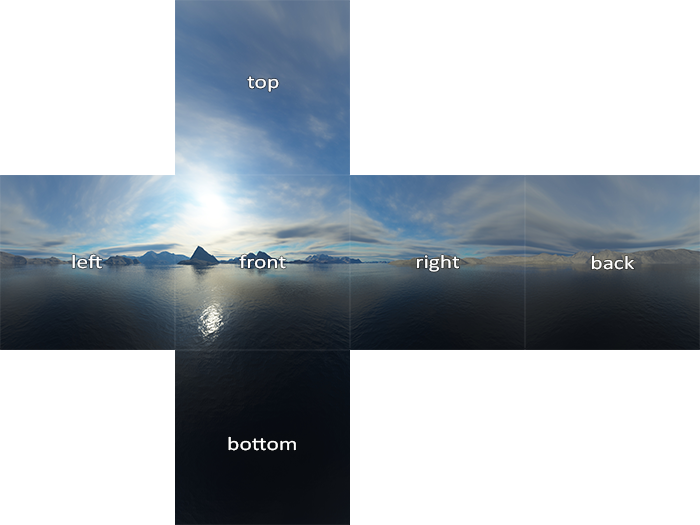
\includegraphics[scale=0.45]{media/cubemaps_skybox.png}
	\caption{Cube map texture.}
	\label{skybox2}
\end{figure}

In our case, we have decided to use six textures (six faces of the cuboid) and map it on each of the corresponding faces of the defined cuboid that wraps the scene. We can see an example of a scene using a skybox in Figures \ref{metal2} and \ref{dielectric1}.

\section{Acceleration Data Structures}

In graphic applications where Ray Tracing or Path Tracing is implemented, the use of acceleration structures is very common. An acceleration structure is a data structure that, as the name suggests, allows us to consult the information in a faster and optimal way. In Path Tracing, as we have been seeing, billions of rays can be launched along with the rendering and a scene can have millions of primitives, so not making use of this type of data structure greatly affects the performance of the application. As we will see later on, we have for each version (sequential and parallel) two sub-models in which we use an accelerator data structure and another one in which we simply consult the whole list of primitives to determine the nearest in collision detection. We will see the improvement that these structures offer us and why they are very important and used.

We have different types of data structures that allow us to improve the performance of our algorithm. The most common data structures used are: \textit{regular grid} proposed by \citep[pp.~12--26]{Fujimoto1986}, K-d Tree invented by \citep[p.~509--517]{Bentley1975}, Octrees, variation from K-d Tree, proposed by \citep{DonaldMeagher1982} for 3D computer graphics applications Bounding Volume Hierarchy (BVH) \citep{Gunther2007}. For this project we decided to use the Bounding Volume Hierarchy because of their low memory usage and flexibility in adapting to scene geometry.

\subsection{Bounding Volume Hierarchy}

A Bounding Volume Hierarchy is a tree-type data structure in which each node represents the bounding box of primitives. These primitives are \textit{stored} in the leaf nodes. Each intermediate node carries the bounding box of its children until it reaches the root node of the tree where it represents the bounding box of the whole scene. This data structure allows us to test ray-triangle collisions quickly and efficiently. If we launch a ray, and when querying the root node we do not have a collision, then we would continue launching new rays from the camera through the scene. However, in this case, if we do not have an accelerating structure we would need to test all the primitives in our scene to conclude that finally there has been no collision, and this is very inefficient.

\begin{figure}[H]
	\centering
	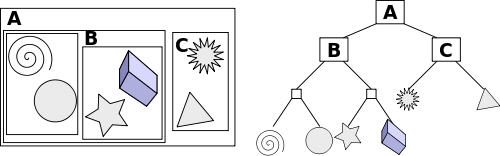
\includegraphics[scale=0.65]{media/BVH_example.png}
	\caption{Bounding Volume Hierarchy example. Source: Wikipedia. Bounding volume hierarchy.}
	\label{bvh1}
\end{figure}

\subsubsection{BVH Construction}

There are many ways to build the BVH and the way we do it can affect to a greater or lesser extent the performance of it since it is a structure that we must go through millions of times and the way it has been built will make us go through the tree more or fewer times.

The simplest way to build our tree is to do it while reading the primitives of the scene.  This is a very naive solution because we can be putting two primitives with the same father node, and they can be very far away from each other. This can eventually affect performance, as we will need to go through the tree more exhaustively. Even so, it's quite a better solution than going through a list. For this reason, we must find a more reasonable way to build this tree that allows us to go through it as few as possible.

\citep[p.~375--384]{Lauterbach2009} were the first to present a parallel method of building BVHs by ordering the primitives in the scene along a space-filling curve. The main idea proposed by \citep[p.~375--384]{Lauterbach2009} is to assign a \textit{Morton code} (space-filling curve) to each of the primitives and then order them. Once sorted, we build the tree where each intermediate node corresponds to a range within all the generated Morton codes being the root the range between $[0, n-1]$.

This \textit{Morton code}, presented by \citep{Morton1966ACO}, maps n-dimensional data to one dimension preserving its locality. The $z$-value of a point is calculated by interleaving the binary values of its coordinates. For example, if we have a three-dimensional point $(x,y,z)$, its z-value will be $x_0y_0z_0x_1y_1z_1...$ where the $x$ coordinate is represented by its binary representation $0bx_0x_1x_2...$, the same for $y$ and $z$ coordinate.

Once we have assigned a Morton code to each of the primitives, we order them according to this one and proceed to build the tree. The tree that we will build will be a binary radix tree. This kind of tree is characterized by having in its nodes the representation of the keys and in each intermediate node we have the longest shared common prefix. In Figure \ref{radix} we can see an example of a binary radix tree.

\begin{figure}[H]
	\centering
	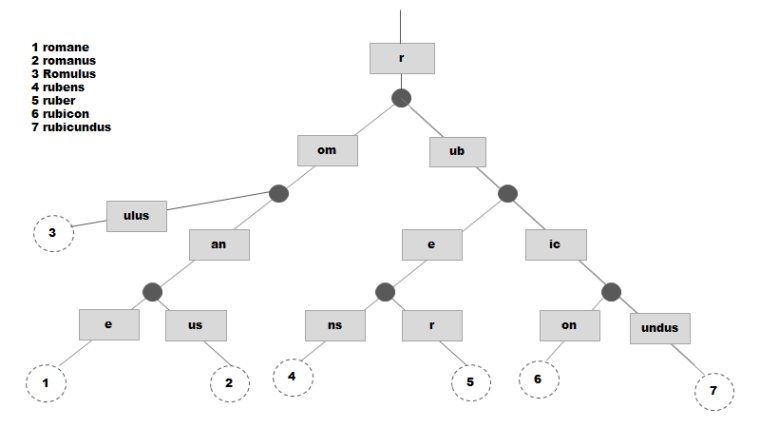
\includegraphics[scale=0.45]{media/radixtree.png}
	\caption{Example of binary radix tree. Source: Wikipedia. Radix tree.}
	\label{radix}
\end{figure}

For each internal node, we must find the range $[i,j]$ that it represents and once we have determined the range, we can obtain the split position, denoted by $\gamma in [i,j]$. The split position tells us that the Morton codes are equal up to the $\gamma$ bit, where $k_{\gamma} = 0$ and $M_{\gamma +1} = 1$. So the subtrees will have range $[i, \gamma]$, $[\gamma+1,j]$.

\begin{figure}[H]
	\centering
	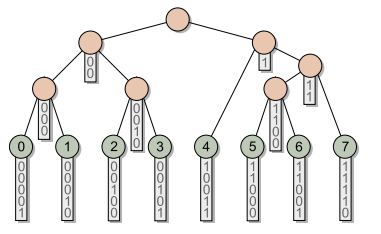
\includegraphics[scale=0.45]{media/radix_tero_1.png}
	\caption{Ordered radix tree. Source: \citep{Karras2012}.}
	\label{radix_tero}
\end{figure}

As we have already indicated, we must first find the range [i,j] in which the internal node Ii covers. To do this we will define i as one of the limits of this range. First of all we must determine the direction $d$ (that can be 1 or -1) we should go, for it, we will take the code $k_i$, and we will compare the length of the longest common prefix, denoted by $\delta(i,j)$, with its two surroundings $k_{i-1}$ and $k_{i+1}$. Since we know that each internal node has exactly two children, we know that $k_i$ and $K_{i+d}$ belongs to the internal node $I_i$. 

We know that all codes belonging to $I_i$ share a common prefix that differs by one bit from its brother, by definition. Therefore, this implies that the length of the lower boundary is given by $\delta_{min} = \delta(i,i-d)$, so $\delta(i,j) > d_{min}$ for all $k_j$ belonging to $I_i$. We can satisfy this condition by comparing $\delta(i,i+1)$ with $\delta(i,i-1))$ and choosing $d$ as the largest one.

The other boundary can be found by searching for the largest $l$ that satisfy $\delta(i,i+ld) > \delta_{min}$. We can define an upper bound power of 2 and increasing the value until it no longer satisfy the inequality. Once we have this upper bound, we perform a binary search to find $l$ in the range $[0, l_{max}-1]$. The idea is set to one each bit of $l$ unless the new value would fail to satisfy the inequality $\delta(i, i + (l + t)d) > \delta_{min}$. Once we finish, the search the other bound is given by $j = i + ld$. If $j < i$, we need to swap the values. We can see the implementation below, where the function $lcp$ represents $\delta(i,j)$.

\begin{algorithm}[caption={range}, label={range_alg}]
input: int i
output: $int_2$
begin
  $d = sgn(\delta(i, i+1) - \delta(i, i-1))$
  $\delta_{min} = \delta(i, i-d)$
  
  $l_{max} = 2$  
  while $\delta(i, i+ld) > \delta_{min}$
    $l_{max} = 2l_{max}$

  $l = 0$
  while $t = [1, ... , \lceil \frac{l_{max}}{4} \rceil, \lceil \frac{l_{max}}{2}] \rceil$
    if $\delta(i, i + (l+t)d) > \delta_{min}$
      $l += t$
  
  $j = i + ld$
   
  return $(i,j)$
end
\end{algorithm}

Once we have obtained the range in which an internal node covers, we must find which split position $\gamma$ to choose. To do this, we will choose the largest bit that differs between two Morton codes within the given range. The most efficient way to perform this search is by performing a binary search, starting with the Morton code corresponding to the lower limit of the range, $k_i$, and moving forward by decreasing it exponentially. At each step, we will look to see if the new proposed position satisfies $\delta(i,\gamma) > \delta(i,j)$. If the new position satisfies the condition, we continue to move forward until we can no longer advance in the search. The function $_clz$ count the number of leading zero bits in a 32-bit integer. We can use it to find the split position of two Morton codes.

\begin{algorithm}[caption={split}, label={split_alg}]
input: int i, int j
output: $int$
begin
  if $i == j$
    return -1

  $prefix = \_clz(k_i \XOR k_j)$  
  $split = i$
  $step = j - i$
  do
    $step = \frac{step + 1}{2}$
    $newSplit = split + step$
    
    if $newSplit < j$
      $splitPrefix = \_clz(k_i \XOR k_{newSplit})$
      if $splitPrefix > prefix$
        $split = newSplit$
  while step $>$ 1
  return $split$
end
\end{algorithm}

Once we have obtained the split position and the range covered by the internal node, we can build the internal node $I_i$ by following these two rules:

\begin{enumerate}\label{child_assing}

\item If $\gamma = i$, then the left child of the internal node $I_i$ belongs to a leaf node, therefore to a primitive otherwise, it belongs to the internal node $I_{\gamma}$.

\item If $\gamma + 1 = j$, then the right child of the internal node $I_i$ belongs to a leaf node, therefore to a primitive otherwise, it belongs to the internal node $I_{\gamma+1}$.

\end{enumerate}

\subsubsection{Sequential CPU - BVH construction implementation}

The construction of the BVH in the sequential version is as simple as going through the set of intermediate nodes, $I$, and for each of them calculate the range it occupies and the separation point using the algorithms defined previously, \ref{range_alg} and \ref{split_alg}. Once we have the splitting point, we can assign the left and right child as defined in \ref{child_assing}. $L$ is the set of leaf nodes.

\begin{algorithm}[caption={BVH construction CPU - sequential}, label={cpu_seq_bvh}]
input: $I$, $L$
output: Node
begin
  foreach $idx \in [0, |I|-1]$
    $(i,j) = range(idx)$
    $\gamma = split(i,j)$
    
    if $ \gamma == i $
      $I_{idx} \leftarrow left = L_{\gamma}$
    else 
      $I_{idx} \leftarrow left = I_{\gamma}$
    
    if $ \gamma+1 == j $
      $I_{idx} \leftarrow left = L_{\gamma+1}$
    else 
      $I_{idx} \leftarrow left = I_{\gamma+1}$
  end
  return $I_{0}$
end
\end{algorithm}

Finally, once the tree is built, we only have to assign to each internal node the bounding box. The strategy varies according to the architecture on which we have programmed the application.

\subsubsection{Parallel CPU (OpenMP) - BVH construction implementation}

For the OpenMP version, the concept is the same. In OpenMP, we have the pragma omp\\
(\lstinline|#pragma omp <directives>|) with a series of directives. This pragma is nothing more than a directive that tells the compiler to use pragmatic rules. The directive that we should use in this case is the \textbf{for} directive that allows us to split the number of iterations among the threads. We'll use the \textbf{schedule} clause that determines which loop iteration each thread executes. For our case we've decided to use a static schedule, meaning that before the loop iterations are executed they're already distributed to the threads, with a chunk size of 8. Each thread gets 8 consecutive iterations. The assignment of iterations to the threads is done through the Round-Robin algorithm. In \ref{cpu_par_bvh} we can see the pseudo-code of this version.

\begin{algorithm}[caption={BVH construction CPU - parallel}, label={cpu_par_bvh}]
input: $I$, $L$
output: Node
begin
  #pragma omp for schedule(static, 8)
  foreach $idx \in [0, |I|-1]$
    $(i,j) = range(idx)$
    $\gamma = split(i,j)$
    
    if $ \gamma == i $
      $I_{idx} \leftarrow left = L_{\gamma}$
    else 
      $I_{idx} \leftarrow left = I_{\gamma}$
    
    if $ \gamma+1 == j $
      $I_{idx} \leftarrow left = L_{\gamma+1}$
    else 
      $I_{idx} \leftarrow left = I_{\gamma+1}$
  end
  return $I_{0}$
end
\end{algorithm}

The reason for using a static schedule is the reason of the low overhead. It also has a better location than dynamic or guided but in our case as each node is independent it doesn't affect us.

\subsubsection{Parallel GPU (CUDA) - BVH construction implementation}

On \texttt{CUDA}-compatible (NVIDIA) graphics cards we have a series of spindles called \textit{Multiprocessor Streaming} (SM). These, in turn, are composed of the \textit{Streaming Processors} that are responsible for executing the instructions.

At CUDA we have the concepts of kernels. A kernel in the \texttt{CUDA} environment refers to a function executed by the GPU in N threads. Kernels are defined with the \lstinline|__global__| specifier. There are other specifiers such as \lstinline|__host__| and \lstinline|__device__| that indicate which device can run it. These kernels are organized into a hierarchy grouped by blocks and can be distributed in a grid. All threads within a block are executed concurrently and when they are finished, the unit in charge of their distribution launches new blocks. Also, within a block, threads are distributed in groups of 32 forming warps. When a warp is executed, 32 threads execute the same instruction at the same time at the hardware scale.

The syntax for calling a CUDA kernel varies from a traditional C or C++ function. To call a CUDA kernel we must first configure it properly, for this we have the following syntax \lstinline|<<<GS, BS, SM, S>>>|, e.g., \lstinline|cuda_kernel<<1.1>>|. The first two parameters are mandatory.

\begin{itemize}

\item \textbf{GS}: Specifies the size of grid. Three-dimensional value (x,y,z). We can work with 1D, 2D and 3D arrays. In our context, we only will work with 1D array.
\item \textbf{BS}: Specifies the size of block. Three-dimensional value (x,y,z). We can work with 1D, 2D and 3D arrays. In our context, we only will work with 1D array.
\item \textbf{SM}: Specifies the number of bytes in shared memory. When a kernel have shared memory, this needs to be dynamically allocated per block for this launch.
\item \textbf{S}: Specifies the associated stream.

\end{itemize}

When we have an input set, in this case, the uninitialized intermediate nodes, and an output set, the initialized intermediate nodes, and both have the same size a common approach is to get a single thread responsible for one of the data in the set. On current GPUs, the maximum number of threads per block is 1024. If we decide to use $n$ threads per kernel launch, the block size in our case will be $n$. So, if the input array has size of $m$, we need at least $\frac{m}{n}$ blocks. The problem we may have here is when $m$ is not divisible by $n$, so we will throw more blocks than we need to cover all the space. Therefore, the distribution of the grid ($GS$) and the blocks ($BS$) will be as follows

$$
BS = n
$$
$$
GS = \frac{m + n - 1}{n}
$$

In the kernel to be able to index which position of our array is calculating each vector we can index it as we see in the Figure \ref{indexing}.

\begin{figure}[H]
	\centering
	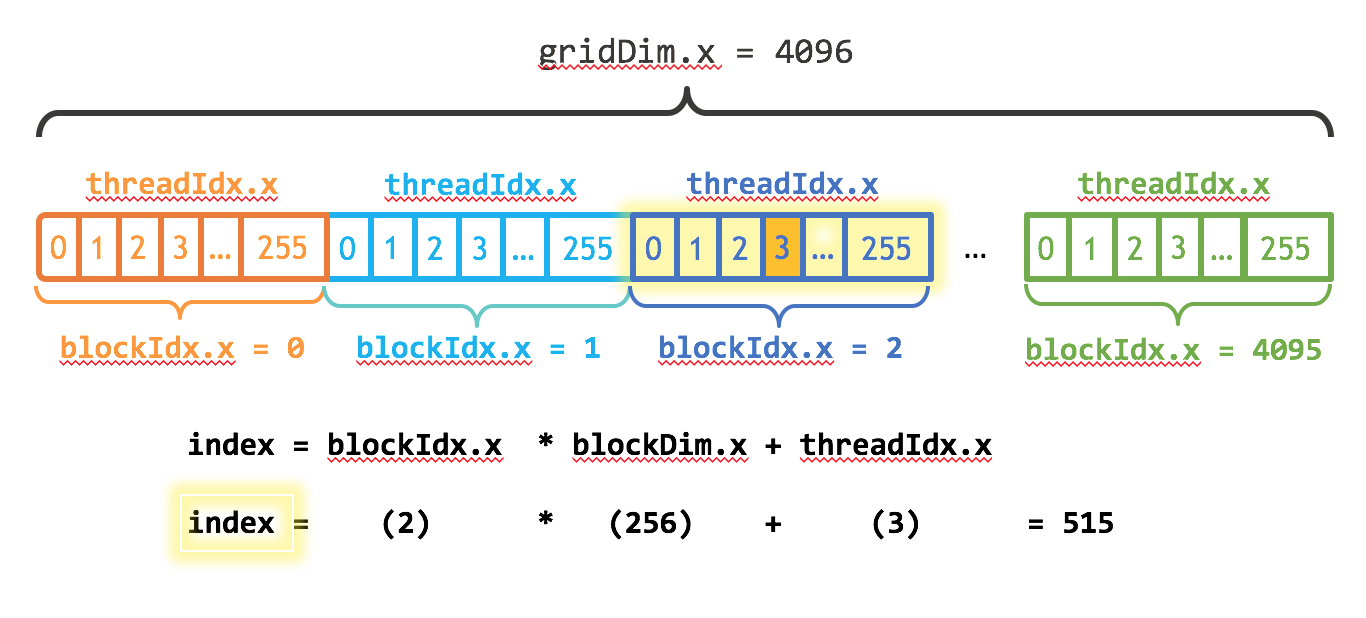
\includegraphics[scale=0.45]{media/cuda_indexing.png}
	\caption{CUDA indexing example. Source: \textit{NVIDIA}}
	\label{indexing}
\end{figure}

So the algorithm would look like this

\begin{algorithm}[caption={BVH construction GPU - parallel}, label={gpu_par_bvh}]
input: $I$, $L$, $\#OBJS$
output:
begin
  $idx = blockIdx.x * blockDim.x + threadIdx.$ 
  if $idx < \#OBJS$
    $(i,j) = range(idx)$
    $\gamma = split(i,j)$
    
    if $ \gamma == i $
      $I_{idx} \leftarrow left = L_{\gamma}$
    else 
      $I_{idx} \leftarrow left = I_{\gamma}$
    
    if $ \gamma+1 == j $
      $I_{idx} \leftarrow left = L_{\gamma+1}$
    else 
      $I_{idx} \leftarrow left = I_{\gamma+1}$
end
\end{algorithm}

\subsubsection{Bounding-box calculation CPU}

For the CPU version, we go through the tree in post-order to calculate the bounding boxes of each internal node. 

\subsubsection{Bounding-box calculation GPU}

For the GPU version, we take advantage of the parallel calculation of all the bounding boxes. To do this, we assign a leaf node to each thread. We'll need to use an atomic counter to mark those nodes we've already visited. So that two threads don't access the same node at the same time and cause a memory error. For each internal node $I_j$, the first thread that accesses it will be in charge of calculating the bounding box by joining the AABB of the children of the internal node $I_j$.

\section{Scene manager}

To avoid having to hard-code the scenes in the application's code, we decided to create a class, Scene.hh, that would handle the scene. This class is in charge of reading a text file with a specific format in which the scene we want to render is defined. In this input file, we can specify different entities of the scene: the camera, the 3D models and the skybox. For the 3D models, we can define a material from the ones explained above or if we want a texture. Also, we can specify a series of geometric transformations to be able to manipulate it.

As we discussed a section further back, we decided to use triangles because in this way we could render 3D models that were defined by meshes of triangles. This allowed us to describe more complex scenes and study the performance of our application in more profundity. To be able to read these triangle patterns, a very simple parser has been developed that allows us to load .obj files into the application, one of the standards in terms of 3D model definition. In a .obj file, we have different elements that we must know how to recognize.

\subsubsection{Geometric vertices}

\textbf{v x y z}

This describes a geometric vertex. The parameters $x$, $y$, $z$ represents their coordinates. Sometimes, another parameter $w$ can appear to define the weight. That can happen when specifies rational curves and surfaces. The coordinates $(x,y,z)$ are floating-point numbers that define the position of the vertex in three dimensions.

\subsubsection{Texture vertices}

\textbf{vt u v w}

This is the texture coordinates. When we create a 3D model with a tool like Blender, Maya, etc. it gives us the option to generate the texture coordinates for our model. If we don't do this step, or we don't use a 3D model that has the texture coordinates mapped, then we won't be able to apply a texture to it, because we won't know how to map it. The components $v$ and $w$ are optional because we can use 1D texture, but it is more common to use 2D textures. Also, we can have a 3D texture that requires all three coordinate. The three components $(u, v, w)$ are floating-point numbers.

\subsubsection{Vertex normal}

\textbf{vn i j k}

This describes the normal with components $(i,j,k)$. For polygons, vertex normals are used in place of the actual facet normals. The components $(i,j,k)$ are floating-point numbers.

\subsubsection{Polygon Faces}

\textbf{f v/vt/vn v/vt/vn v/vt/vn v/vt/vn...}

This is the face. The format, in this case, is quite different. Here we are indicating all the vertices that compose a face that can be formed by more than one vertex. The simplest example can be a plane, which is formed by four triangles that make up a face. To be able to interpret this in triangles, we have to do a fan triangulation. We will choose one vertex and from them, we will generate triangles using the other vertices reading in groups of three.

\section{Image Filters}

In this section, we will talk about image filters. As we have commented on several occasions, the most important problem of our Monte Carlo Path Tracing is the noisy images that it generates. We should make infinite bounces to calculate the final colour of a pixel. This is not possible due to the limited computational resources and rendering time. That is the reason why we have to limit the depth of the paths of light traced by using a cut-off.

 The noise it generates is known as salt-and-pepper noise. In the introduction of this chapter, we have talked about how to reduce the image noise by increasing the number of samples we use per pixel. It is easy to see that increasing the number of samples taken per pixel increases the image render time since more calculations have to be done for each given pixel. Due to this, we have considered that an effective way to reduce the noise of the image, without increasing considerably the number of samples per pixel, is to use denoising image filters.

The filters that we have selected are Mean Filter, Median Filter and Bilateral Filter. For each rendered image we will apply the filters and at the end, we will determine which one works better for our scenarios.

\subsection{Mean Filter}

The mean filter is one of the simplest spatial filters we have. It consists of creating an $n \times n$ sliding-window centred on a pixel $(i,j)$ that moves around the image and replaces the pixel value $(i,j)$ with the window average. This window, also known as kernel, can have any kind of shape but usually, a square is used. The smoothing effect depends on the size of the kernel. The bigger it is, the more smoothing. Usually a $3 \times 3$ kernel filter size is used, an example of this is shown in Figure \ref{mean_filter}, but as we have said this kernel can be larger\footnote{A kernel filter where $n < 3$ would not be useful, since we would be going through all the pixels of image calculating the average with itself.} as needed.

\begin{figure}[H]
	\centering
	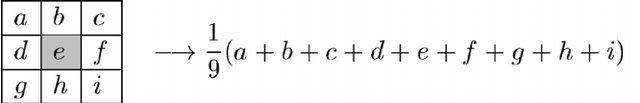
\includegraphics[scale=0.45]{media/mean_filter.jpg}
	\caption{Filtering approach of mean filter with $3 \times 3$ sliding-window: \citep{Lyra2011}.}
	\label{mean_filter}
\end{figure}


\subsection{Median Filter}

The median filter follows the same concept as the one mentioned above. We define a slider window $n \times n$ centred on the pixel $(i,j)$, but in this algorithm instead of calculating the average of all the pixels that are part of the kernel, we sort the values and select the median. In Figure \ref{median_filter} we can see an example with a $3 \times 3$ window.

\begin{figure}[H]
	\centering
	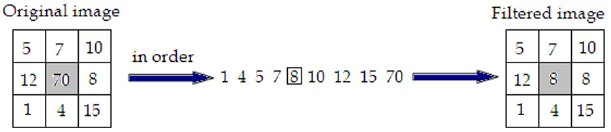
\includegraphics[scale=0.45]{media/median_filter.jpg}
	\caption{Filtering approach of median filter with $3 \times 3$ sliding-window: \citep{Lyra2011}.}
	\label{median_filter}
\end{figure}

\subsection{Bilateral Filter}

The bilateral filter is widely used in computer vision and image processing for edge-preserving smoothing. It is a non-linear filter for denoising and edge smoothing \citep[pp.~538--545]{Aurich1995}, \citep[pp.~839--846]{Tomasi1998} and \citep[pp.~1--73]{Paris2009}. In the field of image processing, edge smoothing is a technique that attempts to smooth noise while preserving the edges of objects. The bilateral filter replaces the intensity of each pixel with the weighted average of the surrounding pixels. These nearby pixels are defined through a window. This weight can be defined by a Gaussian function. The main purpose of the weighted function is to determine how closely are two points. The Gaussian functions arise from composing the exponential function with a quadratic concave function and are as follows.

\begin{equation}\label{gaussian_function}
f(x') = a e^{-\frac{(x'-b)^2}{2c^2}}
\end{equation}

We can define the bilateral filter as

\begin{equation}
I_{denoised}(x) = \eta^{-1} \sum_{y \in \Omega} G_{\sigma_s}(||y - x||) G_{\sigma_r}(|I(y) - I(x)|)I(y)
\end{equation}

and $\eta$ is defined ad

\begin{equation}
\eta = \sum_{y \in \Omega} g_s(||y - x||) g_r(|I(y) - I(x)|)
\end{equation}

where

\begin{itemize}
\item $I_{denoised}$ is the output image.
\item $I$ is the input image.
\item $x$ are the coordinates of the current pixel $(i,j)$ to be filtered.
\item $\Omega$ is the window centred in $x$.
\item $y$ are the coordinates from another pixel $(i', j')$ in windows $\Omega$.
\item $G_{\sigma_s}$ is the spatial kernel for smoothing differences in coordinates (pixel coordinate).
\item $G{\sigma_r}$ is the range kernel for smoothing differences in intensities (pixel colour).

\end{itemize}

For the range kernel and the space kernel we will use Gaussian functions. Following the definition of Gaussian function defined in \ref{gaussian_function} where $a = 1$, $(x' - b) = ||x - y||$ (Euclidean distance) and $c = \sigma^2$, then we have

\begin{equation}
G_{\sigma_s} = e^{- \frac{||y - x||}{2 \sigma_{s}^{2}}}
\end{equation}

and for $G_{\sigma_r}$ where $a = I(y)$, then we have

\begin{equation}
G_{\sigma_r} = e^{- \frac{|I(y) - I(x)|}{2 \sigma_{r}^{2}}} I(y)
\end{equation}

Finally we get

\begin{equation}
I_{denoised}(x) = \frac{\sum_{y \in \Omega} e^{- \frac{||y - x||}{2 \sigma_{s}^{2}}} e^{- \frac{|I(y) - I(x)|}{2 \sigma_{r}^{2}}} I(y)}{\sum_{y \in \Omega}e^{- \frac{||y - x||}{2 \sigma_{s}^{2}}} e^{- \frac{|I(y) - I(x)|}{2 \sigma_{r}^{2}}}}
\end{equation}

$\sigma_s$ and $\sigma_r$ represents the smoothing parameters.

Due to the independence of the different channels in a multi-channel image (as is the case with our RGB images), the bilateral filter processes each channel separately. As a direct consequence, the filter produces colour artefacts on the sharp colour edges. \citep[pp.~839--846]{Tomasi1998} proposes a method to attack this problem and that is to convert the image from RGB space to CIE-L*a*b* space. 

\subsubsection{CIE-L*a*b* space}

The CIE 1976 $L*a*b*$ model proposed by CIE is based on the $XYZ$ CIE 1931 colour space and attempts to cover the entire visible spectrum of the human eye. The $L$ represents the luminance, expressed as a percentage from 0 to 100. And the $a$ and $b$ represent two ranges of colours, from seeing to red and from blue to yellow respectively, these values go from -120 to +120.

Our images are defined under the RGB colour space so in order to apply our filter on a CIE $L*a*b*$ colour space we must find a way to convert RGB to CIE $L*a*b*$. As we have mentioned the CIE $L*a*b*$ model is based on the $XYZ$ CIE 1931 model, for this \citep[pp.~167--170]{Robertson1990} proposed a method of conversion from $XYZ$ to CIE $L*a*b*$.

\begin{equation} 
\begin{split}
L* & = k_{L1} f \left( \frac{Y}{Y_n} \right) - k_{L2} \\
a* & = k_a \left[ f \left( \frac{X}{X_n} \right) - f \left( \frac{Y}{Y_n} \right)  \right] \\
b* & = k_b \left[ f \left( \frac{Y}{Y_n} \right) - f \left( \frac{Z}{Z_n} \right) \right] \\
\end{split}
\end{equation}

where

\begin{equation}
\begin{split}
f(t) & = 
\begin{cases}
	\sqrt[3]{t} &\quad if t > \delta^3\\
	\frac{t}{3 \delta^2} + \frac{4}{29} & \quad otherwise
\end{cases} \\
\delta & = \frac{6}{29} \\
\end{split}
\end{equation}

$X$, $Y$, $Z$ are CIE tristimulus value from $XYZ$ CIE 1931 colour space and $X_n$, $Y_n$, $Z_n$ are the tristimulus value of the reference white. $K_{L1}$, $K_{L2}$, $K_a$ and $K_b$ are constants that were calculated by a subcommittee of the CIE. From various proposals, the final value chosen was

\[ k_{L1} = 116 \\ \]
\[ k_{L2} = 16  \\ \]
\[ k_{a} = 500  \\ \]
\[ k_{b} = 200  \\ \]

The reverse transformation, CIE $L*a*b*$ to CIE 1931 $XYZ$

\begin{equation} 
\begin{split}
X & = X_n f^{-1} \left( \frac{L* + k_{L2}}{k_{L1}} + \frac{a*}{k_a} \right) \\
Y & = Y_n f^{-1} \left( \frac{L* + k_{L2}}{k_{L1}} \right) \\
Z & = Z_n f^{-1} \left( \frac{L* + k_{L2}}{k_{L1}} - \frac{b*}{k_b} \right) \\
\end{split}
\end{equation}

where

\begin{equation}
\begin{split}
f^{-1}(t) & = 
\begin{cases}
	t^3 &\quad if t > \delta\\
	t^3 \delta^2 - \frac{4}{29} & \quad otherwise
\end{cases} \\
\delta & = \frac{6}{29} \\
\end{split}
\end{equation}

The RGB colour is represented by a range of values from [0, 255]. Normally all applications use an sRGB space, denoted by $(R,G,B) \in V$, where the values are normalized between [0, 1]. The step from RGB to sRGB consists of just dividing each channel by 255. Once we have sRGB we must convert it to "linear-light RGB" (denoted by $(r,g,b) \in v$) , to do this we must undo the gamma encoding of the sRGB space. This process is known as inverse gamma companding.

\begin{equation}
v = V^\gamma
\end{equation}

Then

\begin{equation}
\forall V, v = \begin{cases} 
\frac{V}{12.9} & \quad if V \leq 0.04045 \\
\left( \frac{V + 0.055}{1.055} \right)^{2.4} & \quad otherwise
\end{cases}
\end{equation}

Once we have the linear RGB, we can convert it to XYZ and then convert it to $L*a*b*$ as explained above. To do this we must multiply the linear RGB by a transformation matrix $M$. This transformation matrix is obtained from the chromaticities and reference whites of the different $RGB$ workspaces. Bruce Lindbloom has made a list of the transformation matrices of these $RGB$ workspaces \citep{lindbloom_2017}.

\begin{equation}
\begin{bmatrix}
X \\ Y \\ Z\\ 
\end{bmatrix}
=
M
\begin{bmatrix}
r \\ g \\ b \\
\end{bmatrix}
\end{equation}

\section{Main program}

First, in the main program, the input parameters are collected. We have tried to parameterize the application as much as possible to avoid having hard-coded parts.

\subsection{Applications parameters}

\subsubsection{Common parameters}

Below are the common parameters between the three versions (sequential CPU, parallel CPU and GPU).

\begin{itemize}

\item \textbf{-sizeX $n$} and \textbf{-sizeX} $m$

Optional parameter. Defines the size (nxm) of the image to render. The default values are 1280 and 720 respectively.

\item \textbf{-AAit} $s$

Optional parameter. Defines the number of samples per pixel. The default value is 50.

\item \textbf{-depth} $d$

Optional parameter. It is the cut-off value that defines the upper limit of bounces that a ray can do in order to determine the value of a pixel. The default value is 50.

\item \textbf{-i} or \textbf{--image} "name"

Optional parameter. Defines the name of output image. The default values is "image".

\item \textbf{-f} or \textbf{--file} "scene\_file"

Required parameter. Required parameter. Name of the text file, without extension, in which we have the scene defined that we want to render. The file provided must have a .txt extension.

\item \textbf{-filter} $n_{bilateral}$, $\sigma_s$, $\sigma_r$, $n_{mean}$, $n_{median}$

Optional parameter. Indicates if we want to apply the implemented filters to the rendered image. For each filter we will have an output image.

\begin{itemize}
\item $n_{bilateral}$: This number defines a $n_{bilateral} \times n_{bilateral}$ sliding-window for the bilateral filter.
\item $n_{sigma_s}$: Smoothing parameter for spatial kernel.
\item $n_{sigma_r}$: Smoothing parameter for range kernel.
\item $n_{mean}$: This number defines a $n_{mean} \times n_{mean}$ sliding-window for the mean filter.
\item $n_{median}$: This number defines a $n_{median} \times n_{median}$ sliding-window for the median filter.
\end{itemize}

\item \textbf{-skybox} ON/OFF

Optional parameter. Define whether we use a skybox. If the value is ON, then the skybox has to be specified in the input file with the defined scene.

\item \textbf{-light} ON/OFF

Optional parameter. When we don't use a texture to set the background of the scene (skybox), we define the background with a blue to white gradient. This parameter determines if we want to use the gradient or instead, we want a dark background. This is useful to test how a scene looks like when it has an illumination that comes from all directions as if we were outdoors or how it looks when there is no light source beyond the defined objects.

\begin{figure}[H]
	\centering
	\medskip
	\begin{subfigure}{.48\textwidth}
		\centering
		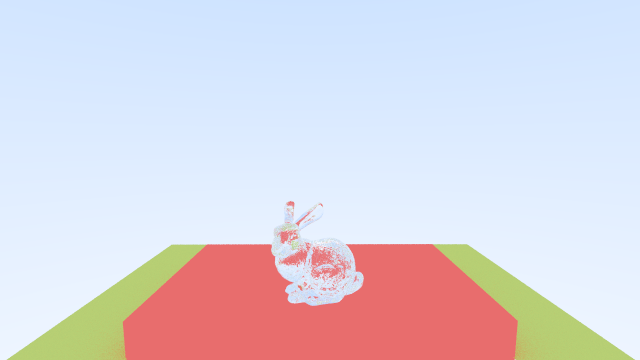
\includegraphics[scale=0.315]{media/bunny.png}
		\caption{light ON.}
		\label{light1}
	\end{subfigure}
	\begin{subfigure}{.48\textwidth}
		\centering
		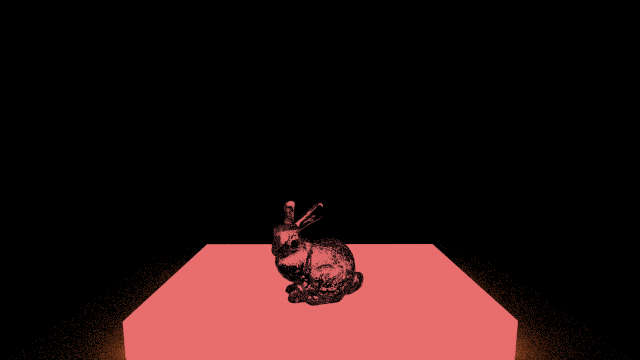
\includegraphics[scale=0.315]{media/bunny_noktem.png}
		\caption{light OFF.}
		\label{light2}
	\end{subfigure}
\end{figure}

We can observe how in the scene where we have the light "on", Figure \ref{light1}, we can see with total clarity all the objects of the scene, instead of the image with the light "off", Figure \ref{light2}, the only object that emits light is the red cube. You can see how the points closest of the green plane to the light source can be seen, while the rest of the scene remains dark.

\end{itemize}

\subsubsection{GPU parameters}

\begin{itemize}

\item \textbf{-nthreads} $n$

Optional parameter. It defines the number of threads we will use. The default value is 32.

\item \textbf{-nGPUs} $n$

Optional parameter. Sets the number of GPUs on which the application will run. The minimum value is 1 and the maximum is the maximum number of GPUs in our system. In the case of BOADA the range is $[1,4]$.


\end{itemize}

\section{Renderer}

The renderer is the entity in charge of launching the rays from the camera for each pixel and calculating their colour using the defined parameters.

The renderer varies a bit from the CPU and GPU versions because we can think as if the CPU has an infinite stack, but on the GPU we can't think this way. For this reason, the Algorithm \ref{color_alg_rec} instead of being recursive must be iterative. Moreover, not only this algorithm varies in both versions but also the path of the BVH. As we explained, a BVH is a tree-type data structure. The most natural way to go through a tree that we can think of is by a recursive algorithm, but as in the GPU we'll have many threads lacing up at the same time we can't make a thread occupy the whole stack, the overhead that is created affects negatively in the application's performance. That's why we'll implement an iterative algorithm to calculate the beam/BVH intersection to reduce the overhead as much as possible. We will be able to compare how using a recursive algorithm to go through the tree in the GPU drastically affects the performance.

\subsection{Sequential CPU}

\begin{algorithm}[caption={renderer sequential}, label={renderer_alg}]
input: int n, int m, int s, int d, Camera cam, Scene scene, bool light, bool sky, Skybox skybox
output: Image
begin
  Image $I(n,m)$
  foreach $(i,j) \in I$
    Colour $c = 0$
    foreach $s \in [1,s]$
      $u = \frac{i + random[0,1]}{nx}$
      $v = \frac{j + random[0,1]}{ny}$
      Ray $r \gets $ cam.getRay($u$, $v$);      
      $c += $ colour($r$, $d$, $0$, scene, light, sky, skybox)
    end
    $I(i,j) = \frac{c}{s}$
  end
  return $I$
end
\end{algorithm}

As we can see in the Algorithm \ref{renderer_alg} each pixel $(i,j)$ of the image $I$ is calculated from the surrounding pixels using the anti-aliasing technique explained in the introduction. For each sub-pixel $(u,v)$ we launch the primary ray from the camera and the \textbf{colour} function is responsible for integrating the rendering equation. For this, you need the scene, the primary ray $r$ and the bounce limit to cut the recursion. Then we also have the input parameters of the program \textit{light} and \textit{skybox} that tell us what type of background we use. We need them to know what colour we have to return when a ray \textit{gets lost} in the infinite.

The definition of the scene varies according to the type of representation we use. As we said, we have two versions one that represents the scene with a list of all the triangles of all the objects that compose the scene and another one in which we represent them with a BVH.

\begin{algorithm}[caption={colour recursive}, label={color_alg_rec}]
input: Ray r, int depth, int limit, Scene scene, bool light, bool sky, Skybox skybox
output: Colour
begin
  hit_record rec
  if collision(scene, $r$, rec)
    Ray scattered
    Colour attenuation
    Colour emitted = rec.Material.emission(rec.$u$, rec.$v$)
    if depth < limit and rec.Material.scatter($r$, rec, attenuation, scattered)
      return emitted + attenuation*color(scattered, depth+1, limit, scene, light, sky, skybox)
    else
      return emitted //light absorbed by light source.
  else
    if sky and collision(skybox, $r$, rec)
        return rec.Material.emission(rec.$u$, rec.$v$)
    else
      if light
        return blend(blue, white)
      else
        return black
end
\end{algorithm}

"hit\_record" is a data structure that allows us to store information regarding the point at which a lightning ray has collided. In it, we have, for example, the texture coordinates, the material of the impacted object, the new scattered ray, etc. This structure is initialized in the "collision" routine. This subroutine is the Möller-Trumbore algorithm, in the case of the version with BVH when we are in a leaf node, or the slab method in the case of an intermediate node in the version with BVH. The \textit{scatter} function represents the BRDF function.

\subsection{Parallel CPU}

For the parallel version of the renderer function, we have chosen a similar strategy to the construction of the BVH. Also, we will add the collapse directive to \textit{join} both loops, $i$ index loop and $j$ index loop, to distribute iterations to the threads. So, one thread has one $(i,j)$ iteration.

\begin{algorithm}[caption={renderer sequential}, label={renderer_cpu_par_alg}]
input: int n, int m, int s, int d, Camera cam, Scene scene, bool light, bool sky, Skybox skybox
output: Image
begin
  Image $I(n,m)$
  #pragma omp parallel for collapse(2) schedule(static,maxthreads)
  foreach $(i,j) \in I$
    Colour $c = 0$
    foreach $k \in [1,s]$
      $u = \frac{i + random[0,1]}{nx}$
      $v = \frac{j + random[0,1]}{ny}$
      Ray $r \gets $ cam.getRay($u$, $v$);      
      $c += $ colour($r$, $d$, $0$, scene, light, sky, skybox)
    end
    $I(i,j) = \frac{c}{s}$
  end
  return $I$
end
\end{algorithm}


\subsection{Parallel GPU}

As we discussed in the GPU version, it's best to take an iterative approach so that each thread runs in the same loop as many times as necessary without overspending memory. So the previously recursive algorithm (\ref{color_alg_rec}) is now iterative.

\begin{algorithm}[caption={colour recursive}, label={color_alg_it}]
input: Ray r, int limit, Scene scene, bool light, bool sky, Skybox skybox
output: Colour
begin
  Ray $current\_ray = r$ //first ray is the primary ray r
  $Vector_3 current\_attenuation = (1,1,1)$
  foreach $d \in [0,limit]$
    hit_record rec
    if collision(scene, $r$, rec)
      Ray scattered
      Colour attenuation
      Colour emitted = rec.Material.emission(rec.$u$, rec.$v$)
      
      if rec.Material.scatter($current_ray$, rec, attenuation, scattered)
        $current\_attenuation$ *= attenuation 
        $current\_attenuation$ += emitted
        $current\_ray = scattered$
      else
        return $current\_attenuation$ * emitted //light absorbed by light source
    else
      if sky and collision(skybox, $r$, rec)
        return rec.Material.emission(rec.$u$, rec.$v$)
      else
        if light
          return blend(blue, white)
        else
          return black      
  end
end
\end{algorithm}

For the configuration of the rendering kernel, we have followed the same strategy as for the construction of the BVH. In this case, if we have an $NX \times NY$ image we will store it in an array of an $NX \times NY$ size. This way the block distribution and indexing are simpler and more efficient. Therefore, we will have:

$$
BS = n
$$
$$
GS = \frac{(NX \times NY) + n - 1}{n}
$$

\begin{algorithm}[caption={kernel renderer GPU}, label={renderer_gpu_par_alg}]
input:Image I,  int n, int m, int s, int d, Camera cam, Scene scene, bool light, bool sky, Skybox skybox
output:
begin
  $idx = blockIdx.x * blockDim.x + threadIdx.$ 
  
  $i = idx \bmod n $
  $j = \frac{idx}{n} $
  
  Colour c = 0
  
  foreach $k \in [0,s] $
    $u = \frac{i + random[0,1]}{nx}$
    $v = \frac{j + random[0,1]}{ny}$
    Ray $r \gets $ cam.getRay($u$, $v$);      
    $c += $ colour($r$, $d$, $0$, scene, light, sky, skybox)
  end    

   $I_{idx} = c/s$  
  
end
\end{algorithm}

For the version where we can use \textit{n} GPUs, we have decided to distribute the image calculator by distributing it by blocks of rows. That is, each GPU will process a block of rows in an equitable ratio. If we think the image as an array instead of a matrix, we would be splitting it into \textit{n} equal pieces.

\begin{figure}[H]
	\centering
	\includegraphics[scale=0.50]{media/divideAndConquer.png}
	\caption{figure}{Image distribution for 4 GPUs.}
	\label{distribution}
\end{figure}

\chapter{Performance Experiments}

To test our application and determine which version is more efficient we will create three different scenes with certain characteristics. The first scene, Figure \ref{sc1}, is distinguished by having a low amount of polygons (72 triangles in the whole scene). The second scene, Figure [6], is characterized by a higher number of polygons than the first one (3040). And the last scene contains a much higher number of triangles than the two previous ones. A big difference between the first two and the third one is that the first ones are inside an enclosure, so most of the rays will exhaust the bounce limit established, except for those that reach a light source before. On the other hand, in the third one, we are outdoors, so it is much more probable that a ray escapes to the sky in fewer bounces than the limit established.

\section{Scene One}

As we can see in the image, this scene is composed of 4 cuboids. The one that makes up Cornell's box, the two central cubes and the light source. This is a scene with little geometry and hermetically sealed. There is only one light source, we don't have a sky where the rays can ''get lost'' so the probability of making all the imposed bounces is higher. One of the cubes, the tallest one, has a metal type material with a roughness index of 0, and the other cube has a diffuse material.

\begin{figure}[H]
	\centering
	\includegraphics[scale=0.50]{media/cornell_normal.png}
	\caption{figure}{Scene one. 200 samples pler pixel.}
	\label{sc1}
\end{figure}

If we look closely at the results table \ref{sc1}, we can see how the CUDA version is by far superior to the \texttt{OpenMP} version. While, it is true that with the \texttt{OpenMP} version we realize a great increase in performance, with \texttt{CUDA} we can improve it by up to 10 in some case. A significant highlight is the high potential of the new RTX cards. In the case of this scene, if we look at the column of 100 samples per pixel, we can see how the version that implements the ray/BVH intersection test in iterative matches (or improves) in time that making use of three BOADA GPUs.

If we look at the times of the \texttt{OpenMP} version, we see that the time difference in the different versions of the BVH does not affect it in the same way as it did in \texttt{CUDA}. 

The desktop version is superior in all versions with the experiments we have been able to perform. With respect to GPUs, it is the one with the best hardware. Regarding the CPU, it would have been interesting to try \texttt{OpenMP} in BOADA which has 32 threads against the 8 threads we can get in the CPU of the rest of the machines.

\subsection{Results}

\begin{table}[H]
    \centering
    \begin{adjustbox}{max width=\textwidth}
    \begin{tabular}{*{9}{|c}|}
         \hline
         \multicolumn{3}{|c|}{\multirow{2}{*}{Version}} & \multirow{2}{*}{Machine} & \multicolumn{5}{|c|}{Scene one} \\
         \multicolumn{3}{|c|}{} &  & \multicolumn{5}{|c|}{Time (\textit{seconds})}  \\ \hline
         & & & & 1 sample(s) & 10 sample(s) & 50 sample(s) & 100 sample(s) & 200 sample(s) \\ \hline
         \multirow{12}*{CPU} & \multirow{6}*{Seq.}  & 
         	\multirow{2}*{List} & 
         		Lenovo 	& 15,50 & 154,14 & 774,44 & 1542,36 & 3095,65 \\ \cline{4-9}
         	& & &
         		Desktop & 14,12 & 139,79 & 742,83 & 1445,64 & 2809,16 \\ \cline{3-9}
		 & &        	
         	\multirow{2}*{BVH It.} &
         		Lenovo 	& 30,85 & 300,05 & 1493,99 & 3045,05 & 6081,05 \\ \cline{4-9}
         	& & &
         		Desktop & 27,51 & 273,01 & 1369,04 & 2729,36 & 5462,02 \\ \cline{3-9}
         & &        	
         	\multirow{2}*{BVH Rec.} &
         		Lenovo 	& 28,22 & 282,373 & 1407,27 & 2815,23 & 5632,42 \\ \cline{4-9}
         	& & &
         		Desktop & 26,06 & 258,99 & 1285,07 & 2568,13 & 5156,55  \\ \cline{2-9}
         		
         & \multirow{6}*{\texttt{OpenMP}}  &
         	\multirow{2}*{List} & 
         		Lenovo 	& 9,54 & 94,16 & 480,20 & 982,87 & 1929,72 \\ \cline{4-9}
         	& & &
         		Desktop & 8,79 & 88,81 & 460,89 & 877,24 & 1859,07 \\ \cline{3-9}
		 & &        	
         	\multirow{2}*{BVH It.} &
         		Lenovo 	&  10,08 & 102,17 & 525,59 & 1194,84 & 2159,8\\ \cline{4-9}
         	& & &
         		Desktop & 9,01 & 90,48 & 451,49 & 916,96 & 1801,08\\ \cline{3-9}
         & &        	
         	\multirow{2}*{BVH Rec.} &
         		Lenovo 			& 11,40 & 122,50 	& 601,731 	& 1169,89 	& 2033,67  \\ \cline{4-9}
         	& & &
         		Desktop 		& 9,24 	& 88,62 	& 449,78 	& 896,47 	& 1762,38  \\ \cline{1-9}
         		
         \multirow{18}*{GPU} & \multirow{18}*{\texttt{CUDA}} &
         	\multirow{6}*{List} & 
         		Lenovo 			& 2,58 	& 25,76 & 128,43 	& 257,42	& 513,87	\\ \cline{4-9}
         	& & &
         		Desktop 		& 0,93 	& 9,38 	& 46,57 	& 91,85 	& 187,2    	\\ \cline{4-9}
         	& & &
         		BOADA - 1 GPU(s) 	& 3,13  & 27,53 & 135,83  	& 271,39 	& -   		\\ \cline{4-9}
         	& & &
         		BOADA - 2 GPU(s) 	& 2,07 	& 14,88 & 71,67 	& 142,867 	& 285,18   	\\ \cline{4-9}
         	& & &
         		BOADA - 3 GPU(s) 	& 1,87 	& 10,58 & 49,32 	& 97,80 	& 194,22   	\\ \cline{4-9}
         	& & &
         		BOADA - 4 GPU(s) 	& 1,83 	& 8,45 	& 37,77 	& 74,38 	& 147,36 	\\ \cline{3-9} % 220,256 & 293,77
		 & &        	
         	\multirow{6}*{BVH It.} &
         		Lenovo 	& 5,68 & 56,58 & 285,36 &  1138,34  & 1703,40  \\ \cline{4-9}
         	& & &
         		Desktop & 1,495 & 15,11 & 75,14 & 149,00 & 300,13 \\ \cline{4-9}
         	& & &
         		BOADA - 1 GPU(s) & 4,46 & 45,66 & 226,37 &  452,18 & -   \\ \cline{4-9}
         	& & &
         		BOADA - 2 GPU(s) & 3,05 & 24,26 & 118,67 &  236,20 &  - \\ \cline{4-9}
         	& & &
         		BOADA - 3 GPU(s) & 2,53 & 16,66 & 79,75 & 158,22 & 316,99 \\ \cline{4-9}
         	& & &
         		BOADA - 4 GPU(s) & 2,40 & 13,17  & 61,34 & 120,84  & 240,43 \\ \cline{3-9}
         & &        	
         	\multirow{6}*{BVH Rec.} &
         		Lenovo 	& 6,09 & 60,79 & 304,07 & 608,53 & 1216,93  \\ \cline{4-9}
         	& & &
         		Desktop &  9,09 & 108,15 & 557,74 & 1092,76 & -   \\ \cline{4-9}
         	& & &
         		BOADA - 1 GPU(s) & 21,64 & 212,176 & - &  - & -   \\ \cline{4-9}
         	& & &
         		BOADA - 2 GPU(s) & 11,83 & 111,84 & 555,42 & - & - \\ \cline{4-9}
         	& & &
         		BOADA - 3 GPU(s) & 8,51 & 75,54 & 375,68 & - & - \\ \cline{4-9}
         	& & &
         		BOADA - 4 GPU(s) & 6,99 & 57,98 & 284,42 & - & - \\ \cline{1-9}
         	
    \end{tabular}
    \end{adjustbox}
    \caption{Scene one time table}
    \label{tab:scene1}
\end{table}

\section{Scene Two}

The next scene follows the same concept as the previous one, but now instead of having two cubes we have two 3D models of a reindeer. One of them is defined with a diffuse material, and the other one is made of glass. Also, the floor of the room is mirror-like. Now the complexity of the scene lies in the number of polygons.

If we look carefully at the table of results \ref{sc2}, we can see how now the BVH has the effect we were looking for. Boost the performance of the application. If we compare the iterative version of the BVH against the representation version using a list, we see that the first one is up to ten times faster than the second option. For a scene with more than a thousand triangles, not using any parallelization tool is a waste of time. We can wait for hours to finish rendering the output image.

\subsection{Results}

\begin{table}[H]
    \centering
    \begin{adjustbox}{max width=\textwidth}
    \begin{tabular}{*{9}{|c}|}
         \hline
         \multicolumn{3}{|c|}{\multirow{2}{*}{Version}} & \multirow{2}{*}{Machine} & \multicolumn{5}{|c|}{Scene one} \\
         \multicolumn{3}{|c|}{} &  & \multicolumn{5}{|c|}{Time (\textit{seconds})}  \\ \hline
         & & & & 1 sample(s) & 10 sample(s) & 50 sample(s) & 100 sample(s) & 200 sample(s) \\ \hline
         \multirow{12}*{CPU} & \multirow{6}*{Seq.}  & 
         	\multirow{2}*{List} & 
         		Lenovo 			& & & & &  \\ \cline{4-9}
         	& & &
         		Desktop 		& & & & &  \\ \cline{3-9}
		 & &        	
         	\multirow{2}*{BVH It.} &
         		Lenovo 			& & & & & \\ \cline{4-9}
         	& & &
         		Desktop		 	& & & & &  \\ \cline{3-9}
         & &        	
         	\multirow{2}*{BVH Rec.} &
         		Lenovo 			& & & & &   \\ \cline{4-9}
         	& & &
         		Desktop 		& & & & &  \\ \cline{2-9}
         		
         & \multirow{6}*{\texttt{OpenMP}}  &
         	\multirow{2}*{List} & 
         		Lenovo 			& & & & & \\ \cline{4-9}
         	& & &
         		Desktop 		& & & & & \\ \cline{3-9}
		 & &        	
         	\multirow{2}*{BVH It.} &
         		Lenovo 			& & & & &	\\ \cline{4-9}
         	& & &
         		Desktop 		& & & & &	\\ \cline{3-9}
         & &        	
         	\multirow{2}*{BVH Rec.} &
         		Lenovo 			& & & & &  \\ \cline{4-9}
         	& & &
         		Desktop 		& & & & & 	\\ \cline{1-9}
         		
         \multirow{18}*{GPU} & \multirow{18}*{\texttt{CUDA}} &
         	\multirow{6}*{List} & 
         		Lenovo 			& 107,52 & 1075,6 & & & \\ \cline{4-9}
         	& & &
         		Desktop 		& 28,19 & 297,74 & 1473,80 & 2928,41 &   	\\ \cline{4-9}
         	& & &
         		BOADA - 1 GPU(s) 	& 89,72 & - & - & - & -		\\ \cline{4-9}
         	& & &
         		BOADA - 2 GPU(s) 	& 47,12 & 466,79 & - & - & - 	\\ \cline{4-9}
         	& & &
         		BOADA - 3 GPU(s) 	& 32,19 & 313,57 & - & - & -  	\\ \cline{4-9}
         	& & &
         		BOADA - 4 GPU(s) 	& 24,86 & 236,67 & - & - & -  \\ \cline{3-9} % 220,256 & 293,77
		 & &        	
         	\multirow{6}*{BVH It.} &
         		Lenovo 			& 21,05 & 206,84 & 1031,70 & 2076,09 &  \\ \cline{4-9}
         	& & &
         		Desktop 		& 2,88 & 28,578 & 145,64 & 281,75 & 561,86	\\ \cline{4-9}
         	& & &
         		BOADA - 1 GPU(s) 	& 13,82 & 131,13 & 650,972 & - & - 	\\ \cline{4-9}
         	& & &
         		BOADA - 2 GPU(s) 	& 7,49 & 69,67 & 344,18 & - & - 	\\ \cline{4-9}
         	& & &
         		BOADA - 3 GPU(s) 	& 5,56 & 46,65 & 228,36 & 456,21 & - 	\\ \cline{4-9}
         	& & &
         		BOADA - 4 GPU(s) 	& 4,83 & 36,34 & 178,22 & 353,11 & - 	\\ \cline{3-9}
         & &        	
         	\multirow{6}*{BVH Rec.} &
         		Lenovo 			& 42,59 & 425,59 & 2123,99 & 4253,62 & 8512,77 	\\ \cline{4-9}
         	& & &
         		Desktop 		& 20,70 & 236,11 & 1252,08 & 2736,14 & -   \\ \cline{4-9}
         	& & &
         		BOADA - 1 GPU(s) 	& 40,82 & 402,58 & - & - & -   \\ \cline{4-9}
         	& & &
         		BOADA - 2 GPU(s) 	& 21,92 & 214,38 & - & - & - \\ \cline{4-9}
         	& & &
         		BOADA - 3 GPU(s) 	& 15,09 & 142,44 & - & - & -	\\ \cline{4-9}
         	& & &
         		BOADA - 4 GPU(s) 	& 10,23 & 120,35 & - & - & - 	\\ \cline{1-9}
         	
    \end{tabular}
    \end{adjustbox}
    \caption{Scene two time table}
    \label{sc2}
\end{table}

\section{Scene three}

\subsection{Results}

\begin{table}[H]
    \centering
    \begin{adjustbox}{max width=\textwidth}
    \begin{tabular}{*{9}{|c}|}
         \hline
         \multicolumn{3}{|c|}{\multirow{2}{*}{Version}} & \multirow{2}{*}{Machine} & \multicolumn{5}{|c|}{Scene one} \\
         \multicolumn{3}{|c|}{} &  & \multicolumn{5}{|c|}{Time (\textit{seconds})}  \\ \hline
         & & & & 1 sample(s) & 10 sample(s) & 50 sample(s) & 100 sample(s) & 200 sample(s) \\ \hline
         \multirow{12}*{CPU} & \multirow{6}*{Seq.}  & 
         	\multirow{2}*{List} & 
         		Lenovo 			& & & - & - & -  \\ \cline{4-9}
         	& & &
         		Desktop 		& & & - & - & -  \\ \cline{3-9}
		 & &        	
         	\multirow{2}*{BVH It.} &
         		Lenovo 			& & & - & - & - \\ \cline{4-9}
         	& & &
         		Desktop		 	& & & - & - & -  \\ \cline{3-9}
         & &        	
         	\multirow{2}*{BVH Rec.} &
         		Lenovo 			& & & - & - & -   \\ \cline{4-9}
         	& & &
         		Desktop 		& & & - & - & - \\ \cline{2-9}
         		
         & \multirow{6}*{\texttt{OpenMP}}  &
         	\multirow{2}*{List} & 
         		Lenovo 			& & & - & - & - \\ \cline{4-9}
         	& & &
         		Desktop 		& & & - & - & - \\ \cline{3-9}
		 & &        	
         	\multirow{2}*{BVH It.} &
         		Lenovo 			& & & & - & -	\\ \cline{4-9}
         	& & &
         		Desktop 		& & & & - & -	\\ \cline{3-9}
         & &        	
         	\multirow{2}*{BVH Rec.} &
         		Lenovo 			& & & & - & -  \\ \cline{4-9}
         	& & &
         		Desktop 		& & & & - & - 	\\ \cline{1-9}
         		
         \multirow{18}*{GPU} & \multirow{18}*{\texttt{CUDA}} &
         	\multirow{6}*{List} & 
         		Lenovo 			& 144,05 &  &  & - & - \\ \cline{4-9}
         	& & &
         		Desktop 		& 121,31 & 1320,21 & 6472,71 & - & -  	\\ \cline{4-9}
         	& & &
         		BOADA - 1 GPU(s) 	& 402,82 & - & - & - & -	\\ \cline{4-9}
         	& & &
         		BOADA - 2 GPU(s) 	& 221,20 & - & - & - & - 	\\ \cline{4-9}
         	& & &
         		BOADA - 3 GPU(s) 	& 185,33 & - & - & - & - 	\\ \cline{4-9}
         	& & &
         		BOADA - 4 GPU(s) 	& 144,05 & - & - & - & -  \\ \cline{3-9} % 220,256 & 293,77
		 & &        	
         	\multirow{6}*{BVH It.} &
         		Lenovo 				& 1,55 & 15,43 & 76,68 & 153,65 & 307,55 \\ \cline{4-9}
         	& & &
         		Desktop 			& 0,27 & 2,38 & 11,93 & 23,6 & 45,94 \\ \cline{4-9}
         	& & &
         		BOADA - 1 GPU(s) 	& 2,25 & 17,46 & 85,99 & 169,99 & 339,61 	\\ \cline{4-9}
         	& & &
         		BOADA - 2 GPU(s) 	& 1,88 & 9,46 & 45,72 & 90,15 & 178,83\\ \cline{4-9}
         	& & &
         		BOADA - 3 GPU(s) 	& 2,04 & 9,42 & 41,60 & 82,52 & 168,632 	\\ \cline{4-9}
         	& & &
         		BOADA - 4 GPU(s) 	& 2,29 & 7,98 & 33,77 & 65,64 & 128,26	\\ \cline{3-9}
         & &        	
         	\multirow{6}*{BVH Rec.} &
         		Lenovo 				& 4,42 & 39,62 & 198,03 & 398,34 & 793,71	\\ \cline{4-9}
         	& & &
         		Desktop 			& 2,51 & 26,99 & 137,24 & 284,24 &  567,90 \\ \cline{4-9}
         	& & &
         		BOADA - 1 GPU(s) 	& 6,99 & 63,56 & 316,55 & - & -  \\ \cline{4-9}
         	& & &
         		BOADA - 2 GPU(s) 	& 4,29 & 34,10 & 164,44 & 330,92 & - \\ \cline{4-9}
         	& & &
         		BOADA - 3 GPU(s) 	& 4,347 & 32,79 & 158,46 & 317,07 & -	\\ \cline{4-9}
         	& & &
         		BOADA - 4 GPU(s) 	& 3,93 & 25,69 & 123,68 & 243,43 & - 	\\ \cline{1-9}
         	
    \end{tabular}
    \end{adjustbox}
    \caption{Scene three time table}
    \label{sc3}
\end{table}

\section{Conclusion and Future Work}

First of all, I would like to comment on the limitation that the environment of BOADA has given us for the phase of experimentation and testing of the applications. At the beginning, the intention was to test the four GPUs that BOADA offers us, but due to the fact that it is a teaching and research cluster, we do not have its resources infinitely as it is the case of our personal computers. The processes that are launched to the execution queue have a limited life limit so the more samples per pixel we add to our render, the more expensive it is and in the end, the system rejects it. In the case of Scene 2, you can see how this limitation has impacted the results, especially in the version without the optimization of the BVH.

Undoubtedly we see how for relatively small scenes (<500~1000 triangles) the BVH introduces a huge expense for all versions. So for these cases it would be better not to use this data structure. Instead, for scenes with a large geometry, the use of these data structures is crucial for the performance of the application.

Another observation to emphasize is that indeed the recursion affects negatively to the performance of the program as we have commented previously. The most affected GPU has been undoubtedly the Tesla K40c from BOADA, where a single GPU for a sample per pixel has taken 21 seconds, more than double than the RTX 2080 Super and triple than the GTX 1050 M. The RTX 2080 proved to be superior among all GPUs, matching or even improving the time of the version using three Tesla K40c.

As expected, the slowest version is the sequential one. There's no reason to not take the advantage of the parallel capability that our computers offer us today.  And without a doubt, GPUs are the best option of all, offering us between 7 and 10 times more performance than using only the CPU.

In conclusion, GPUs are the most suitable tool for applications where we require great computing power. Today, with the new RTXs we can perform real-time Ray Tracing thanks to a pipeline-graphic hybrid between Ray Tracing and traditional rasterization.

\section{Future Work}

I still have a lot of work to do in this wonderful branch of computer graphics such as offline rendering and realistic rendering. My intention is to continue progressing and expanding my knowledge in order to improve this application by adding new lighting models such as \citep[pp.~25--32]{Ashikhmin2000} or \citep[pp.~239--246]{Oren1994}, particle system, subsurface scattering, and a long list of other features. 

Perhaps in the future we will be able to render photo-realistic images in real time without the need for filtering and hybrid systems.


\newpage

\printbibliography

\begin{appendices}
\chapter{Gantt Diagram}

\uselandscape

\begin{figure}[H]
	\centering
	\includegraphics[scale=0.30]{media/final_gantt_esp.png}
	\captionof{figure}{Complete Gantt Chart.}
	\label{gantt_esp}
\end{figure}

\begin{figure}[H]
	\centering
  	\includegraphics[scale=0.25]{media/gantt_gep.png}
  	\captionof{figure}{GEP Stage.}
  	\label{gantt_1}
\end{figure}

\begin{figure}[H]
	\centering
  	\includegraphics[scale=0.25]{media/gantt_dev_esp.png}
  	\captionof{figure}{Development Stage.}
  	\label{gantt_2}
\end{figure}

\begin{figure}[H]
	\centering
	\includegraphics[scale=0.30]{media/final_gantt_eng.png}
	\captionof{figure}{Complete Gantt Chart.}
	\label{gantt_eng}
\end{figure}

\begin{figure}[H]
	\centering
  	\includegraphics[scale=0.25]{media/gantt_dev_eng_new.png}
  	\captionof{figure}{Development Stage new tasks.}
  	\label{gantt_3}
\end{figure}

\begin{figure}[H]
	\centering
  	\includegraphics[scale=0.25]{media/gantt_final_eng.png}
  	\captionof{figure}{Final Stage.}
  	\label{gantt_4}
\end{figure}

\useportrait

\end{appendices}

\listoffigures

\listoftables

\end{document}
